\documentclass[review,onefignum,onetabnum]{siamart190516}
%Packages
\usepackage[utf8]{inputenc}
\usepackage{geometry, graphicx,wrapfig}
\usepackage{enumerate}
\usepackage{amsmath,amssymb,amsfonts,bm}
\usepackage{xcolor} %just for visible comments.
\usepackage[linesnumbered,ruled,vlined,algo2e]{algorithm2e}
\usepackage[toc,page]{appendix}
\usepackage{makecell}
\usepackage{cleveref}

% New theorems and commands
\newtheorem{assump}[theorem]{MP Setting}
\newcommand\mycommfont[1]{\ttfamily\textcolor{orange}{#1}}
\newcommand{\R}{\mathbb{R}}
\newcommand{\F}{\mathbb{F}}
\newcommand{\dd}{\delta}
\newcommand{\tth}{\theta}
\newcommand{\bb}[1]{\mathbf{#1}}
\newcommand{\fl}{\mathrm{fl}}
\newcommand{\cO}{\mathcal{O}}

\newcommand\blfootnote[1]{%
	\begingroup
	\renewcommand\thefootnote{}\footnote{#1}%
	\addtocounter{footnote}{-1}%
	\endgroup
}

\setlength{\abovedisplayshortskip}{0pt}
\setlength{\belowdisplayshortskip}{0pt}

\crefname{algocf}{alg.}{algs.}
\Crefname{algocf}{Algorithm}{Algorithms}

% Document
\title{Rounding Error Analysis of Mixed Precision Block Householder QR Algorithms}
\author{L. Minah Yang, Alyson Fox, and Geoffrey Sanders}
\date{\today}
\begin{document}

\maketitle
\begin{abstract}
	Although mixed precision arithmetic has recently garnered interest for training dense neural networks, many other applications could benefit from the  speed-ups and lower storage cost if applied appropriately. 
	The growing interest in employing mixed precision computations motivates the need for rounding error analysis that properly handles behavior from mixed precision arithmetic.
	We develop mixed precision variants of existing Householder QR algorithms and show error analyses supported by numerical experiments.	\blfootnote{This work was performed under the auspices of the U.S. Department of Energy by Lawrence Livermore National Laboratory under Contract DE-AC52-07NA27344 and was supported by the LLNL-LDRD Program under Project No. 17-SI-004, LLNL-JRNL-795525-DRAFT.}
\end{abstract}
\section{Introduction}\label{sec:intro}
%%The accuracy of a numerical algorithm depends on several factors, including numerical stability and well-conditionedness of the problem, both of which may be sensitive to rounding errors, the difference between exact and finite-precision arithmetic. 
%Low precision floats use fewer bits than high precision floats to represent the real numbers and naturally incur larger rounding errors. 
%Therefore, error attributed to round-off may have a larger influence over the total error when using low precision, and some standard algorithms may yield insufficient accuracy when using low precision storage and arithmetic.
%%TODO: MINAH comment reviewer 
%%that are in wide use may no longer be numerically stable when using half precision floating arithmetic and storage. 
%However, many applications exist that would benefit from the use of lower precision arithmetic and storage that are less sensitive to floating-point round off error, such as clustering or ranking graph algorithms \cite{vonLuxburg2007} or training dense neural networks \cite{micikevicius2018mixed}, to name a few.\par
%
%Many computing applications today require solutions quickly and often under low size, weight, and power constraints (low SWaP), e.g., sensor formation, etc. 
%%TODO: Reviewer #2 asks what does weight mean here.
%Computing in low-precision arithmetic offers the ability to solve many problems with improvement in all four parameters.
%Utilizing mixed precision, one can achieve similar quality of computation as high-precision and still achieve 
%speed, size, weight, and power constraint improvements. 
%There have been several recent demonstrations of computing using half-precision arithmetic (16 bits) achieving around half an order to an 
%order of magnitude improvement of these categories in comparison to double precision (64 bits).
%Trivially, the size and weight of memory required for a specific problem is 4$\times$.
%Additionally, there exist demonstrations that the power consumption improvement is similar
%\cite{fagan2016powerwall}.
%Modern accelerators (e.g., GPUs, Knights Landing, or Xeon Phi) are able to achieve this factor or better speedup improvements.
%Several examples include:
%(i)   2-4$\times$ speedup in solving dense large linear equations \cite{haidar2018iterative,haidar2019tensorcore},
%(ii)  12$\times$ speedup in training dense neural networks,
%and
%(iii) 1.2-10$\times$ speedup in small batched dense matrix multiplication \cite{abdelfattah2019batched} (up to 26$\times$ for batches of tiny matrices).
%Training deep artificial neural networks by employing lower precision arithmetic to various tasks such as multiplication \cite{Courbariaux2014Mult} and storage \cite{Courbariaux2014Storage} can easily be implemented on GPUs and are already a common practice in data science applications.\par
%
%The low precision computing environments that we consider are \emph{mixed precision} settings, which are designed to imitate those of new GPUs that employ multiple precision types for certain tasks. 
%For example, Tesla V100's TensorCores perform matrix products of half precision input data with exact products and single precision (32 bits) summation accumulate \cite{nvdia}.
%The existing rounding error analyses are built within what we call a \emph{uniform precision} setting, which is the assumption that all arithmetic operations and storage are performed via the same precision.
%In this work, we develop a framework for deterministic mixed precision rounding error analysis, and explore half-precision Householder QR factorization (HQR) algorithms for data and graph analysis applications. 
%QR factorization is known to provide a backward stable solution to the linear least squares problem and thus, is ideal for mixed precision. 
%%TODO: Remove it and just explain in response to reviewers. didn't serve purpose of paper mixed precision is an active area of research
%%TODO: algorithms with better stability should be looked at first in mixed precision. 
%
%However, additional analysis is needed as the additional round-off error will effect orthogonality, and thus the accuracy of the solution. 
%Here, we focus on analyzing specific algorithms in a specific set of types (IEEE754 half (fp16), single (fp32), and double(fp64)), but the framework we develop 
%could be used on different algorithms or different floating point types (such as bfloat16 in \cite{tagliavini2018floating}).\par
%
%This work discusses several aspects of using mixed precision arithmetic: (i) error analysis that can more accurately describe mixed precision arithmetic than existing analyses, (ii) algorithmic design that is more resistant against lower numerical stability associated with lower precision types, and (iii) an example where mixed precision implementation performs as sufficiently as double-precision implementations. 
%Our key findings are that the new mixed precision error analysis produces tighter error bounds, that some block QR algorithms by Demmel et al. \cite{Demmel2012} are able to operate in low precision more robustly than non-block techniques, and that some small-scale benchmark graph clustering problems can be successfully solved with mixed precision arithmetic.
%%TODO: MINAH rewrite outline of paper paragraph, and remove graph references in above paragraph.
%%In Section~\ref{sec:FPREA}, we will give an overview of the modern developments in hardware that motivates rounding error analysis that supports multiple precision types, and we will present a set of error analysis tools. 
%%The HQR factorization algorithm and a mixed precision rounding error analysis of its implementation is discussed in Section~\ref{sec:HQRf}.
%%In Section~\ref{sec:TSQR}, we present the TSQR algorithm as well as numerical experiments that show that TSQR can be useful in low precision environments. Section~\ref{sec:Apps} explores the use of low and mixed precision QR algorithms as subroutines for an application: spectral clustering.
The accuracy of a numerical algorithm depends on several factors, including numerical stability and well-conditionedness of the problem, both of which may be sensitive to rounding errors, the difference between exact and finite precision arithmetic. 
Low precision floats use fewer bits than high precision floats to represent the real numbers and naturally incur larger rounding errors. 
Therefore, error attributed to round-off may have a larger influence over the total error and some standard algorithms may yield insufficient accuracy when using low precision storage and arithmetic.
However, many applications exist that would benefit from the use of low precision arithmetic and storage that are less sensitive to floating-point round-off error, such as clustering or ranking graph algorithms \cite{vonLuxburg2007} or training dense neural networks \cite{micikevicius2018mixed}.\par

Many computing applications today require solutions quickly and often under low size, weight, and power constraints, such as in sensor formation, where low precision computation offers the ability to solve many problems with improvement in all four parameters.
Utilizing mixed precision, one can achieve similar quality of computation as high precision and still achieve 
speed, size, weight, and power constraint improvements. 
There have been several recent demonstrations of computing using IEEE half precision (fp16) achieving around half an order to an order of magnitude improvement of these categories in comparison to single and double precision (fp32, fp64).
Trivially, the size and weight of memory required for a specific problem is 4$\times$.
Additionally, there exist demonstrations that the power consumption improvement is similar
\cite{fagan2016powerwall}.
Modern accelerators (e.g., GPUs, Knights Landing, or Xeon Phi) are able to achieve this factor or better speedup improvements.
Several examples include:
(i)   2-4$\times$ speedup in solving dense large linear equations \cite{haidar2018iterative,haidar2019tensorcore},
(ii)  12$\times$ speedup in training dense neural networks,
and
(iii) 1.2-10$\times$ speedup in small batched dense matrix multiplication \cite{abdelfattah2019batched} (up to 26$\times$ for batches of tiny matrices).
Training deep artificial neural networks by employing lower precision arithmetic to various tasks such as multiplication \cite{Courbariaux2014Mult} and storage \cite{Courbariaux2014Storage} can easily be implemented on GPUs and are a common practice in some data science applications.\par

The low precision computing environments that we consider are \emph{mixed precision} settings, which are designed to imitate those of new GPUs that employ multiple precision types for certain tasks. 
For example, Tesla V100's TensorCores perform block Fused Multiply Add operations (bFMAs), where matrix products of fp16 input data can be computed up to $16\times$ faster than that of fp64.
The existing rounding error analyses of linear algebra routines are built within what we call a \emph{uniform precision} setting, which is the assumption that all arithmetic operations and storage are performed via the same precision.
In this work, we develop mixed precision variants of existing Householder (HH) QR factorization algorithms and perform mixed precision error analysis.
This work focuses on analyzing a few algorithms that use fp16/fp32 as the low/high precision types, but the error analysis can be easily modified for different floating point types (such as bfloat16 in \cite{tagliavini2018floating}).
The standard HH QR algorithm and its block variants that partition the columns (level-3 BLAS variant, see \cite{golub2013matrix,Higham2002}) and those that partition the rows (communication-avoiding algorithms of \cite{Demmel2012}) are presented in \cref{sec:algo}, then modified to support bFMAs and an ad hoc mixed precision setting that mimics NVIDIA TensorCores in \cref{sec:mpanalysis}.
Our key findings are that mixed precision error analyses produce tighter error bounds as supported by experiments in \cref{sec:NE}, algorithms that utilize level-3 BLAS operations can easily be modified to incorporate TensorCore bFMAs, and a row partition block algorithm operates  more robustly in mixed precision than non-block techniques in certain regimes.
\section{Background: Build up to rounding error analysis for inner products}\label{sec:background}
In this section, we introduce the basic motivations and tools for mixed precision rounding error analysis needed for the {\it QR factorization}.
A matrix $\bb{A} \in \R^{m \times n}$ for $m\geq n$ can be written as
\[\bb{A} = \bb{QR}=\begin{bmatrix}\bb{Q}_{1} & \bb{Q}_2\end{bmatrix} \begin{bmatrix}\bb{R}_{1} \\ \bb{0}_{m-n \times n}\end{bmatrix} = \bb{Q}_{1}\bb{R}_{1},\vspace{-0.3cm}
\]
where an orthogonal $\bb{Q}\in\R^{m\times m}$ and an upper trapezoidal $\bb{R}$ form a \emph{full} QR factorization, and $\bb{Q}_{1}\in\R^{m\times n},\bb{R}_{1}\in\R^{n\times n}$ form a \emph{thin} QR factorization.
If $\bb{A}$ is full rank then the columns of $\bb{Q}_{1}$ are orthonormal
and $\bb{R}_1$ is upper triangular.
In many applications, computing the \emph{thin} decomposition requires less computation and is sufficient in performance. 
While important definitions are stated explicitly in the text, Table~\ref{table:notation} serves to establish basic notation.
%\begin{table}[H]
	\centering
	%\begin{tabular}{|m{3cm}|m{9cm}|c|}
	\begin{tabular}{|m{1.7cm}|m{10.3cm}|c|}
		\hline
		%DONE: change table have the following 3 columns, add sections
		Symbol(s) & Definition(s) & Section(s) \\ \hline
		${\bb x}$, ${\bb A}$  & Vector, matrix  & \ref{sec:background} \\
		%	${\bb A}$ & Matrix & \ref{sec:intro}\\
		%$m$, $n$ & Number of rows, columns of matrix, or length of vector&  \ref{sec:intro}\\
		%$i$, $j$ & Row, column index of matrix or vector & \ref{sec:HQRfA} \\
		%$\|{\bf x}\|_2$, $\|\bb{A}\|_2$ & Vector operator 2-norm & \ref{sec:HQRf}\\
		%$|c|$, $|\bb{x}|$ ,$|\bb{A}|$ & Absolute value of constant, all elements of vector, matrix & \ref{sec:HQRf} \\
		%$\bb{x}_i$, $\hat{e}_i$  & $i^{th}$ element of vector $\bb{x}$, cardinal vector &  \ref{sec:HQRfA}, \ref{sec:HQRf}\\
		%$\bb{A}[a:b, c:d]$ &Rows $a$ to $b$ and columns $c$ to $d$ of matrix $\bb{A}$ & \ref{sec:HQRfA}\\
		%$\bb{A}[a:b,:]$, $\bb{A}[:,c:d]$ & Rows $a$ to $b$, columns $c$ to $d$ of matrix $\bb{A}$& \ref{sec:HQRfA}\\
		\hline
		$\bb{Q}$  & Orthogonal factor $\bb{A}\in\R^{m\times n}$: $m$-by-$m$ (full) or $m$-by-$n$ (thin)  & \ref{sec:background}\\
		$\bb{R}$ & Upper triangular or trapezoidal factor of $\bb{A}\in\R^{m\times n}$:  $m$-by-$n$ (full) or $n$-by-$n$ (thin)  &  \ref{sec:background}\\ 
		%$\bb{A}^{(k)}$ & Matrix $\bb{A}$ after $k$ Householder transformations. &\ref{sec:HQRfA}\\
		\hline
		$\fl(\bb{x})$, $\hat{\bb{x}}$ & Quantity $\bb{x}$ calculated from floating point operations & \ref{sec:backgroundRE} \\
		$b$, $t$, $\mu$, $\eta$  & Base/precision/mantissa/exponent bits & \ref{sec:backgroundRE} \\
		%\tt{Inf} & Values outside the range of representable numbers & \ref{sssec:NormalizeHV} \\ %https://www.doc.ic.ac.uk/~eedwards/compsys/float/nan.html
		$k$ & Number of successive FLOPs &  \ref{sec:backgroundRE}\\
		$u^q$ & Unit round-off for precision $t_q$ and base $b_q$: $\frac{1}{2}b_q^{1-t_q}$ & \ref{sec:backgroundRE} \\ 
		$\dd^{q}$ &Quantity bounded by: $|\dd^{q}| < u^q$ &  \ref{sec:backgroundRE} \\
		$\gamma^{q}_{k}$,  $\tth^{q}_{k}$& $\frac{ku^q}{1-ku^q}$, Quantity bounded by: $|\tth^{q}_{k}|\leq\gamma^q_{k}$ &  \ref{sec:backgroundRE} \\
		%$\tth_{q}^{(k)}$ & Quantity bounded by: $|\tth_{q}^{(k)}|\leq\gamma_q^{(k)}$ &  \ref{sec:FPREA} \\ 
		\hline
			%$\bb{0}_{m\times n}$, $\bb{I}_{n}$ & $m$-by-$n$ zero matrix, $n$-by-$n$ identity  matrix &  \ref{sec:intro}\\
		%$\bb{I}_{n} & $n$-by-$n$ identity  matrix  & \ref{sec:HQRfA} \\
		%$\bb{I}_{m\times n}$ & $[\bb{I}_{n} \quad \bb{0}_{n \times (m-n)}]^{\top}$ & \ref{sec:TSQR}\\ \hline
		%$\bb{P}_{\bb{v}}$, $\bb{P}_i$ & Householder transformation define by $\bb{v}$, $i^{th}$ Householder transformation in HQR& \ref{sec:HQRfA}\\
		%$\bb{P}_i$ & $i^{th}$ Householder transformation in the HQR algorithm & \ref{sec:HQRfA} \\ 
		\hline		
		%$u^h, u^l, u_w$ & Unit round-off for sum, product, and storage (write) & \ref{ssec:IP}\\ 
		%		$\gamma_{p,q}^{(k_l,k_q)}$ & $(1+\gamma_p^{(k_l)})(1+\gamma_q^{(k_q)})-1$ & \ref{ssec:IP}\\
		%		$\tth_{p,q}^{(k_l,k_q)}$ & Quantity bounded by: $|\tth_{p,q}^{(k_l,k_q)}|<\gamma_{p,q}^{(k_l,k_q)}$ & \ref{ssec:IP}\\
		\hline
	\end{tabular}
	\caption{Basic definitions}
	\label{table:notation}
\end{table}
\begin{table}[H]
	\centering
	\begin{tabular}{|m{2.cm}|m{10.6cm}|c|}
		\hline
		Symbol & Definition & Section \\ \hline
		${\bb x}$, ${\bb A}$,$|\bb{x}|$ ,$|\bb{A}|$  & Vector, matrix, and absolute value of each component  & \ref{sec:background} \\
		$\|{\bf x}\|_p$, $\|\bb{A}\|_p$ & Vector, operator $p$-norms for $p=2$, and Frobenius norm when $p=F$. & \ref{sec:background}\\
		$\bb{x}[i], \bb{A}[i,j]$,$\;:$& $i^{th}$ element of $\bb{x}$, $i^{th}$ row and $j^{th}$ column element of $\bb{A}$, all indices& \ref{sec:background}\\
		$\bb{X}_{m\times n}$, $\bb{X}_{n}$ & $m$-by-$n$ or $n$-by-$n$ matrices for $\bb{X}$ in $\{\bb{0},\bb{I}\}$, $\bb{I}_{m\times n}=[\bb{I}_{n} \quad \bb{0}_{n \times (m-n)}]^{\top}$ &  \ref{sec:intro}\\
		$\hat{\bb{e}}_i$  & $i^{th}$ cardinal vector &  \ref{sec:intro}\\
		\hline
		$\bb{Q},\bb{R}$  & Factors resulting from Householder (HH) QR factorization algorithms  & \ref{sec:background}\\
		$\bb{P}_{\bb{v}}$, $\bb{P}_i$ & HH transformation corresponding to $\bb{v}$, $i^{th}$ HH transformation in HQR& \ref{sec:algo}\\
		$\bb{X}, \bb{W}, \bb{Y}$ & WY representation of succesive HH transformations, $\bb{X}=\bb{I}-\bb{W}\bb{Y}^{\top}$ & \\
		\hline
		$\fl(\bb{x})$, $\hat{\bb{x}}$ & Quantity $\bb{x}$ calculated from floating point operations & \ref{sec:background} \\
		$\mu$, $\eta$  & mantissa, exponent bits of a floating point number & \ref{sec:background} \\
		$b_q$, $t_q$, $u^{(q)}$ & base, precision, unit round-off for precision $q$,  $u^{(q)}:=\frac{1}{2}b_q^{1-t_q}$& \ref{sec:background}\\
		$\dd^{(q)}$ &Quantity bounded by: $|\dd^{(q)}| < u^{(q)}$ &  \ref{sec:background} \\
		$\gamma^{(q)}_{k}$,  $\tth^{(q)}_{k}$& $\frac{ku^{(q)}}{1-ku^{(q)}}$, Quantity bounded by: $|\tilde{\tth}^{(q)}_{k}|\leq\tilde{\gamma}^{(q)}_{k}$ &  \ref{sec:background} \\
		$\tilde{\gamma}^{(q)}_{k}$,  $\tilde{\tth}^{(q)}_{k}$& $\frac{cku^{(q)}}{1-cku^{(q)}}$ for small integer $c>0$, Quantity bounded by: $|\tth^{(q)}_{k}|\leq\gamma^{(q)}_{k}$ &  \ref{sec:background} \\
		\hline
	\end{tabular}
	\caption{Basic definitions and where they first appear.}
	\label{table:notation}
\end{table}
\subsection{Basic rounding error analysis of floating point operations}\label{sec:backgroundRE}
We use and analyze the IEEE 754 Standard floating point number systems, shown in \cref{table:ieee}.
Let $\F \subset \R$ denote the space of some floating point number system with base $b\in\mathbb{N}$, precision $t\in\mathbb{N}$, significand $\mu\in\mathbb{N}$, and exponent range $[\eta_{\text{min}}, \eta_{\text{max}}]\subset \mathbb{Z}$.
Then every element $y$ in $\F$ can be written as 
\begin{equation}
y = \pm \mu\times b^{\eta-t},
\label{eqn:FPbasic}
\end{equation} 
where $\mu$ is any integer in $[0,b^{t}-1]$ and $\eta$ is an integer in  $[\eta_{\text{min}}, \eta_{\text{max}}]$.
Although operations we use on $\R$ cannot be replicated exactly due to the finite cardinality of $\F$, we can still approximate the accuracy of analogous floating point operations (FLOPs).
We adopt the rounding error analysis tools described in \cite{Higham2002}, which allow a relatively simple framework for formulating error bounds for complex linear algebra operations. 
An analysis of FLOPs (see Theorem 2.2 \cite{Higham2002}) shows that the relative error is 
controlled by the unit round-off, $u:=\frac{1}{2}b^{1-t}$ in uniform precision settings. 
In mixed precision settings we denote the higher precision unit round-off with $u^{(h)}$ (h for high) and the lower precision unit round-off with $u^{(l)}$ (l for low).\par 
\vspace{-.3cm}
\begin{table}[H]
	\begin{tabular}{||l|c|c|c|c|c|c||} 
		\hline 
		Name & $b$ & $t$ & \# of exponent bits & $\eta_{\text{min}}$ & $\eta_{\text{max}}$ & unit round-off $u$ \\ \hline 
		fp16 (IEEE754 half)& 2 & 11 & 5 & -15 & 16  & {\tt 4.883e-04} \\ \hline 
		fp32 (IEEE754 single)& 2 & 24 & 8 & -127 & 128  & {\tt 5.960e-08} \\ \hline 
		fp64 (IEEE754 double)& 2 & 53 & 11 & -1023 & 1024 & {\tt 1.110e-16} \\ \hline 
	\end{tabular}
	\caption{IEEE754 formats and their primary attributes.} 
	\label{table:ieee}
\end{table}
\vspace{-.8cm}

Let `op' be any basic operation from the set OP $=\{+, -, \times, \div\}$ and let $x,y\in \R$.
The true value $(x\text{ op }y)$ lies in $\R$, and it is rounded using some conversion to a floating point number, $\fl(x\text{ op }y)$, admitting a rounding error. 
The IEEE 754 Standard requires \emph{correct rounding}, which rounds the exact solution $(x\text{ op }y)$ to the closest floating point number and, in case of a tie, to the floating point number that has a mantissa ending in an even number.
\emph{Correct rounding} gives us an assumption for the error model where a single basic floating point operation yields a relative error, $\dd$, bounded in the following sense:
\begin{equation}
\fl(x\text{ op }y) = (1 + \dd)(x\text{ op }y),\quad |\dd|\leq u, \quad \text{op}\in\{+, -, \times, \div\}. \label{eqn:singlefpe}
\end{equation}
We use \cref{eqn:singlefpe} as a building block in accumulating errors from successive FLOPs.
Successive operations introduce multiple rounding error terms, and keeping track of all errors is challenging.
Lemma \ref{lem:gamma} introduces a convenient and elegant bound that simplifies accumulation of rounding error. 
\begin{lemma}[Lemma 3.1 \cite{Higham2002}]
	\label{lem:gamma}
	Let $|\dd_i|<u$, $\rho_i =\pm 1$ for $i=1:k$, and $ku < 1$. Then, 
	\begin{equation}
	\prod_{i=1}^k (1+\dd_i)^{\rho_i} = 1 + \tth_{k},
	\qquad \mbox{where } |\tth_{k}|\leq \frac{ku}{1-ku}=:\gamma_{k}.
	\end{equation}
	$$\mbox{Additionally, we define $\tilde{\tth}_k$ that satisfies }|\tilde{\tth}_k| \leq \tilde{\gamma}_k,\mbox{ where } \tilde{\gamma}_{k} = \frac{cku}{1-cku} \mbox{ for a small integer, $c>0$.}$$
\end{lemma}
In other words, $\tth_{k}$ represents the accumulation of rounding errors from $k$ successive operations, and it is bounded by $\gamma_{k}$.
In more complicated routines shown in later sections, we use the tilde notation ($\tilde{\gamma}_k$) to permit only keeping track of the leading order error terms.
Applying this lemma to the computation of $x+y+z$, where $x,y,z\in\R$, results in
\begin{equation}
\fl(x+y+z) = (1+\dd')\left((1+\dd) (x+y) +z\right) = (1+\tth_{2})(x+y) + (1+\tth_{1})z, \label{eqn:FPbasic4}
\end{equation}
where $|\dd|,|\dd'|<u$. 
Since $|\tth_{1}| \leq \gamma_{1} < \gamma_{2}$, we can further simplify \cref{eqn:FPbasic4} to
\begin{equation}
\fl(x+y+z) = (1+\tth'_{2})(x+y+z), \quad \mbox{where} \quad |\tth'_{2}| \leq \gamma_{2}, \label{eqn:FBbasic5}
\end{equation}
at the cost of a slightly larger upper bound. 
Note that both $|\tth_2|,|\tth'_2|$ are bounded above by $\gamma_2$.
Typically, error bounds formed in the fashion of \cref{eqn:FBbasic5} are converted to relative errors in order to put the error magnitudes in perspective.
The relative error bound for our example is
\begin{equation*}
|(x+y+z) - \fl(x+y+z)|\leq \gamma_{2}|x+y+z|,\;\; x+y+z\neq 0.
\end{equation*}

Although Lemma~\ref{lem:gamma} requires $ku<1$, we actually need $ku <\frac{1}{2}$ to maintain a meaningful relative error bound as this assumption implies $\gamma_k < 1$ and guarantees a relative error below 100\%. 
Since higher precision types have smaller unit round-offs, they can tolerate more successive FLOPs than lower precision floating types before reaching $\gamma_m=1$.
For example, the IEEE types introduced in \cref{table:ieee} meet this requirement at $1/2=2^{10}u^{(\text{fp16})}=2^{23}u^{(\text{fp32})}=2^{52}u^{(\text{fp64})}$.
Thus, accumulated rounding errors in lower precision types can lead to an instability with fewer operations in comparison to higher precision types and prompts us to evaluate whether existing algorithms can be naively adapted for mixed precision arithmetic.
\subsection{Rounding Error Example for the Inner Product}\label{sec:backgroundIP}
We now consider computing the inner product of two vectors to clearly illustrate how this situation restricts rounding error analysis in fp16. 
An error bound for an inner product of $m$-length vectors is
\begin{equation}
|\bb{x}^{\top}\bb{y} - \fl(\bb{x}^{\top}\bb{y})| \leq \gamma_{m} |\bb{x}|^{\top}|\bb{y}|, \quad \bb{x},\bb{y}\in\R^{m} \label{eqn:DDerr}
\end{equation}
as shown in \cite{Higham2002}.
Since vectors of length $m$ accumulate rounding errors that are bounded by $\gamma_{m}$, dot products of vectors computed in fp16 already face a 100\% relative error bound when $m=1024$. \par

A simple numerical experiment shows that the standard deterministic error bound is too pessimistic and cannot be practically used to approximate rounding error for half precision arithmetic. 
In this experiment, we generated 2 million random fp16 vectors of length $1024$ from two random distributions: the standard normal distribution, $N(0,1)$, and the uniform distribution over $(0,1)$.
Half precision arithmetic was simulated by calling \cref{algo:simulate}, which was proven to be a faithful simulation in \cite{HighamPranesh2019b}, for every FLOP (multiplication and addition for the dot product).
The relative error in this experiment is formulated as the LHS in Equation \ref{eqn:DDerr} divided by $|\bb{x}|^{\top}|\bb{y}|$ and all operations outside of calculating $\fl(\bb{x}^{\top}\bb{y})$ are executed by casting up to fp64 and using fp64 arithmetic.
Table \ref{table:HPdoterr} shows some statistics from computing the relative error for simulated fp16 dot products.
\begin{table}[h]
	\vspace*{-0cm}
	\centering
	\begin{tabular}{||c|c|c|c||} 
		\hline
		Random Distribution & Average & \makecell{Stan. Dev.}& Maximum\\ \hline
		Standard normal &{\tt 1.621e-04} & {\tt 1.635e-04 } & {\tt 3.204e-03}\\ \hline
		Uniform $(0,1)$ & {\tt 6.904e-03}& {\tt 3.265e-03} & {\tt 2.447e-02}\\ \hline
	\end{tabular}
	\caption{Forward error statistics from experiment of dot products computed in simulated half precision.}
	\label{table:HPdoterr}
\end{table}

We see that the inner products of vectors sampled from the standard normal distribution have backward relative errors that do not deviate much from the unit round-off ($\cO$({\tt 1e-4})), whereas the vectors sampled from the uniform distribution tend to accumulate larger errors on average ($\cO$({\tt 1e-3})). 
Even so, the theoretical upper error bound of 100\% is far too pessimistic as the maximum relative error does not even meet 2\% in this experiment.
Recent work in developing probabilistic bounds on rounding errors of floating point operations (see \cite{Higham2019a,Ipsen2019}) have shown that the inner product relative backward error for the conditions used for this experiment is bounded by {\tt 5.466e-2} with probability 0.99.
\begin{algorithm2e}
	\DontPrintSemicolon % Some LaTeX compilers require you to use \dontprintsemicolon instead
	\KwIn{$\bb{x}^{(\text{fp16})}$, $\bb{y}^{(\text{fp16})}$, $f$ \hfill\textbf{Output: } $\bb{z}^{(\text{fp16})}=\fl_{\text{fp16}}(f(\bb{x}^{(\text{fp16})}, \bb{y}^{(\text{fp16})}))$}
	$[\bb{x}^{(\text{fp32})}, \bb{y}^{(\text{fp32})}] \gets$ {\tt castup}$([\bb{x}^{(\text{fp16})},\bb{y}^{(\text{fp16})}])$\tcp*{Convert input vars to fp32.}
	$\bb{z}^{(\text{fp32})} \gets \fl(f(\bb{x}^{(\text{fp32})}, \bb{y}^{(\text{fp32})}))$ \tcp*{Perform fp32 arithmetic.}
	$\bb{z}^{(\text{fp16})} \gets$ {\tt castdown}$(\bb{z}^{(\text{fp32})})$\tcp*{Convert result to fp16.}
	\Return $\bb{z}^{(\text{fp16})}$
	\caption{$\bb{z}^{(\text{fp16})} = {\tt simHalf}(f, \bb{x}^{(\text{fp16})}, \bb{y}^{(\text{fp16})})$. Given fp16 input variables $\bb{x},\bb{y}$, perform function $f\in$ OP$\cup \{{\tt dot\_product} \}$ in simulated fp16 arithmetic. }
	\label{algo:simulate}
\end{algorithm2e}

Most importantly, we need error analysis that allows flexibility in precision in order to better our understanding of the impact of rounding errors on computations done on emerging hardware (i.e. GPUs) that support mixed precision.
We start by introducing some additional rules from \cite{Higham2002} that build on \cref{lem:gamma} in \cref{lem:up}. 
These rules summarize how to accumulate errors represented by $\tth$'s and $\gamma$'s in a \emph{uniform precision} setting.

\begin{lemma}
\label{lem:up}
For any positive integer $k$, let $\tth_{k}$ denote a quantity bounded according to $|\tth_{k}|\leq \frac{k u }{1-ku} =:\gamma_{k}$. The following relations hold for positive integers $j,n$ and nonnegative integer $k$.
Arithmetic operations between bounded terms, $\tth_{k}$'s, are: 
\begin{equation}
(1+\tth_{k})(1+\tth_{j})=(1+\tth_{k+j})\qquad \mbox{and} \qquad\frac{1+\tth_{k}}{1+\tth_{j}} =
\begin{cases}
	1+\tth_{k+j},& j \leq k\\
	1+\tth_{k+2j},& j > k\\
\end{cases} .
\end{equation}
If $\rm{max}(j,k) u \leq \frac{1}{2}$ and $n \leq \frac{1}{uk}$, the operations on the bounds, $\gamma$'s, are:
	\begin{align*}
	\gamma_{k}\gamma_{j} \leq \gamma_{\rm{min}(k,j)}&,\qquad n\gamma_{k} \leq \gamma_{nk},\\
	\gamma_{k} + u \leq \gamma_{k+1}&,\qquad \gamma_{k}+\gamma_{j}+\gamma_{k}\gamma_{j} \leq \gamma_{k+j}.
	\end{align*}
Note that all the rules hold when replaced by $\tilde{\gamma}$'s, but result in looser bounds.
\end{lemma}

We define two mixed precision settings that we use in \cref{sec:mpanalysis}.
In \cref{sec:mp-3}, we present the block Fused Multiply-Add (bFMA) of NVIDIA's TensorCore (TC) technology, which computes matrix-matrix multiply and accumulate for $4$-by-$4$ blocks, and incorporate it into \cref{algo:blockHQR,algo:par_tsqr}.
Here, we introduce an ad hoc mixed precision setting (MP Setting) which we use in \cref{sec:mp-2}.
This is explicitly defined in \cref{assump:mp} and is a level-2 BLAS variant of the TC bFMA. 
Both mixed precision settings define how inner products are computed although the bFMA is only applicable to inner products within matrix products and uses fp16 and fp32 whereas our ad hoc mixed precision setting is applicable to all inner products with any two precision types.\par

Although our analysis concerns accuracy and stability and leaves out timing results of various hardwares, we add a general timing statement to \cref{assump:mp} that is analogous to that of TC: the mixed precision FMA inner product performs at least 2 times faster than the inner product in the higher precision.
Note that TCs perform matrix-matrix multiply and accumulate up to 8 times faster than fp32, and up to 16 times faster than fp64 (see \cite{Markidis2018}), and our ad hoc timing assumption is conservative in comparison. 
Nonetheless, this gives a vague insight into the trade-offs between speediness and accuracy from some mixed precision computations.

The full precision multiplication in \cref{assump:mp} is exact when the low precision type is fp16 and the high precision type of fp32 due to their precisions and exponent ranges.
As a quick proof, consider $x^{(\text{fp16})} = \pm\mu_x2^{\eta_x -11},y^{(\text{fp16})} = \pm\mu_y2^{\eta_y -11}$ where $\mu_x,\mu_y\in[0,2^{11}-1]$ and $\eta_x,\eta_y\in[-15,16]$, and note that the significand and exponent ranges for fp32 are $[0, 2^{24}-1]$ and $[-127,128]$.
Then the product in full precision is
\[\scriptstyle x^{(\text{fp16})}y^{(\text{fp16})} = \pm\mu_x\mu_y 2^{\eta_x+\eta_y+2-24},\]
where  $\mu_x\mu_y \in[0,(2^{11}-1)^2] \subseteq [0,2^{24}-1]$ and $\eta_x+\eta_y +2\in[-28,34]\subseteq[-127,128]$, and therefore is exact.
Thus, the summation and the final cast down operations are the only sources of rounding error in this inner product scheme.
\begin{assump}
	\label{assump:mp}
	Let $l$ and $h$ each denote low and high precision types with unit round-off values $u^{(l)}$ and $u^{(h)}$, where $1 \gg u^{(l)} \gg u^{(h)} >0$.
	Consider an FMA operation for inner products that take vectors stored in precision $l$, compute products in full precision, and sum the products in precision $h$. 
	Finally, the result is then cast back down to precision $l$.
	Furthermore, we expect this procedure to be approximately twice as fast as if it were done entirely in the higher precision, and about the same as if it were done entirely in the lower precision. 
\end{assump}
We now analyze the rounding error for the inner product scheme described in \cref{assump:mp} and hypothesize that the guaranteed accuracy for this mixed precision inner product should be better than that of the low precision inner product and worse than that of the high precision inner product.
Let $\bb{x}^{(l)},\bb{y}^{(l)}$ be $m$-length vectors stored in a low precision type ($\F_l^m$), $s_k$ be the exact $k^{th}$ partial sum, and $\hat{s_k}$ be $s_k$ computed with FLOPs.
Then the first three partial sums are,
\begin{align*}
\hat{s}_1 &= \fl (\bb{x}[1]\bb{y}[1]) = \bb{x}[1]\bb{y}[1],\quad \hat{s}_2 = \fl(\hat{s_1} + \bb{x}[2]\bb{y}[2]) = \left(\bb{x}[1]\bb{y}[1]+ \bb{x}[2]\bb{y}[2]\right)(1+\dd_{1}^{(h)}),\\
\hat{s}_3 &= \fl(\hat{s_2}+\bb{x}[3]\bb{y}[3]) = \left[\left(\bb{x}[1]\bb{y}[1] + \bb{x}[2]\bb{y}[2]\right)(1+\dd_{1}^{(h)})  + \bb{x}[3]\bb{y}[3]\right](1+\dd_{2}^{(h)}).
\end{align*}
We see a pattern emerging. 
The error for an $m$-length vector dot product is then
\begin{equation}
\label{eqn:dperr_2}
\hat{s}_m = (\bb{x}[1]\bb{y}[1]+\bb{x}[2]\bb{y}[2])\prod_{k=1}^{m-1}(1+\dd_{k}^{(h)}) + \sum_{i=3}^n \bb{x}[i]\bb{y}[i]\left(\prod_{k=i-1}^{m-1}(1+\dd_{k}^{(h)})\right).
\end{equation}
Using Lemma \ref{lem:gamma}, we further simplify and form componentwise backward errors with
\begin{equation}
\fl(\bb{x}^{\top}\bb{y}) =(\bb{x}+\Delta\bb{x})^{\top}\bb{y} = \bb{x}^{\top}(\bb{y}+\Delta\bb{y})\quad\text{for }|\Delta \bb{x}| \leq \gamma^{(h)}_{m-1}|\bb{x}|,\;\; |\Delta \bb{y}|  \leq \gamma_{m-1}^{(h)}|\bb{y}|. \label{eqn:beforecd}
\end{equation}
Casting down to $\F_l$ without underflow or overflow results in backward errors, 
\begin{equation}
\text{\tt castdown}(\fl(\bb{x}^{\top}\bb{y})) = (\bb{x}+\Delta\bb{x}+\tilde{\Delta}\bb{x})^{\top}\bb{y} = \bb{x}^{\top}(\bb{y}+\Delta\bb{y}+\tilde{\Delta}\bb{y}), \label{eqn:aftercd}
\end{equation}
where $|\Delta\bb{x} + \tilde{\Delta} \bb{x}| \leq ((1+u^{(l)})(1+\gamma_{m-1}^{(h)})-1)|\bb{x}|$ and $|\Delta\bb{y}+\tilde{\Delta} \bb{y}| \leq ((1+u^{(l)})(1+\gamma_{m-1}^{(h)})-1)|\bb{y}|$.
Our hypothesis is indeed true since,
\[\gamma_m^{(h)}<u^{(l)}+\gamma_{m-1}^{(h)}+u^{(l)}\gamma_{m-1}^{(h)}<\gamma_{m}^{(l)},\]
where the lower and upper bounds are derived from the uniform precision error bound in \cref{eqn:DDerr}. 
\Cref{eqn:aftercd} shows us that the two larger error terms are from the higher precision summation, $\gamma_{m-1}^{(h)}$, and the cast down operation, $u^{(l)}$.
We can measure the impact of the cast down step relative to the length of the vector, $m$, and the disparity in the two precisions, $M_{l,h}:=u^{(l)}/u^{(h)}$, since these two factors determine which one of $u^{(l)}$ and $mu^{(h)}$ is the leading order term. 
We consider 3 cases.\\
\textbf{Case 1: ($m\ll M_{l,h}$)} The leading order term is $u^{(l)}$.
The mixed precision inner product has a smaller worst case error bound than the bound of the low precision inner product ($mu^{(l)}$) with no apparent improvements in speed.
On the other hand, $u^{(l)}$ is a larger upper bound than that of the high precision inner product ($mu^{(h)}=\frac{m}{M_{l,h}}u^{(l)}$), although it was computed approximately twice as fast. 
It is likely that this factor of $M_{l,h}/m$ increase in the worst case error bound is unwanted even when considering the speed-up.
\\
\textbf{Case 2: ($m = M_{l,h}$)}
Both terms are now leading order. 
This is still an improvement in comparison to the lower precision arithmetic as the error bound is reduced from $mu^{(l)}$ to $2u^{(l)}$.
Comparing this to the high precision inner product shows that the error bound has doubled from $mu^{(h)}$ to $2mu^{(h)}$, but gained a factor of 2 in speed instead. 
One can argue that the loss in accuracy guarantee and the improvement in speed cancel each other out especially if $2mu^{(h)}\ll 1$ or if the speed-up greatly exceeds a factor of 2. \\
\textbf{Case 3: ($m \gg M_{l,h}$)}
Now $\gamma_{m-1}^{(h)}$ is the leading order term. 
As in the above two cases, this is an improvement in the context of the low precision accuracy since the error has been reduced from $\gamma_m^{(l)}$ to $\gamma_{m/M_{l,h}}^{(l)}\equiv \gamma_m^{(h)}$. 
Since $u^{(l)} = M_{l,h}u^{(h)} \ll mu^{(h)}$, the mixed precision error bound has the same \emph{order} as the error bound from carrying the computation out in the higher precision. 
Therefore, we can expect about the same level of accuracy but a factor of 2 or greater reduction in speed when compared to the higher precision.\par
While the above cases establish 3 regimes of trade-offs between accuracy and speed in mixed precision computing, the remainder of this paper focuses only on accuracy and does not consider the impact of mixed precision computations on speed.
Finally, we present alternative representations of the error bound in \cref{eqn:aftercd},
\begin{align*}
(1+u^{(l)})(1+\gamma_{m-1}^{(h)})-1 &\leq \gamma_{M_{l,h}+m-1}^{(h)}=\gamma_{1+(m-1)/M_{l,h}}^{(l)}, \;\; M_{l,h} = u^{(l)}/u^{(h)},\\
(1+u^{(l)})(1+\gamma_{m-1}^{(h)})-1 &\leq  u^{(l)} + \gamma_{m-1}^{(h)} + \min\{u^{(l)}, \gamma_{m-1}^{(h)}\},\;\; \gamma_{m-1}^{(h)} < 1,
\end{align*}
where the rules from \cref{lem:up} were directly applied.
Both alternative bounds are only slightly larger than the original bound shown on the LHS and remain in the same order.
The first is useful when comparing against the low or the high precision, whereas the second keeps track of the error bounds in both precisions.
We summarize these ways of combining $\gamma$ terms of different precisions in \cref{lem:mp},
\begin{lemma}\label{lem:mp}
	For any nonnegative integers $k_l$, $k_h$ and some precision $q$ defined with respect to the unit round-off, $u^{(q)}$, define $\gamma^{(q)}_{k} := \frac{k u^{(q)} }{1-ku^{(q)}}$.
	Consider a low precision and a high precision where $1 \gg u^{(l)} \gg u^{(h)}>0$, and $k_l$, $k_h$ that satisfy $\max\{\gamma^{(h)}_{k_{h}},\gamma^{(l)}_{k_{l}}\} < 1/2$.
	Then the following rules help us accumulate $\gamma$'s of different precisions,
	%	Let $d$, a nonnegative integer, and $r\in[0, \lfloor\frac{u_l}{u_h}\rfloor]$ be numbers that satisfy $k_{h}u_h = d u_l + r u_h$. 
	%	Alternatively, $d$ can be defined by $d := \lfloor\frac{k_{h}u_h}{u_l}\rfloor$.
	%	Then,
	\begin{align}
	\gamma^{(h)}_{k_{h}}\gamma^{(l)}_{k_{l}} &\leq \min\{\gamma^{(h)}_{k_{h}},\gamma^{(l)}_{k_{l}} \},\\ 
	(1+\tilde{\gamma}_{k_l}^{(l)})(1+\tilde{\gamma}_{k_h}^{(h)}) -1 &= \tilde{\gamma}_{k_l}^{(l)}+\tilde{\gamma}_{k_h}^{(h)}. \label{eqn:mpgamma}
	\end{align}
\end{lemma}
Note that \cref{eqn:mpgamma} drops the term $\tilde{\gamma}_{k_l}^{(l)}\tilde{\gamma}_{k_h}^{(h)}$ since both $\tilde{\gamma}_{k_l}^{(l)}$ and $\tilde{\gamma}_{k_h}^{(h)}$ are larger than their product and this product can be swept under the small integer $c > 0$ assumption implicitly included in the tilde notation.
the two mixed precision settings add {\tt castdown} operations at different parts of the HQR algorithms we consider.
In general, error bounds in the fashion of \cref{eqn:beforecd} can be used before the cast down operations and the action of the cast down is best represented by error bounds similar to \cref{eqn:aftercd}.\par

We have demonstrated a need for rounding error analysis that is accurate for mixed precision procedures and analyzed the inner product in an ad hoc mixed precision inner product that mimics the TensorCore bFMA.
We will use this to analyze various Householder (HH) QR factorization algorithms.
Algorithms and the general framework for the standard rounding error analysis for these algorithms are introduced in \cref{sec:algo}, and both are modified to meet different mixed precision assumptions in \cref{sec:mpanalysis}.
\section{Algorithms and existing round-off error analyses}\label{sec:algo}
%We introduce the Householder QR factorization algorithm (HQR) in \cref{sec:HQR} and two block variants that use HQR within the block in \cref{sec:BQR,sec:TSQR}. 
The blocked HQR (BQR) in \cref{sec:BQR} partitions the columns of the target matrix and utilizes mainly level-3 BLAS operations and is a well-known algorithm that uses the WY representation of \cite{Bischof1987}.
%\cite{Schreiber1989}.
In contrast, the Tall-and-Skinny QR (TSQR) in \cref{sec:TSQR} partitions rows of the matrix and takes a communication-avoiding divide-and-conquer approach that can be easily parallelized (see \cite{Demmel2007}).
\subsection{Householder QR (HQR)}\label{sec:HQR}
The HQR algorithm uses Householder transformations to zero out elements below the diagonal of a matrix (see \cite{Householder1958}). 
We present this as zeroing out all but the first element of some vector, $\bb{x}\in\R^m$.
\begin{lemma}
	Given vector $\bb{x}\in\R^{m}$, there exist Householder vector, $\bb{v}$, and Householder transformation matrix, $\bb{P}_{\bb{v}}$, such that $\bb{P}_{\bb{v}}$ zeros out $\bb{x}$ below the first element. 
	\begin{equation}
	\begin{alignedat}{3} 
	\sigma =& -\rm{sign}(\bb{x}_1)\|\bb{x}\|_2, &&\quad  \bb{v} = \bb{x} -\sigma \hat{e_1},\\
	\beta = & \frac{2}{\bb{v}^{\top}\bb{v}}=-\frac{1}{\sigma\bb{v}_1}, && \quad \bb{P}_{\bb{v}}=  \bb{I}_{m} - \beta \bb{v}\bb{v}^{\top}.
	\end{alignedat}
	\label{eqn:HH} 
	\end{equation}
	The transformed vector, $\bb{P_vx}$, has the same 2-norm as $\bb{x}$ since Householder transformations are orthogonal: $\bb{P}_{\bb{v}}\bb{x} = \sigma\hat{\bb{e}_1}$.
	In addition, $\bb{P}_{\bb{v}}$ is symmetric and orthogonal, $\bb{P}_{\bb{v}}=\bb{P}_{\bb{v}}^{\top}=\bb{P}_{\bb{v}}^{-1}$.
	\label{lem:hhvec}
\end{lemma}
Given $\bb{A}\in\R^{m\times n}$ and Lemma \ref{lem:hhvec}, HQR is done by repeating the following processes until only an upper triangle matrix remains.
For $i = 1, 2, \cdots, n,$
\begin{enumerate}[Step 1)]
	\item Compute $\bb{v}$ and $\beta$ that zeros out the $i^{th}$ column of $\bb{A}$ beneath $a_{ii}$ (see \cref{algo:hh_v2}), and
	\item Apply $\bb{P}_{\bb{v}}$ to the bottom right partition, $\bb{A}[i:m, i:n]$ (lines 4-6 of \cref{algo:hhQR}).
\end{enumerate}

Consider the following $4$-by-$3$ matrix example adapted from \cite{Higham2002}. 
Let $\bb{P_i}$ represent the $i^{th}$ Householder transformation of this algorithm. 
\[\bb{A} = \left[ \begin{array}{ccc}
\times & \times & \times \\
\times & \times & \times \\
\times & \times & \times \\
\times & \times & \times
\end{array}
\right]\xrightarrow{\text{apply $\bb{P_1}$ to $\bb{A}$}}\left[ \begin{array}{c|cc}
\times & \times & \times \\ \hline
0 & \times & \times \\
0 & \times & \times \\
0 & \times & \times
\end{array}
\right]
\xrightarrow{\text{apply $\bb{P_2}$ to $\bb{P_1}\bb{A}$}}\]
\[ \left[
\begin{array}{cc|c}
\times & \times & \times \\
0 & \times & \times \\ \hline
0 & 0 & \times \\
0 & 0 & \times 
\end{array} \right]
\xrightarrow{\text{apply $\bb{P_3}$ to $\bb{P_2}\bb{P_1}\bb{A}$}} \left[ \begin{array}{ccc}
\times & \times & \times \\
0 & \times & \times \\
0 & 0 & \times \\
0 & 0 & 0 
\end{array}\right] = \bb{P_3}\bb{P_2}\bb{P_1}\bb{A}=:\bb{R} \] 
Then, the $\bb{Q}$ factor for a full QR factorization is $\bb{Q}:=\bb{P_1}\bb{P_2}\bb{P_3}$ since $\bb{P_i}$'s are symmetric, and the thin factors for a general matrix $\bb{A}\in\R^{m\times n}$ are
\begin{equation}
\bb{Q}_{\text{thin}} = \bb{P_1} \cdots \bb{P_n}\bb{I}_{m\times n}\quad \text{and} \quad \bb{R}_{\text{thin}} = \bb{I}_{m\times n}^{\top}\bb{P_n}\cdots \bb{P_1}\bb{A}.
\end{equation}

\begin{algorithm2e}[H]
	\DontPrintSemicolon % Some LaTeX compilers require you to use \dontprintsemicolon instead
	\KwIn{$\bb{x}\in\R^m$}
	\KwOut{$\bb{v}\in\R^m$, and $\sigma, \beta\in\R$ such that $(I-\beta \bb{v}\bb{v}^{\top})\bb{x} = \pm \|\bb{x}\|_2 \hat{e_1} = \sigma\hat{e_1}$ }
	%\tcc{We choose the sign of sigma to avoid cancellation of $\bb{x}_1$ (As is the standard in LAPACK, LINPACK packages \cite{Higham2002}). This makes $\beta>0$.}
	$\bb{v}\gets$ {\tt copy}($\bb{x}$)\\
	$\sigma \gets -\rm{sign}(\bb{x}_1)\|\bb{x}\|_2$\\
	$\bb{v}_1 \gets \bb{x}_1-\sigma$ \\
	%\tcp*{This is referred to as $\bb{\tilde{v}}_1$ later on.} 
	$\beta \gets -\frac{\bb{v}_1}{\sigma}$\\
	%$\bb{v} \gets \frac{1}{\bb{v}_1}\bb{v}$\\
	\Return $\beta$, $\bb{v}/\bb{v}_1$, $\sigma$
	\caption{$\beta$, $\bb{v}$, $\sigma = {\tt hh\_vec}(\bb{x})$. Given a vector $\bb{x}\in\R^n$, return $\bb{v}$, $\beta$, $\sigma$ that satisfy $(I-\beta \bb{v}\bb{v}^{\top})\bb{x} =\sigma\hat{e_1}$ and $\bb{v}_1=1$ (see \cite{LAPACK, Higham2002}).}
	\label{algo:hh_v2}
\end{algorithm2e}

\begin{algorithm2e}
	\DontPrintSemicolon
	\KwIn{$A\in\R^{m \times n}$ where $m \geq n$.}
	
	\KwOut{$\bb{V}$,$\bm{\beta}$, $\bb{R}$}
	%	\tcc{$\bb{v}_i = V[i:m, i] \in \R^{m-(i-1)}$ and $\bb{B}_i = \bb{B}[i:m, i:d] \in \R^{(m-(i-1))\times(d-(i-1))}$.}
	$\bb{V}, \bm{\beta} \gets \bb{0}_{m\times n}, \bb{0}_m$ \\
	
	\For{$i=1 : n$}{
		$\bb{v}, \beta, \sigma \gets \mathrm{hh\_vec}(\bb{A}[i:\mathrm{end}, i])$\\	
		$\bb{V}[i:\mathrm{end},i]$, $\bm{\beta}_i$,  $\bb{A}[i,i] \gets \bb{v}, \beta, \sigma$\\
		%\tcp*{Stores the Householder vectors and constants.}
		%\tcc{The next two steps update $\bb{A}$.}
		$\bb{A}[i+1:\mathrm{end}, i]\gets \mathrm{zeros}(m-i)$\\
		$\bb{A}[i:\mathrm{end}, i+1:\mathrm{end}]\gets \bb{A}[i:\mathrm{end}, i+1:\mathrm{end}] - \beta \bb{v} \bb{v}^{\top}\bb{A}[i:\mathrm{end}, i+1:\mathrm{end}]$
		
	}
	\Return $\bb{V}$, $\bm{\beta}$, $\bb{A}[1:n, 1:n]$
	\caption{$\bb{V}$, $\bm{\beta}$, $\bb{R}$ = ${\tt householder\_qr}(A)$. Given a matrix $\bb{A}\in\R^{m\times n}$ where $m\geq n$, return matrix $\bb{V}\in\R^{m\times n}$, vector $\bm{\beta}\in\R^{n}$, and upper triangular matrix $\bb{R}$. An orthogonal matrix $\bb{Q}$ can be generated from $\bb{V}$ and $\bm{\beta}$, and $\bb{QR}=\bb{A}$.}
	\label{algo:hhQR}
\end{algorithm2e}

\subsection{Block HQR with partitioned columns}\label{sec:BQR}
\subsection{Block HQR with partitioned rows : Tall-and-Skinny QR (TSQR)}\label{sec:TSQR}
We introduce the Householder QR factorization algorithm (HQR) in \cref{sec:HQR} and two block variants that use HQR within the block in \cref{sec:BQR,sec:TSQR}. 
The blocked HQR (BQR) in \cref{sec:BQR} partitions the columns of the target matrix and is a well-known algorithm that uses the WY representation of \cite{Bischof1987} that utilizes mainly level-3 BLAS operations.
In contrast, the Tall-and-Skinny QR (TSQR) in \cref{sec:TSQR} partitions the rows and takes a communication-avoiding divide-and-conquer approach that can be easily parallelized (see \cite{Demmel2007}).
We present the standard rounding error analysis of these algorithms (see \cite{Higham2002,Mori2012}) which will be tweaked for various mixed precision assumptions in \cref{sec:mpanalysis}.
%\subsection{Householder QR (HQR)}\label{sec:HQR}
The HQR algorithm uses HH transformations to zero out elements below the diagonal of a matrix (see \cite{Householder1958}). 
We present this as zeroing out all but the first element of some vector, $\bb{x}\in\R^m$.
\begin{lemma}
	Given vector $\bb{x}\in\R^{m}$, there exist a HH vector , $\bb{v}$, and a HH constant, $\beta$, that define the HH transformation matrix, $\bb{P}_{\bb{v}}:=\bb{I}_{m} - \beta \bb{v}\bb{v}^{\top}$, such that $\bb{P}_{\bb{v}}$ zeros out $\bb{x}$ below the first element. 
	The HH vector and constant are defined via
	\begin{equation}
	\sigma = -\rm{sign}(\bb{x}[1])\|\bb{x}\|_2, \quad  \bb{v} = \bb{x} -\sigma \hat{\bb{e}}_{1},\mbox{ and } \beta =\frac{2}{\bb{v}^{\top}\bb{v}}=-\frac{1}{\sigma\bb{v}[1]}.
	\label{eqn:HH} 
	\end{equation}

	Note that $\bb{P}_{\bb{v}}$ is symmetric and orthogonal, $\bb{P}_{\bb{v}}=\bb{P}_{\bb{v}}^{\top}=\bb{P}_{\bb{v}}^{-1}$.
	As a result, the transformed vector, $\bb{P_vx}=\sigma\hat{\bb{e}_1}$, has the same 2-norm as $\bb{x}$.
	\label{lem:hhvec}
\end{lemma}
\subsubsection{HQR: Algorithm}
Given $\bb{A}\in\R^{m\times n}$ and Lemma \ref{lem:hhvec}, HQR is done by repeating the following processes until only an upper triangle matrix remains.
For $i = 1, 2, \cdots, n,$
\begin{enumerate}[Step 1)]
	\item Compute $\bb{v}$ and $\beta$ that zeros out the $i^{th}$ column of $\bb{A}$ beneath $a_{ii}$ (see \cref{algo:hh_v2}), and
	\item Apply $\bb{P}_{\bb{v}}$ to the bottom right partition, $\bb{A}[i:m, i:n]$ (lines 4-6 of \cref{algo:hhQR}).
\end{enumerate}

Consider the following $4$-by-$3$ matrix example adapted from \cite{Higham2002}. 
Let $\bb{P}_{i}$ represent the $i^{th}$ HH transformation of this algorithm. 
\[\footnotesize\bb{A} = \left[ \begin{array}{ccc}
\times & \times & \times \\
\times & \times & \times \\
\times & \times & \times \\
\times & \times & \times
\end{array}
\right]\xrightarrow{\bb{P}_{1}\bb{A}}\left[ \begin{array}{c|cc}
\times & \times & \times \\ \hline
0 & \times & \times \\
0 & \times & \times \\
0 & \times & \times
\end{array}
\right]
\xrightarrow{\bb{P}_{2}\bb{P}_{1}\bb{A}}\left[
\begin{array}{cc|c}
\times & \times & \times \\
0 & \times & \times \\ \hline
0 & 0 & \times \\
0 & 0 & \times 
\end{array} \right]
\xrightarrow{\bb{P}_{3}\bb{P}_{2}\bb{P}_{1}\bb{A}} \left[ \begin{array}{ccc}
\times & \times & \times \\
0 & \times & \times \\
0 & 0 & \times \\
0 & 0 & 0 
\end{array}\right]\]
The resulting matrix is the $\bb{R}$ factor, $\bb{R}:= \bb{P}_{3}\bb{P}_{2}\bb{P}_{1}\bb{A}$, and the $\bb{Q}$ factor for a full QR factorization is $\bb{Q}:=\bb{P}_{1}\bb{P}_{2}\bb{P}_{3}$ since $\bb{P}_{i}$'s are symmetric.
The thin factors for a general matrix $\bb{A}\in\R^{m\times n}$ are
\begin{equation}
\bb{Q}_{\text{thin}} = \bb{P}_{1} \cdots \bb{P}_{n}\bb{I}_{m\times n}\quad \text{and} \quad \bb{R}_{\text{thin}} = \bb{I}_{m\times n}^{\top}\bb{P}_{n}\cdots \bb{P}_{1}\bb{A}.
\end{equation}

\begin{algorithm2e}[H]
	\DontPrintSemicolon % Some LaTeX compilers require you to use \dontprintsemicolon instead
	\KwIn{$\bb{x}$ \hfill \textbf{Output: }$\bb{v}$, $\sigma$, and $\beta $}
		% such that $(I-\beta \bb{v}\bb{v}^{\top})\bb{x} = \pm \|\bb{x}\|_2 \hat{\bb{e}}_{1} = \sigma\hat{\bb{e}}_{1}$}
	%\tcc{We choose the sign of sigma to avoid cancellation of $\bb{x}[1]$ (As is the standard in LAPACK, LINPACK packages \cite{Higham2002}). This makes $\beta>0$.}
	$\bb{v}\gets$ {\tt copy}($\bb{x}$)\\
	$\sigma \gets -\rm{sign}(\bb{x}[1])\|\bb{x}\|_2$\\
	$\bb{v}[1] \gets \bb{x}[1]-\sigma$ \\
	%\tcp*{This is referred to as $\bb{\tilde{v}}_1$ later on.} 
	$\beta \gets -\frac{\bb{v}[1]}{\sigma}$\\
	${\bf v} \leftarrow {\bf v} / {\bf v}[1]$\\
	%$\bb{v} \gets \frac{1}{\bb{v}[1]}\bb{v}$\\
	\Return $\beta$, $\bb{v}$, $\sigma$
	\caption{$\beta$, $\bb{v}$, $\sigma = {\tt hhvec}(\bb{x})$. Given a vector $\bb{x}\in\R^m$, return $\bb{v}\in\R^m$ and $\beta,\sigma\in\R$ that satisfy $(I-\beta \bb{v}\bb{v}^{\top})\bb{x} =\sigma\hat{\bb{e}}_{1}$ and $\bb{v}[1]=1$ (see \cite{LAPACK, Higham2002}).}
	\label{algo:hh_v2}
\end{algorithm2e}

\begin{algorithm2e}
	\DontPrintSemicolon
	\KwIn{$\bb{A}$ \hfill \textbf{Output: }$\bb{V}$,$\bm{\beta}$, $\bb{R}$}
	%	\tcc{$\bb{v}_i = V[i:m, i] \in \R^{m-(i-1)}$ and $\bb{B}_i = \bb{B}[i:m, i:d] \in \R^{(m-(i-1))\times(d-(i-1))}$.}
	Initialize $\bb{V} \gets \bb{0}_{m\times n}$, $\bm{\beta} \gets \bb{0}_m$ \\
	
	\For{$i=1 : n$}{
		$\bb{v}, \beta, \sigma \gets$ {\tt hhvec}$(\bb{A}[i:\mathrm{end}, i])$ \tcc*{\Cref{algo:hh_v2}}
		$\bb{V}[i:\mathrm{end},i]$, $\bm{\beta}_i$,  $\bb{A}[i,i] \gets \bb{v}, \beta, \sigma$\\
		%\tcp*{Stores the HH vectors and constants.}
		%\tcc{The next two steps update $\bb{A}$.}
		$\bb{A}[i+1:\mathrm{end}, i]\gets \mathrm{zeros}(m-i)$\\
		$\bb{A}[i:\mathrm{end}, i+1:\mathrm{end}]\gets \bb{A}[i:\mathrm{end}, i+1:\mathrm{end}] - \beta \bb{v} \bb{v}^{\top}\bb{A}[i:\mathrm{end}, i+1:\mathrm{end}]$
		
	}
	\Return $\bb{V}$, $\bm{\beta}$, $\bb{A}[1:n, 1:n]$
	\caption{$\bb{V}$, $\bm{\beta}$, $\bb{R} =$ {\tt HQR2}$(\bb{A})$. A Level-2 BLAS implementation of HQR. Given a matrix $\bb{A}\in\R^{m\times n}$ where $m\geq n$, return matrix $\bb{V}\in\R^{m\times n}$, vector $\bm{\beta}\in\R^{n}$, and upper triangular matrix $\bb{R}$. The orthogonal factor $\bb{Q}$ can be generated from $\bb{V}$ and $\bm{\beta}$.}
	\label{algo:hhQR}
\end{algorithm2e}
\subsubsection{HQR: Rounding Error Analysis}
Now we present an error analysis for \cref{algo:hhQR} by keeping track of the different operations of \cref{algo:hh_v2} and \cref{algo:hhQR}.
We follow the analysis of \cite{Higham2002} and modify it for the variant where $\bb{v}[1]$ is set to $1$.
The goal of this section is to present the basic steps of the standard error analysis for HQR so that we modify them easily in \cref{sec:mpanalysis} for different mixed precision settings.
\paragraph{Calculating the $i^{th}$ HH vector and constant} 
In \cref{algo:hhQR}, we compute the HH vector and constant by using \cref{algo:hh_v2} to $\bb{A}[i:m,i]$.
For now, consider zeroing out any vector $\bb{x}\in\R^m$ below its first component with a HH transformation.
%$i^{th}$ HH vector shares all but the first component with the target column, . 
We first calculate $\sigma$ as is implemented in line 2 of \cref{algo:hh_v2}.
\begin{equation}
\label{eqn:sigma}
\fl(\sigma) = \hat{\sigma} = \rm{fl}(-\rm{sign}(\bb{x}[1])\|\bb{x}\|_2) = \sigma + \Delta \sigma,\quad |\Delta\sigma| \leq \gamma_{m+1}|\sigma|.
\end{equation}
Note that the backward error incurred here accounts for an inner product of a vector in $\R^{m}$ with itself and a square root operation to get the 2-norm. 
Let $\bb{v}'[1]\equiv \bb{x}[i]-\sigma$, the penultimate value $\bb{v}[1]$ held. 
The subtraction adds a single additional rounding error via
\begin{equation}
	\fl(\bb{v}'[1]) =\bb{v}'[1] + \Delta \bb{v}'[1] = (1+\dd) (\bb{x}[i]-\sigma-\Delta\sigma)= (1+\tth_{m+2})\bb{v}'[1]
\end{equation}
where the last equality is granted because the sign of $\sigma$ is chosen to prevent cancellation.  
%TODO: comment reviewer
%For the sake of simplicity, we write $|\Delta \bb{\tilde{v}}[1] |\leq \tilde{\gamma}_{m-i+1}|\bb{\tilde{v}}[1]|$ even though a tighter relative upper bound is $\tth_{m-i+2}$.
%We sweep that minor difference (in comparison to $\cO(m-i)$) under the our use of the $\tilde{\gamma}$ notation defined in \cref{lem:gamma}.
Since \cref{algo:hh_v2} normalizes the HH vector so that its first component is $1$, the remaining components of $\bb{v}$ are divided by $\fl(\tilde{\bb{v}}_1)$ incurring another single rounding error.
As a result, the components of $\bb{v}$ computed with FLOPs have error $\fl(\bb{v}[j])	= \bb{v}[j] + \Delta \bb{v}[j]$ where 
\begin{equation}
|\Delta \bb{v}[j]|\leq \gamma_{1+2(m+2)}|\bb{v}[j]| =\tilde{\gamma}_{m}|\bb{v}[j]|\quad j=2:m-i+1,\label{eqn:vbound}
\end{equation}
and $|\Delta {\bf v}[1]| = 0$.
Since $1+2(m+2) += \cO(m)$, we have swept that minor difference between under our use of the $\tilde{\gamma}$ notation defined in \cref{lem:gamma}.
Next, we consider the HH constant, $\beta$, as is computed in line 4 of \cref{algo:hh_v2}.
\begin{align}
\hat{\beta} = \fl\left(-\bb{v}'[1]/\hat{\sigma}\right) &=-(1+\dd)\frac{\bb{v}'[1]+\Delta \bb{v}'[1]}{\sigma + \Delta\sigma} = \frac{(1+\dd)(1+\tth_{m+2})}{(1+\tth_{m+1})}\beta \label{eqn:beta}\\
&= (1+\tth_{3m+5})\beta= \beta + \Delta \beta,\text{ where } |\Delta\beta| \leq \tilde{\gamma}_{m} \beta\label{eqn:beta3}.
\end{align}
We have shown \cref{eqn:beta} to keep our analysis simple in \cref{sec:mpanalysis} and \cref{eqn:beta3} show that the error incurred from calculating of $\|\bb{x}\|_2$ accounts for the vast majority of the rounding error so far.
At iteration $i$, we replace $\bb{x}$ with $\bb{A}[i:m,i]\in\R^{m-i+1}$ and the $i^{th}$ HH constant and vector ($\hat{\beta}_i$,$\bb{v}_i$) both have errors bounded by $\tilde{\gamma}_{m-i+1}$.
\paragraph{Applying a Single HH Transformation}
Now we consider lines 4-6 of \cref{algo:hhQR}.
At iteration $i$, we set $\bb{A}[i+1:m,:]$ to zero and replace $\bb{A}[i,i]$ with $\sigma$ computed from \cref{algo:hh_v2}.
Therefore, we now need to calculate the errors for applying a HH transformation to the remaining columns, $\bb{A}[i:m, i+1:n]$ with the computed HH vector and constant.
This is the most crucial building block of the rounding error analysis for any variant of HQR because the $\bb{R}$ factor is formed by applying the HH transformations to $\bb{A}$ and the $\bb{Q}$ factor is formed by applying them in reverse order to the identity.
Both of the blocked versions in \cref{sec:BQR} and \cref{sec:TSQR} also require slightly different but efficient implementations of this step.
%, although they may be implemented slightly differently.
For example, BQR in \cref{algo:blockHQR} uses level-3 BLAS operations to apply multiple HH transformations at once whereas the variant of HQR in \cref{algo:hhQR} can only use level-2 BLAS operations to apply HH transformations.\par

A HH transformation is applied through a series of inner and outer products, since HH matrices are rank-1 updates of the identity. 
That is, computing  $\bb{P}_{\bb{v}}\bb{x}$ for any $\bb{x}\in\R^{m}$ is as simple as computing 
\begin{equation}
	\bb{y}:=\bb{P}_{\bb{v}}\bb{x} = \bb{x} - (\beta \bb{v}^{\top}\bb{x})\bb{v}.\label{eqn:effH}
\end{equation}
Let us assume that $\bb{x}$ is an exact vector and there were errors incurred in forming $\bb{v}$ and $\beta$. 
The errors incurred from computing $\bb{v}$ and $\beta$ need to be included in addition to the new rounding errors accumulating from the action of applying $\bb{P}_{\bb{v}}$ to a column.
In practice, $\bb{x}$ is any column in $\bb{A}^{(i-1)}[i+1:m, i+1:n]$, where the superscript $(i-1)$ indicates that this submatrix of $\bb{A}$ has already been transformed by $i-1$ HH transformations that zeroed out components below $\bb{A}[j,j]$ for $j = 1:i-1$.
We show the error for forming $\hat{\bb{w}}$ where $\bb{w}:=\beta\bb{v}^{\top}\bb{x}\bb{v}$ and $\bb{v},\bb{x}\in\R^{m}$,
\begin{equation*}
\hat{\bb{w}} =\fl(\hat{\beta}\;\fl(\hat{\bb{v}}^{\top}\bb{x})\hat{v})=(1+\tth_{m})(1+\dd)(1+\dd')(\beta+\Delta\beta)(\bb{v}+\Delta \bb{v})^{\top}\bb{x}(\bb{v}+\Delta \bb{v}),
\end{equation*}
where $\tth_{m}$ is from computing the inner product $\hat{\bb{v}}^{\top}\bb{x}$, and $\dd$ and $\dd'$ are from multiplying $\beta$, $\fl(\hat{\bb{v}}^{\top}\bb{x})$, and $\bb{\hat{v}}$.
The forward error is
\begin{equation*}
\hat{\bb{w}} = \bb{w} + \Delta \bb{w},\;\; |\Delta \bb{w}| \leq \tilde{\gamma}_m|\beta||\bb{v}|^{\top}|\bb{x}||\bb{v}|.
\end{equation*}
%We show the error for forming $\fl\left(\bb{\hat{v}}^{\top}\bb{x}\right)$ where we let $\bb{v},\bb{x}\in\R^{m}$:
%\begin{equation*}
%\fl\left(\bb{\hat{v}}^{\top}\bb{x}\right) = (1+\tth_{m})(\bb{v}+\Delta \bb{v})^{\top}\bb{x}.
%\end{equation*}
%Set $\bb{w}:=\beta\bb{v}^{\top}\bb{x}\bb{v}$.
%Then,
%\begin{equation*}
%\hat{\bb{w}} =(1+\tth_{m})(1+\dd)(1+\tilde{\dd})(\beta+\Delta\beta)(\bb{v}+\Delta \bb{v})^{\top}\bb{x}(\bb{v}+\Delta \bb{v}),
%\end{equation*}
%where $\tth_{m}$ is from computing the inner product $\hat{\bb{v}}^{\top}\bb{x}$, and $\dd$ and $\tilde{\dd}$ are from multiplying $\beta$, $\fl(\hat{\bb{v}}^{\top}\bb{x})$, and $\bb{\hat{v}}$ together. 
%We can write 
%\begin{equation*}
%	\hat{\bb{w}} = \bb{w} + \Delta \bb{w},\;\; |\Delta \bb{w}| \leq \tilde{\gamma}_m|\beta||\bb{v}|^{\top}|\bb{x}||\bb{v}|.
%\end{equation*}
Subtracting $\hat{\bb{w}}$ from $\bb{x}$ yields the HH transformation with forward error, 
%we can add in the vector subtraction operation and complete the rounding error analysis of applying a HH transformation to any vector:
\begin{equation}
\fl(\hat{\bb{P_v}}\bb{x}) = \fl(\bb{x}-\bb{\hat{w}}) = (1+\dd)(\bb{x}-\bb{w}-\Delta \bb{w}) = \bb{y} + \Delta \bb{y} = (\bb{P_v} + \Delta \bb{P_v})\bb{x},\label{eqn:applyP}
\end{equation}
where $|\Delta \bb{y}| \leq u|\bb{x}| + \tilde{\gamma}_{m} |\beta||\bb{v}||\bb{v}|^{\top}|\bb{x}|$.
Using $\sqrt{2/\beta} = \|\bb{v}\|_2$, we form a normwise bound,
\begin{equation}
\|\Delta \bb{y}\|_2 \leq \tilde{\gamma}_{m}\|\bb{x}\|_2. \label{eqn:19.2c}
\end{equation} 
Next, we convert this to a backward error for $\bb{P_v}$.
Since $\Delta \bb{P_v}$ is exactly $\frac{1}{\bb{x}^{\top}\bb{x}}\Delta \bb{y}\bb{x}^{\top}$, we can compute its Frobenius norm by using $\Delta \bb{P_v}[i,j] = \frac{1}{\|\bb{x}\|_2^2}\Delta \bb{y}[i]\bb{x}[j]$,
	\begin{equation}
	\|\Delta \bb{P_v}\|_F
	= \left(\sum_{i=1}^m\sum_{j=1}^m\left(\frac{1}{\|\bb{x}\|_2^2}\Delta \bb{y}[i]\bb{x}[j]\right)^2\right)^{1/2}
	=  \frac{\|\Delta \bb{y}\|_2}{\|\bb{x}\|_2} \leq \tilde{\gamma}_{m}\label{eqn:outer},
	\end{equation}
where the last inequality is a direct application of \cref{eqn:19.2c}.
%We summarize these results in \cref{lem:19.2}.
%\begin{lemma}
%	\label{lem:19.2}
%	Let $\bb{x}\in\R^m$ and consider the computation of $\hat{\bb{y}}=\fl(\bb{P_vx})$ via 
%	\begin{equation*}
%		\bb{y}+\Delta \bb{y} = (\bb{P_v} + \Delta \bb{P_v})\bb{x} =\fl(\bb{P_v}\bb{x}) = \fl(\bb{x}-\hat{\beta}\hat{\bb{v}}\hat{\bb{v}}^{\top}\bb{x})
%	\end{equation*}
%	and rounding errors incurred in forming $\hat{\bb{v}}$ and $\hat{\beta}$ are expressed componentwise via $\hat{\bb{v}} = \bb{v}+\Delta \bb{v}$ and $\hat{\beta} = \beta + \Delta \beta$ where the relative componentwise errors for both are bounded by quantity $\gamma_y$:  
%	\begin{equation}
%		|\Delta \bb{v}| \leq \gamma_y|\bb{v}|,\qquad |\Delta \beta| \leq\gamma_y |\beta|.
%	\end{equation}
%	Then, the normwise forward and backward errors are $\|\Delta \bb{y}\|_2 \leq \gamma_y\|\bb{y}\|_2$ and $ \|\Delta \bb{P_v}\|_F \leq \gamma_y.$
%\end{lemma}
%Note that in a uniform precision setting this bound is represented as $\gamma_y = \tilde{\gamma}_{m}$. 
\paragraph{Applying many successive HH transformations}
Consider applying a sequence of transformations in the set $\{\bb{P}_{i}\}_{i=1}^r\subset\R^{m\times m}$ to $\bb{x}\in\R^m$, where $\bb{P}_{i}$'s are all HH transformations computed with $\tilde{\bb{v}}_i$'s and $\hat{\beta_i}$'s.
This is directly applicable to HQR as $\bb{Q}=\bb{P}_{1}\cdots\bb{P}_{n}\bb{I}$ and $\bb{R} = \bb{Q}^{\top}\bb{A} = \bb{P}_{n}\cdots\bb{P}_{1}\bb{A}$.
\Cref{lem:3.7} is very useful for any sequence of transformations, where each transformation has a known bound.
We will invoke this lemma to prove \cref{lem:19.3}, and use it in future sections for other consecutive transformations.
\begin{lemma}\label{lem:3.7}
	If $\bb{X}_{j} + \Delta \bb{X}_{j} \in\R^{m\times m}$ satisfies $\|\Delta \bb{X}_{j}\|_F\leq \dd_j \|\bb{X}_{j}\|_2$ for all $j$, then $$\left|\left|\prod_{j=1}^n (\bb{X}_{j} + \Delta \bb{X}_{j})- \prod_{j=1}^n\bb{X}_{j} \right|\right|_F\leq\left(-1+\prod_{j=1}^n(1+\dd_j)\right)\prod_{j=1}^n\|\bb{X}_{j}\|_2.$$
\end{lemma}

%Let us define $$\bb{Q}+\Delta \bb{Q'}\equiv \prod_{i=1}^{r}\left(\bb{P}_i +\Delta \bb{P}_i\right)$$ in the context of applying this matrix to a vector, $\bb{x}\in\R^m$ , where $\Delta \bb{Q'}^{\top}$ represents the backward error of forming $\bb{R}$, instead of the forward error of the $\bb{Q}$ factor. 
%The forward error for $\bb{Q}$ is denoted as $\Delta \bb{Q} \equiv \fl(\bb{Q})-\bb{Q}$ where $\fl(\bb{Q})$ is formed via HQR.
%That is, if $\bb{y} = \bb{Q}^{\top}\bb{x}$, then $\fl(\bb{y}) = \bb{y}+ \Delta \bb{y} = (\bb{Q}+\Delta \bb{Q'})^{\top}\bb{x}$.
%Even though an efficient implementation would use that $\bb{P}_{i}$'s are applied to successively shorter vectors ($\bb{P}_{i}$ is left multiplied to $\bb{A}[i:m,i+1:n]$, which is equivalent to $n-i$ vectors of length $m-i+1$), we assume $\\bb{P}_{i}\}_{i=1}^r\subset\R^{m\times m}$ to allow for a simpler analysis while forming a looser bound. 
%We will now use Lemma 3.7 from \cite{Higham2002} to bound $\Delta \bb{Q}'$ with the Frobenius norm.
%\begin{align}
%\|\Delta \bb{Q}'^{\top}\|_F &= \left|\left| \prod_{r=1}^{1}\left(\bb{P}_i +\Delta \bb{P}_i\right) - \prod_{i=r}^{1}\bb{P}_i \right|\right|_F,\label{eqn:rPs}\\
%&\leq \left(\prod_{i=1}^r(1+\tilde{\gamma}_m)-1\right)\prod_{i=r}^1\|\bb{P}_i\|_2 = (1+\tilde{\gamma}_m)^r-1. \label{eqn:rPs-uniform}
%\end{align}
%While we omit the details here, we can show that $(1+\tilde{\gamma}_m)^r-1 \leq r\tilde{\gamma}_m$ using the argument for \cref{lem:gamma} if $r\tilde{\gamma}_m \leq 1/2$ .
%\Cref{lem:19.3}
\begin{lemma}\label{lem:19.3}
	Consider applying a sequence of transformations $\bb{Q}=\bb{P}_{r}\cdots\bb{P}_{2}\bb{P}_1$ onto vector $\bb{x}\in\R^m$ to form $\hat{\bb{y}} =\fl(\hat{\bb{P}}_{r}\cdots\hat{\bb{P}}_{2}\hat{\bb{P}}_{1}\bb{x}),$
	%$\bb{x}_{k+1} = \bb{P}_k\bb{x}_k$ for $k=1,\cdots,r$, where $\bb{x}[1] = \bb{x}\in\R^{m}$
	where $\hat{\bb{P}}_{k}$'s are HH transformations constructed from $\hat{\beta}_k$ and $\hat{\bb{v}}_{k}$.
	These HH vectors and constants are computed via \cref{algo:hh_v2} and the rounding errors are bounded by \cref{eqn:beta3,eqn:vbound}.
	If each transformation is computed via \cref{eqn:effH}, then
	\begin{align}
	\hat{\bb{y}} &= \bb{Q} (\bb{x} +\Delta \bb{x}) = (\bb{Q} + \Delta \bb{Q})\bb{x} = \hat{\bb{Q}}\bb{x},\\
	\|\Delta \bb{y}\|_2 &\leq r\tilde{\gamma}_m\|\bb{x}\|_2,\;\; \|\Delta \bb{Q}\|_F\leq r\tilde{\gamma}_m .\label{eqn:19.3}
	\end{align}
\end{lemma}
\begin{proof}
	Applying \cref{lem:3.7} directly to $\bb{Q}$ yields
	\[\footnotesize
		\|\Delta\bb{Q}\|_F = \left|\left|\prod_{j=1}^r (\bb{P}_{j} + \Delta \bb{P}_{j})- \prod_{j=1}^r\bb{P}_{j} \right|\right|_F\leq\left(-1+\prod_{j-1}^r(1+\tilde{\gamma}_{m-j+1})^r\right)\prod_{j=1}^n\|\bb{P}_{j}\|_2 \leq -1+(1+\tilde{\gamma}_m)^r,\]
	since $\bb{P}_{j}$'s are orthogonal and have 2-norm, 1, and $m-j+1 \leq m$.
	While we omit the details here, we can show that $(1+\tilde{\gamma}_m)^r-1 \leq r\tilde{\gamma}_m$ using the argument from \cref{lem:gamma} if $r\tilde{\gamma}_m \leq 1/2$.
\end{proof}
In this error analysis, the prevailing bound for errors at various stages of forming and applying a HH transformation is $\tilde{\gamma}_{m}$ where $m$ corresponds to the dimension of the transformed vectors.
In \cref{lem:19.3}, a factor of $r$ is introduced for applying $r$ HH transformations to form the term $r\tilde{\gamma}_m \approx rmu$. 
Therefore, we can expect that the columnwise norm error for a thin QR factorization should be $\cO(mnu)$ for a full rank matrix. 
%To easily generalize this section for mixed precision analysis, we benefit from alternatively denoting this quantity as $\tilde{\gamma}_{\bb{P}}$ with the understanding that $\tilde{\gamma}_{\bb{P}}$ will be some combination of $\tilde{\gamma}$'s of differing precisions. 
%The bound in \Cref{eqn:19.3} would then be  replaced by $r\tilde{\gamma}_{\bb{P}}$.
%\begin{equation}
%	(1+\tilde{\gamma}_{\bb{P}})^r-1 \leq r\tilde{\gamma}_{\bb{P}}. \label{eqn:algebra3}
%\end{equation}
In \cref{thm:feHQR}, we formalize this by applying \cref{lem:19.3} directly and also show a conversion of columnwise bounds to a matrix norm bound,
%Applying \cref{lem:19.3} directly to columns of $\bb{A}$ and $\bb{I}$ allows us to formulate 2-norm forward bounds for columns of $\bb{R}$ and $\bb{Q}$.
%We show how to convert these columnwise bounds into matrix norms for the $\bb{R}$ factor.
%Next, we apply \cref{eqn:19.3} to the $i^{th}$ columns of $\bb{Q},\bb{R}$ and set $r=n$ for a full rank matrix, $\bb{A}$.
%Then,
%\begin{align*}
%	\|\Delta \bb{R}[:,i]\|_2 &= \|\Delta \bb{Q'}^{\top}\bb{A}[:,i]\|_2 \leq \|\Delta \bb{Q'}\|_2 \|\bb{A}[:,i]\|_2  \leq n\tilde{\gamma}_{m} \|\bb{A}[:,i]\|_2, \\ 
%	\|\Delta \bb{Q}[:,i]\|_2 &= \|\Delta \bb{Q'}\bb{I}[:,i]\|_2 \leq \|\Delta \bb{Q'}\|_2\leq n\tilde{\gamma}_{m}.
%\end{align*}
%These columnwise bounds can now be transformed into matrix norms as follows: 
\begin{equation*}
	\|\Delta \bb{R} \|_F = \left(\sum_{i=1}^n \|\Delta \bb{R}[:,i]\|_2^2\right)^{1/2} \leq \left(\sum_{i=1}^n n^2\tilde{\gamma}_{m}^2 \|\bb{A}[:,i]\|_2^2\right)^{1/2} = n\tilde{\gamma}_{m} \|\bb{A}\|_F.
	%\|\Delta \bb{Q} \|_F &= \left(\sum_{i=1}^n \|\Delta \bb{Q}[:,i]\|_2^2\right)^{1/2} \leq \left(\sum_{i=1}^n n^2\tilde{\gamma}_{m}^2 \right)^{1/2} = n^{3/2}\tilde{\gamma}_{m}.
\end{equation*}
We gather these results into \cref{thm:feHQR}.
\begin{theorem}
	\label{thm:feHQR}
	Let $\bb{A}\in\R^{m\times n}$ with $m\geq n$ have full rank, $n$. 
	Let $\hat{\bb{Q}}\in\R^{m\times n}$ and $\hat{\bb{R}}\in\R^{n\times n}$ be the thin QR factors of $\bb{A}$ obtained via \cref{algo:hhQR}.
	Then,
	\begin{align*}
	\hat{\bb{R}} &= \bb{R} + \Delta \bb{R} = \fl(\hat{\bb{P}}_n\cdots\hat{\bb{P}}_1 \bb{A}),\;\; \|\Delta \bb{R}[:,j]\|_2\leq n\tilde{\gamma}_{m} \|\bb{A}[:,j]\|_2,\;\; \|\Delta \bb{R}\|_F\leq n\tilde{\gamma}_{m} \|\bb{A}\|_F\\
	\hat{\bb{Q}} &= \bb{Q} + \Delta \bb{Q} = \fl(\hat{\bb{P}}_1\cdots\hat{\bb{P}}_n \bb{I}),\;\; \|\Delta \bb{Q}[:,j]\|_2\leq n\tilde{\gamma}_{m},\;\; \|\Delta \bb{Q}\|_F \leq n^{3/2} \tilde{\gamma}_{m}.
	\end{align*}
%	Let $\bb{A}+\Delta \bb{A} = \hat{\bb{Q}}\hat{\bb{R}}$, where $\hat{\bb{Q}}$ and $\hat{\bb{R}}$ are obtained via Algorithm~\ref{algo:hhQR}.
%	Then the backward error is
%	\begin{equation*}
%	\|\hat{\bb{Q}}\hat{\bb{R}}-\bb{A}\|_F \leq n^{3/2}\tilde{\gamma}_{m}\|\bb{A}\|_F.
%	\end{equation*}
\end{theorem}
%Note that the last backward error result follows from the columnwise forward errors for $\hat{\bb{R}}$ and $\hat{\bb{Q}}$.
%Out of all of these different ways of measuring the error from computing a QR factorization (forward/backward errors for column/matrix norms), we will focus on $\|\hat{\bb{Q}}-\bb{Q}\|_F$ , a measure of orthogonality of the $\bb{Q}$ factor for the remainder of \cref{sec:algo} and for \cref{sec:mpanalysis}. 
In future sections, we show the forward error columnwise bounds for each factor which can be easily converted to matrix norm bounds.
The numerical experiments in \cref{sec:NE} measure backward errors with $\|\hat{\bb{Q}}\hat{\bb{R}}-\bb{A}\|_F$ and the orthogonality of the $\bb{Q}$ factor with $\|\hat{\bb{Q}}^{\top}\hat{\bb{Q}}-\bb{I}\|_2$.
% since it can actually be computed.
% we compare various QR factorizations with respect to $\|\hat{\bb{Q}}-\bb{Q}\|_F$, a comprehensive measure of orthogonality of the $\bb{Q}$ factor.

The content of this section shows the standard rounding error analysis in \cite{Higham2002} where some important stages are summarized in \cref{eqn:beta3,eqn:vbound,eqn:19.3}, which we will modify to different mixed precision settings in \cref{sec:mpanalysis}.
%by employing quantities denoted via $\Delta \beta$, $\Delta \bb{v}$, $\tilde{\gamma}_y$, and $\tilde{\gamma}_{\bb{P}}$. 
These quantities account for various forward and backward errors formed in computing essential components of HQR, namely the HH constant and vector, as well as normwise errors of the action of applying HH transformations.
In the next sections, we present blocked variants of HQR that use \cref{algo:hhQR}.
\subsection{Householder QR (HQR)}\label{sec:HQR}
The HQR algorithm uses HH transformations to zero out elements below the diagonal of a matrix (see \cite{Householder1958}). 
We present this as zeroing out all but the first element of some vector, $\bb{x}\in\R^m$.
\begin{lemma}
	Given vector $\bb{x}\in\R^{m}$, there exist a HH vector , $\bb{v}$, and a HH constant, $\beta$, that define the HH transformation matrix, $\bb{P}_{\bb{v}}:=\bb{I}_{m} - \beta \bb{v}\bb{v}^{\top}$, such that $\bb{P}_{\bb{v}}$ zeros out $\bb{x}$ below the first element. 
	The HH vector and constant are defined via
	\begin{equation}
	\sigma = -\rm{sign}(\bb{x}[1])\|\bb{x}\|_2, \quad  \bb{v} = \bb{x} -\sigma \hat{\bb{e}}_{1},\mbox{ and } \beta =\frac{2}{\bb{v}^{\top}\bb{v}}=-\frac{1}{\sigma\bb{v}[1]}.
	\label{eqn:HH} 
	\vspace*{-.3cm}
	\end{equation}
	The transformed vector, $\bb{P_vx}=\sigma\hat{\bb{e}_1}$, has the same 2-norm as $\bb{x}$ since $\bb{P}_{\bb{v}}=\bb{P}_{\bb{v}}^{\top}=\bb{P}_{\bb{v}}^{-1}$.
	\label{lem:hhvec}
\end{lemma}
\subsubsection{HQR: Algorithm}
Given $\bb{A}\in\R^{m\times n}$ and Lemma \ref{lem:hhvec}, HQR is done by repeating the following processes until only an upper triangle matrix remains.
For $i = 1, 2, \cdots, n,$
\begin{enumerate}[Step 1)]
	\item Compute $\bb{v}$ and $\beta$ that zeros out the $i^{th}$ column of $\bb{A}$ beneath $a_{ii}$ (see \cref{algo:hh_v2}), and
	\item Apply $\bb{P}_{\bb{v}}$ to the bottom right partition, $\bb{A}[i:m, i:n]$ (lines 4-6 of \cref{algo:hhQR}).
\end{enumerate}

Consider the following $4$-by-$3$ matrix example adapted from \cite{Higham2002}. 
Let $\bb{P}_{i}$ represent the $i^{th}$ HH transformation of this algorithm. 
\[\scriptstyle\bb{A} = \left[ \begin{array}{ccc}
\times & \times & \times \\
\times & \times & \times \\
\times & \times & \times \\
\times & \times & \times
\end{array}
\right]\xrightarrow{\bb{P}_{1}\bb{A}}\left[ \begin{array}{c|cc}
\times & \times & \times \\ \hline
0 & \times & \times \\
0 & \times & \times \\
0 & \times & \times
\end{array}
\right]
\xrightarrow{\bb{P}_{2}\bb{P}_{1}\bb{A}}\left[
\begin{array}{cc|c}
\times & \times & \times \\
0 & \times & \times \\ \hline
0 & 0 & \times \\
0 & 0 & \times 
\end{array} \right]
\xrightarrow{\bb{P}_{3}\bb{P}_{2}\bb{P}_{1}\bb{A}} \left[ \begin{array}{ccc}
\times & \times & \times \\
0 & \times & \times \\
0 & 0 & \times \\
0 & 0 & 0 
\end{array}\right]\]
The resulting matrix is the $\bb{R}$ factor, $\bb{R}:= \bb{P}_{3}\bb{P}_{2}\bb{P}_{1}\bb{A}$, and the $\bb{Q}$ factor for a full QR factorization is $\bb{Q}:=\bb{P}_{1}\bb{P}_{2}\bb{P}_{3}$ since $\bb{P}_{i}$'s are symmetric.
The thin factors for a general matrix $\bb{A}\in\R^{m\times n}$ are
\begin{equation}
\bb{Q}_{\text{thin}} = \bb{P}_{1} \cdots \bb{P}_{n}\bb{I}_{m\times n}\quad \text{and} \quad \bb{R}_{\text{thin}} = \bb{I}_{m\times n}^{\top}\bb{P}_{n}\cdots \bb{P}_{1}\bb{A}.
\end{equation}

\begin{algorithm2e}[H]
	\DontPrintSemicolon % Some LaTeX compilers require you to use \dontprintsemicolon instead
	\KwIn{$\bb{x}$ \hfill \textbf{Output: }$\bb{v}$, $\sigma$, and $\beta $}
	$\bb{v}\gets$ {\tt copy}($\bb{x}$)\\
	$\sigma \gets -\rm{sign}(\bb{x}[1])\|\bb{x}\|_2$\\
	$\bb{v}[1] \gets \bb{x}[1]-\sigma$ \\
	$\beta \gets -\frac{\bb{v}[1]}{\sigma}$\\
	${\bf v} \leftarrow {\bf v} / {\bf v}[1]$\\
	\Return $\beta$, $\bb{v}$, $\sigma$
	\caption{$\beta$, $\bb{v}$, $\sigma = {\tt hhvec}(\bb{x})$. Given a vector $\bb{x}\in\R^m$, return $\bb{v}\in\R^m$ and $\beta,\sigma\in\R$ that satisfy $(I-\beta \bb{v}\bb{v}^{\top})\bb{x} =\sigma\hat{\bb{e}}_{1}$ and $\bb{v}[1]=1$ (see \cite{LAPACK, Higham2002}).}
	\label{algo:hh_v2}
\end{algorithm2e}

\begin{algorithm2e}
	\DontPrintSemicolon
	\KwIn{$\bb{A}$ \hfill \textbf{Output: }$\bb{V}$,$\bm{\beta}$, $\bb{R}$}
	Initialize $\bb{V} \gets \bb{0}_{m\times n}$, $\bm{\beta} \gets \bb{0}_m$ \\
	
	\For{$i=1 : n$}{
		$\bb{v}, \beta, \sigma \gets$ {\tt hhvec}$(\bb{A}[i:\mathrm{end}, i])$ \tcc*{\Cref{algo:hh_v2}}
		$\bb{V}[i:\mathrm{end},i]$, $\bm{\beta}_i$,  $\bb{A}[i,i] \gets \bb{v}, \beta, \sigma$\\
		$\bb{A}[i+1:\mathrm{end}, i]\gets \mathrm{zeros}(m-i)$\\
		$\bb{A}[i:\mathrm{end}, i+1:\mathrm{end}]\gets \bb{A}[i:\mathrm{end}, i+1:\mathrm{end}] - \beta \bb{v} \bb{v}^{\top}\bb{A}[i:\mathrm{end}, i+1:\mathrm{end}]$
	}
	\Return $\bb{V}$, $\bm{\beta}$, $\bb{A}[1:n, 1:n]$
	\caption{$\bb{V}$, $\bm{\beta}$, $\bb{R} =$ {\tt HQR2}$(\bb{A})$. A Level-2 BLAS implementation of HQR. Given a matrix $\bb{A}\in\R^{m\times n}$ where $m\geq n$, return matrix $\bb{V}\in\R^{m\times n}$, vector $\bm{\beta}\in\R^{n}$, and upper triangular matrix $\bb{R}$. The orthogonal factor $\bb{Q}$ can be generated from $\bb{V}$ and $\bm{\beta}$.}
	\label{algo:hhQR}
\end{algorithm2e}
\subsubsection{HQR: Rounding Error Analysis}
Now we present an error analysis for \cref{algo:hhQR} by keeping track of the different operations of \cref{algo:hh_v2} and \cref{algo:hhQR}.
We follow the analysis of \cite{Higham2002} and modify it for the variant where $\bb{v}[1]$ is set to $1$.
The goal of this section is to present the basic steps of the standard error analysis for HQR so that we modify them easily in \cref{sec:mpanalysis} for different mixed precision settings.
\paragraph{Calculating the $i^{th}$ HH vector and constant} 
In \cref{algo:hhQR}, we compute the HH vector and constant by using \cref{algo:hh_v2} to $\bb{A}[i:m,i]$.
For now, consider zeroing out any vector $\bb{x}\in\R^m$ below its first component with a HH transformation.
%$i^{th}$ HH vector shares all but the first component with the target column, . 
We first calculate $\sigma$ as is implemented in line 2 of \cref{algo:hh_v2}.
\begin{equation}
\label{eqn:sigma}
\fl(\sigma) = \hat{\sigma} = \rm{fl}(-\rm{sign}(\bb{x}[1])\|\bb{x}\|_2) = \sigma + \Delta \sigma,\quad |\Delta\sigma| \leq \gamma_{m+1}|\sigma|.
\end{equation}
Note that the backward error incurred here accounts for an inner product of a vector in $\R^{m}$ with itself and a square root operation to get the 2-norm. 
Let $\bb{v}'[1]\equiv \bb{x}[i]-\sigma$, the penultimate value $\bb{v}[1]$ held. 
The subtraction adds a single additional rounding error via
\begin{equation}
	\fl(\bb{v}'[1]) =\bb{v}'[1] + \Delta \bb{v}'[1] = (1+\dd) (\bb{x}[i]-\sigma-\Delta\sigma)= (1+\tth_{m+2})\bb{v}'[1]
\end{equation}
where the last equality is granted because the sign of $\sigma$ is chosen to prevent cancellation.
Since \cref{algo:hh_v2} normalizes the HH vector so that its first component is $1$, the remaining components of $\bb{v}$ are divided by $\fl(\tilde{\bb{v}}_1)$ incurring another single rounding error.
As a result, the components of $\bb{v}$ computed with FLOPs have error $\fl(\bb{v}[j])	= \bb{v}[j] + \Delta \bb{v}[j]$ where 
\begin{equation}
|\Delta \bb{v}[j]|\leq \gamma_{1+2(m+2)}|\bb{v}[j]| =\tilde{\gamma}_{m}|\bb{v}[j]|\quad j=2:m-i+1,\label{eqn:vbound}
\end{equation}
and $|\Delta {\bf v}[1]| = 0$.
Since $1+2(m+2) = \cO(m)$, we have swept that minor difference under our use of the $\tilde{\gamma}$ notation defined in \cref{lem:gamma}.
Next, we consider the HH constant, $\beta$, as is computed in line 4 of \cref{algo:hh_v2}.
\begin{align}
\hat{\beta} = \fl\left(-\bb{v}'[1]/\hat{\sigma}\right) &=-(1+\dd)\frac{\bb{v}'[1]+\Delta \bb{v}'[1]}{\sigma + \Delta\sigma} = \frac{(1+\dd)(1+\tth_{m+2})}{(1+\tth_{m+1})}\beta \label{eqn:beta}\\
&= (1+\tth_{3m+5})\beta= \beta + \Delta \beta,\text{ where } |\Delta\beta| \leq \tilde{\gamma}_{m} \beta\label{eqn:beta3}.
\end{align}
We have shown \cref{eqn:beta} to keep our analysis simple in \cref{sec:mpanalysis} and \cref{eqn:beta3} show that the error incurred from calculating of $\|\bb{x}\|_2$ accounts for the vast majority of the rounding error so far.
At iteration $i$, we replace $\bb{x}$ with $\bb{A}[i:m,i]\in\R^{m-i+1}$ and the $i^{th}$ HH constant and vector ($\hat{\beta}_i$,$\bb{v}_i$) both have errors bounded by $\tilde{\gamma}_{m-i+1}$.
\paragraph{Applying a Single HH Transformation}
Now we consider lines 4-6 of \cref{algo:hhQR}.
At iteration $i$, we set $\bb{A}[i+1:m,:]$ to zero and replace $\bb{A}[i,i]$ with $\sigma$ computed from \cref{algo:hh_v2}.
Therefore, we now need to calculate the errors for applying a HH transformation to the remaining columns, $\bb{A}[i:m, i+1:n]$ with the computed HH vector and constant.
This is the most crucial building block of the rounding error analysis for any variant of HQR because the $\bb{R}$ factor is formed by applying the HH transformations to $\bb{A}$ and the $\bb{Q}$ factor is formed by applying them in reverse order to the identity.
Both of the blocked versions in \cref{sec:BQR} and \cref{sec:TSQR} also require slightly different but efficient implementations of this step.
For example, BQR in \cref{algo:blockHQR} uses level-3 BLAS operations to apply multiple HH transformations at once whereas the variant of HQR in \cref{algo:hhQR} can only use level-2 BLAS operations to apply HH transformations.\par

A HH transformation is applied through a series of inner and outer products, since HH matrices are rank-1 updates of the identity. 
That is, computing  $\bb{P}_{\bb{v}}\bb{x}$ for any $\bb{x}\in\R^{m}$ is as simple as computing 
\begin{equation}
	\bb{y}:=\bb{P}_{\bb{v}}\bb{x} = \bb{x} - (\beta \bb{v}^{\top}\bb{x})\bb{v}.\label{eqn:effH}
\end{equation}
Let us assume that $\bb{x}$ is an exact vector and there were errors incurred in forming $\bb{v}$ and $\beta$. 
The errors incurred from computing $\bb{v}$ and $\beta$ need to be included in addition to the new rounding errors accumulating from the action of applying $\bb{P}_{\bb{v}}$ to a column.
In practice, $\bb{x}$ is any column in $\bb{A}^{(i-1)}[i+1:m, i+1:n]$, where the superscript $(i-1)$ indicates that this submatrix of $\bb{A}$ has already been transformed by $i-1$ HH transformations that zeroed out components below $\bb{A}[j,j]$ for $j = 1:i-1$.
We show the error for forming $\hat{\bb{w}}$ where $\bb{w}:=\beta\bb{v}^{\top}\bb{x}\bb{v}$ and $\bb{v},\bb{x}\in\R^{m}$,
\begin{equation*}
\hat{\bb{w}} =\fl(\hat{\beta}\;\fl(\hat{\bb{v}}^{\top}\bb{x})\hat{v})=(1+\tth_{m})(1+\dd)(1+\dd')(\beta+\Delta\beta)(\bb{v}+\Delta \bb{v})^{\top}\bb{x}(\bb{v}+\Delta \bb{v}),
\end{equation*}
where $\tth_{m}$ is from computing the inner product $\hat{\bb{v}}^{\top}\bb{x}$, and $\dd$ and $\dd'$ are from multiplying $\beta$, $\fl(\hat{\bb{v}}^{\top}\bb{x})$, and $\bb{\hat{v}}$.
The forward error is
$\hat{\bb{w}} = \bb{w} + \Delta \bb{w}$, where $|\Delta \bb{w}| \leq \tilde{\gamma}_m|\beta||\bb{v}|^{\top}|\bb{x}||\bb{v}|.$
Subtracting $\hat{\bb{w}}$ from $\bb{x}$ yields the HH transformation with forward error,
\begin{equation}
\fl(\hat{\bb{P_v}}\bb{x}) = \fl(\bb{x}-\bb{\hat{w}}) = (1+\dd)(\bb{x}-\bb{w}-\Delta \bb{w}) = \bb{y} + \Delta \bb{y} = (\bb{P_v} + \Delta \bb{P_v})\bb{x},\label{eqn:applyP}
\end{equation}
where $|\Delta \bb{y}| \leq u|\bb{x}| + \tilde{\gamma}_{m} |\beta||\bb{v}||\bb{v}|^{\top}|\bb{x}|$.
Using $\sqrt{2/\beta} = \|\bb{v}\|_2$, we form a normwise bound,
\begin{equation}
\|\Delta \bb{y}\|_2 \leq \tilde{\gamma}_{m}\|\bb{x}\|_2. \label{eqn:19.2c}
\end{equation}
Since $\Delta \bb{P_v}[i,j] = \frac{1}{\|\bb{x}\|_2^2}\Delta \bb{y}[i]\bb{x}[j]$, we can compute its Frobenius norm,
	\begin{equation}
	\|\Delta \bb{P_v}\|_F
	= \left(\sum_{i=1}^m\sum_{j=1}^m\left(\frac{1}{\|\bb{x}\|_2^2}\Delta \bb{y}[i]\bb{x}[j]\right)^2\right)^{1/2}
	=  \frac{\|\Delta \bb{y}\|_2}{\|\bb{x}\|_2} \leq \tilde{\gamma}_{m}\label{eqn:outer},
	\end{equation}
where the last inequality is a direct application of \cref{eqn:19.2c}.
\paragraph{Applying many successive HH transformations}
Consider applying a sequence of transformations in the set $\{\bb{P}_{i}\}_{i=1}^r\subset\R^{m\times m}$ to $\bb{x}\in\R^m$, where $\bb{P}_{i}$'s are all HH transformations computed with $\tilde{\bb{v}}_i$'s and $\hat{\beta_i}$'s.
This is directly applicable to HQR as $\bb{Q}=\bb{P}_{1}\cdots\bb{P}_{n}\bb{I}$ and $\bb{R} = \bb{Q}^{\top}\bb{A} = \bb{P}_{n}\cdots\bb{P}_{1}\bb{A}$.
\Cref{lem:3.7} is very useful for any sequence of transformations, where each transformation has a known bound.
We will invoke this lemma to prove \cref{lem:19.3}, and use it in future sections for other consecutive transformations.
\begin{lemma}\label{lem:3.7}
	If $\bb{X}_{j} + \Delta \bb{X}_{j} \in\R^{m\times m}$ satisfies $\|\Delta \bb{X}_{j}\|_F\leq \dd_j \|\bb{X}_{j}\|_2$ for all $j$, then $$\left|\left|\prod_{j=1}^n (\bb{X}_{j} + \Delta \bb{X}_{j})- \prod_{j=1}^n\bb{X}_{j} \right|\right|_F\leq\left(-1+\prod_{j=1}^n(1+\dd_j)\right)\prod_{j=1}^n\|\bb{X}_{j}\|_2.$$
\end{lemma}

\begin{lemma}\label{lem:19.3}
	Consider applying a sequence of transformations $\bb{Q}=\bb{P}_{r}\cdots\bb{P}_{2}\bb{P}_1$ onto vector $\bb{x}\in\R^m$ to form $\hat{\bb{y}} =\fl(\hat{\bb{P}}_{r}\cdots\hat{\bb{P}}_{2}\hat{\bb{P}}_{1}\bb{x}),$
	%$\bb{x}_{k+1} = \bb{P}_k\bb{x}_k$ for $k=1,\cdots,r$, where $\bb{x}[1] = \bb{x}\in\R^{m}$
	where $\hat{\bb{P}}_{k}$'s are HH transformations constructed from $\hat{\beta}_k$ and $\hat{\bb{v}}_{k}$.
	These HH vectors and constants are computed via \cref{algo:hh_v2} and the rounding errors are bounded by \cref{eqn:beta3,eqn:vbound}.
	If each transformation is computed via \cref{eqn:effH}, then
	\begin{align}
	\hat{\bb{y}} &= \bb{Q} (\bb{x} +\Delta \bb{x}) = (\bb{Q} + \Delta \bb{Q})\bb{x} = \hat{\bb{Q}}\bb{x},\\
	\|\Delta \bb{y}\|_2 &\leq r\tilde{\gamma}_m\|\bb{x}\|_2,\;\; \|\Delta \bb{Q}\|_F\leq r\tilde{\gamma}_m .\label{eqn:19.3}
	\end{align}
\end{lemma}
\begin{proof}
	Applying \cref{lem:3.7} directly to $\bb{Q}$ yields
	\[\scriptscriptstyle
		\|\Delta\bb{Q}\|_F = \left|\left|\prod_{j=1}^r (\bb{P}_{j} + \Delta \bb{P}_{j})- \prod_{j=1}^r\bb{P}_{j} \right|\right|_F\leq\left(-1+\prod_{j-1}^r(1+\tilde{\gamma}_{m-j+1})^r\right)\prod_{j=1}^n\|\bb{P}_{j}\|_2 \leq -1+(1+\tilde{\gamma}_m)^r,\]
	since $\bb{P}_{j}$'s are orthogonal and have 2-norm, 1, and $m-j+1 \leq m$.
	While we omit the details here, we can show that $(1+\tilde{\gamma}_m)^r-1 \leq r\tilde{\gamma}_m$ using the argument from \cref{lem:gamma} if $r\tilde{\gamma}_m \leq 1/2$.
\end{proof}
In this error analysis, the prevailing bound for errors at various stages of forming and applying a HH transformation is $\tilde{\gamma}_{m}$ where $m$ corresponds to the dimension of the transformed vectors.
In \cref{lem:19.3}, a factor of $r$ is introduced for applying $r$ HH transformations to form the term $r\tilde{\gamma}_m \approx rmu$. 
Therefore, we can expect that the columnwise norm error for a thin QR factorization should be $\cO(mnu)$ for a full rank matrix.
In \cref{thm:feHQR}, we formalize this by applying \cref{lem:19.3} directly and also show a conversion of columnwise bounds to a matrix norm bound,
\begin{equation*}
	\|\Delta \bb{R} \|_F = \left(\sum_{i=1}^n \|\Delta \bb{R}[:,i]\|_2^2\right)^{1/2} \leq \left(\sum_{i=1}^n n^2\tilde{\gamma}_{m}^2 \|\bb{A}[:,i]\|_2^2\right)^{1/2} = n\tilde{\gamma}_{m} \|\bb{A}\|_F.
\end{equation*}
We gather these results into \cref{thm:feHQR}.
\begin{theorem}
	\label{thm:feHQR}
	Let $\bb{A}\in\R^{m\times n}$ with $m\geq n$ have full rank, $n$. 
	Let $\hat{\bb{Q}}\in\R^{m\times n}$ and $\hat{\bb{R}}\in\R^{n\times n}$ be the thin QR factors of $\bb{A}$ obtained via \cref{algo:hhQR}.
	Then,
	\begin{align*}
	\hat{\bb{R}} &= \bb{R} + \Delta \bb{R} = \fl(\hat{\bb{P}}_n\cdots\hat{\bb{P}}_1 \bb{A}),\;\; \|\Delta \bb{R}[:,j]\|_2\leq n\tilde{\gamma}_{m} \|\bb{A}[:,j]\|_2,\;\; \|\Delta \bb{R}\|_F\leq n\tilde{\gamma}_{m} \|\bb{A}\|_F\\
	\hat{\bb{Q}} &= \bb{Q} + \Delta \bb{Q} = \fl(\hat{\bb{P}}_1\cdots\hat{\bb{P}}_n \bb{I}),\;\; \|\Delta \bb{Q}[:,j]\|_2\leq n\tilde{\gamma}_{m},\;\; \|\Delta \bb{Q}\|_F \leq n^{3/2} \tilde{\gamma}_{m}.
	\end{align*}
\end{theorem}
In future sections, we show the forward error columnwise bounds for each factor which can be easily converted to matrix norm bounds.
The numerical experiments in \cref{sec:NE} measure backward errors with $\|\hat{\bb{Q}}\hat{\bb{R}}-\bb{A}\|_F$ and the orthogonality of the $\bb{Q}$ factor with $\|\hat{\bb{Q}}^{\top}\hat{\bb{Q}}-\bb{I}\|_2$.
The content of this section shows the standard rounding error analysis in \cite{Higham2002} where some important stages are summarized in \cref{eqn:beta3,eqn:vbound,eqn:19.3}, which we will modify to different mixed precision settings in \cref{sec:mpanalysis}. 
These quantities account for various forward and backward errors formed in computing essential components of HQR, namely the HH constant and vector, as well as normwise errors of the action of applying HH transformations.
In the next sections, we present blocked variants of HQR that use \cref{algo:hhQR}.
%\subsection{Block HQR with partitioned columns (BQR)}\label{sec:BQR}
We refer to the blocked variant of HQR where the columns are partitioned as BQR. 
Note that this section relies on the WY representation described in \cite{Bischof1987} instead of the storage-efficient version of \cite{Schreiber1989}, even though both are known to be just as numerically stable as HQR.
%, which is widely implemented.
\subsubsection{The WY Representation}
A convenient matrix representation that accumulates $r$ Householder reflectors is known as the WY representation (see \cite{Bischof1987,golub2013matrix}).
\Cref{lem:WY} shows how to update a rank-$j$ update of the identity, $\bb{Q}^{(j)}$, with a Householder transformation, $\bb{P}$, to produce a rank-$(j+1)$ update of the identity, $\bb{Q}^{(j+1)}$. 
With the correct initialization of $\bb{W}$ and $\bb{Y}$, we can build the WY representation of successive Householder transformations as shown in \Cref{algo:buildWY}. 
This algorithm assumes that the Householder vectors, $\bb{V}$, and constants,$\bm{\beta}$, have already been computed.
Since the $\bb{Y}$ factor is exactly $\bb{V}$, we only need to compute the $\bb{W}$ factor.
\begin{lemma}\label{lem:WY}
	Suppose $\bb{X}^{(j)}=\bb{I}-\bb{W}^{(j)}\bb{Y}^{(j)\top}\in\R^{m\times m}$ is an orthogonal matrix with $\bb{W}^{(j)},\bb{Y}^{(j)}\in\R^{m\times j}$.
	Let us define $\bb{P}=\bb{I}-\beta\bb{vv}^{\top}$ for some $\bb{v}\in\R^m$ and let $\bb{z}^{(j+1)}=\beta\bb{X}^{(j)}\bb{v}$.
	Then, \[\bb{X}^{(j+1)} = \bb{X}^{(j)}\bb{P} = \bb{I} - \bb{W}^{(j+1)}\bb{Y}^{(j+1)\top}, \]where $ \bb{W}^{(j+1)} =[\bb{W}^{(j)}|\bb{z}]$ and $ \bb{Y}^{(j+1)}=[\bb{Y}^{(j)}|\bb{v}]$ are each $m$-by-$(j+1)$. 
\end{lemma}
%
%Let us now show the proof for \cref{lem:WY}.
%\begin{proof}
%	A direct right multiplication of $\bb{P}:=\bb{I}_m - \beta\bb{v}\bb{v}^{\top}$ onto $\bb{Q}$ can be written as
%	\begin{equation*}
%	\bb{QP}=\bb{Q}-\beta\bb{Q}\bb{v}\bb{v}^{\top}.
%	\end{equation*}
%	Let us use the WY representation of $\bb{Q}$.
%	\begin{equation*}
%	\bb{QP}= \bb{I}_m - \bb{WY}^{\top} -\beta\bb{Q}\bb{v}\bb{v}^{\top} = \bb{I}_m - \bb{WY}^{\top} - \bb{z}\bb{v}^{\top}
%	\end{equation*}
%	Now note that the two subtracted terms are exactly the updated WY factors:
%	\[ \bb{W}_+\bb{Y}_+^{\top} = [\bb{W} \quad \bb{z}]\begin{bmatrix}
%	\bb{Y}^{\top}\\ 
%	\bb{v}^{\top}
%	\end{bmatrix} = \bb{WY}^{\top} + \bb{z}\bb{v}^{\top}.\]
%\end{proof}

\begin{algorithm2e}
	\DontPrintSemicolon % Some LaTeX compilers require you to use \dontprintsemicolon instead
	\KwIn{$\bb{V}\in\R^{m \times r}$, $\bm{\beta}\in\R^{r}$ where $m > r$.}	
	\KwOut{$\bb{W}$} 
	Initialize: $\bb{W}:=\bm{\beta}_1\bb{V}[:,1]$.\tcc*{$\bb{Y}$ is $\bb{V}$.}
	\For{$j=2:r$}{
		$\bb{z}\gets \bm{\beta}_j \left[\bb{V}[:,j] - \bb{W}\left(\bb{V}[:,1:j-1]^{\top}\bb{V}[:,j]\right)\right]$\\
		$\bb{W} \gets [\bb{W}\quad \bb{z}]$ \tcc*{Update $\bb{W}$ to an $m$-by-$j$ matrix.}
		%$\bb{Y} \gets [\bb{Y}\quad \bb{V}[:,j]]$ \tcc*{Update $\bb{Y}$.}
	}
	\Return $\bb{W}$
	\caption{$\bb{W},\bb{Y}\gets {\tt buildWY}(V, \bm{\beta})$: Given a set of householder vectors $\{\bb{V}[:,i]\}_{i=1}^r$ and their corresponding constants $\{\bm{\beta}_i\}_{i=1}^r$, form the final $\bb{W}$ and $\bb{Y}$ factors of the WY representation of $\bb{P}_1\cdots \bb{P}_r$, where $\bb{P}_i := \bb{I}_m - \bm{\beta}_i\bb{v}_i\bb{v}_i^{\top}$}
	\label{algo:buildWY}
\end{algorithm2e}

In HQR, $\bb{A}$ is transformed into an upper triangular matrix $\bb{R}$ by identifying a Householder transformation that zeros out a column below the diagonal, then applying that Householder transformation to the bottom right partition. 
For example, the $k^{th}$ Householder transformation finds an $m-k+1$ sized Householder transformation that zeros out column $k$ below the diagonal and then applies it to the $(m-k+1)$-by-$(n-k)$ partition of the matrix, $\bb{A}[k:m,k+1:n]$.
Since the $k+1^{st}$ column is transformed by the $k^{th}$ Householder transformation, this algorithm must be executed serially as shown in \cref{algo:hhQR}.
The highest computational burden at each iteration falls on \cref{algo:hhQR} line 6, which requires Level-2 BLAS operations when computed efficiently. \par

In contrast, BQR replaces this step with Level-3 BLAS operations by partitioning $\bb{A}$ into blocks of columns.
Let $\bb{A} = [\bb{C}_1 \cdots  \bb{C}_N]$ where $\bb{C}_1,\cdots,\bb{C}_{N-1}$ are each $m$-by-$r$, and $\bb{C}_N$ holds the remaining columns.
The $k^{th}$ block, $\bb{C}_k$, is transformed using HQR (\cref{algo:hhQR}) while building the WY representation of $\bb{P}_{(k-1)r+1}\cdots\bb{P}_{kr} = \bb{I}_m -\bb{W}_{k}\bb{Y}_{k}^{\top}$ as in \cref{algo:buildWY}.
Thus far, \cref{algo:hhQR,algo:buildWY} are rich in Level-2 BLAS operations.
Next, $\bb{I} -\bb{Y}_{k}\bb{W}_{k}^{\top}$ is applied to $[\bb{C}_2 \cdots  \bb{C}_N]$ with two Level-3 BLAS operations as shown in line 5 of \cref{algo:blockHQR}.
BQR performs approximately $1-\cO(1/N)$ fraction of its FLOPs in Level-3 BLAS operations (see section 5.2.3 of \cite{golub2013matrix}), and can reap the benefits from the accelerated block FMA feature of TensorCore. 
Note that BQR does require strictly more FLOPs when compared to HQR, but these additional FLOPs are negligble in standard precision and does not impact the numerical stability.
%TODO: some statement about experiment about this in low/mixed precision
A pseudoalgorithm for BQR is shown in \cref{algo:blockHQR} where we assume that $n$ is divisible by $r$ so that $N= \lceil n/r\rceil =n/r$ to make our error analysis in \cref{sec:BQRerr} simple.
In practice, an efficient implementation might require $r$ to be a power of two or a product of small prime factors and result a thinner $N^{th}$ block compared to the rest. 
This discrepancy is easily fixed by padding the matrix with zeros, a standard procedure for standard algorithms like the Fast Fourier Transform (FT).
%TODO: cite?
Note that the subscripts on $\bb{W}_{k},\bb{Y}_k$ indicate the WY representation for the Householder transformations on the $k^{th}$ block of $\bb{A}$, $\bb{C}_{k}$, whereas the superscripts on $\bb{W}_k^{(j)}$ in \cref{lem:WY} refers to the $j^{th}$ update within building a WY representation. 
\begin{algorithm2e}
	\DontPrintSemicolon % Some LaTeX compilers require you to use \dontprintsemicolon instead
	\KwIn{$\bb{A}\in\R^{m \times n}$, $r\in\R$ where $r < n$.}
	\KwOut{$\bb{Q},\bb{R}$}
	$N=\frac{n}{r}$\\
	\tcp{Let $\bb{A} = [\bb{C}_{1} \cdots  \bb{C}_{N}]$ where all blocks except $\bb{C}_{N}$ are $m$-by-$r$ sized.}
	%\tcp{Let $n_i=ri$ for $i=1:N-1$ and $n_N=n$.} 
	\For{$i=1:N$}{
		$\bb{V}_{i},\bm{\beta}_i,\bb{C}_{i}\gets$ {\tt hhQR}($\bb{C}_{i}$)\tcc*{\Cref{algo:hhQR}}
		%$\bb{V}_i,\bm{\beta}_i,\bb{A}_{n_{i-1}+1:m,n_{i-1}+1:n_i}\gets$ {\tt hhQR}$(\bb{A}_{n_{i-1}:m,n_{i-1}+1:n_i})$\tcc*{\Cref{algo:hhQR}}
		$\bb{W}_{i}\gets $ {\tt buildWY}$(\bb{V}_{i},\bm{\beta}_i)$ \tcc*{\Cref{algo:buildWY}}
		$[\bb{C}_{i+1}\cdots\bb{C}_{N}]$ -= $\bb{V}_{i} \left(\bb{W}_{i}^{\top}[\bb{C}_{i+1}\cdots\bb{C}_{N}]\right) $ \tcc*{update the rest: BLAS-3}
	}
	%	\tcp{Upper-triangularize the last set of columns and get the last WY factors.}
	%	$\bb{V}_N,\bm{\beta}_N,\bb{A}_{n_{}:m,n_{N-1}+1:n}\gets$ {\tt hhQR}$(\bb{A}_{m_N+1:m,n_{N-1}+1:n})$\tcc*{\Cref{algo:hhQR}}
	%	$\bb{W}_N,\bb{Y}_N \gets $ {\tt buildWY}$(\bb{V}_N,\bm{\beta}_N)$ \tcc*{\Cref{algo:buildWY}}
	\tcp{$\bb{A}$ has been transformed into $\bb{R}=\bb{Q}^{\top}\bb{A}$.}
	\tcp{Now build $\bb{Q}$ using level-3 BLAS operations.} 
	$\bb{Q}\gets \bb{I}$\tcc*{$\bb{I}_m$ if full QR, and $\bb{I}_{m\times n}$ if thin QR.}
	\For{$i=N:-1:1$}{
		$\bb{Q}[(i-1)r+1:m,(i-1)r+1:n]$-= $\bb{W}_i \left(\bb{V}_i^{\top}\bb{Q}[(i-1)r+1:m,(i-1)r+1:n]\right)$
	}
	\Return $\bb{Q},\bb{A}$
	\caption{\label{algo:blockHQR} $\bb{Q},\bb{R}\gets {\tt blockHQR}(\bb{A}, r)$: Perform Householder QR factorization of matrix $\bb{A}$ with column partitions of size $r$.}
\end{algorithm2e}
\subsubsection{BQR: Rounding Error Analysis}\label{sec:BQRerr}
We now present the basic structure for the rounding error analysis for \cref{algo:blockHQR}, which consist of: 1)HQR, 2)building the W factor, and 3) updating the remaining blocks with the WY representation.
We have adapted the analysis from \cite{Higham2002} to fit this exact variant, and denote $\hat{\bb{Q}}_{BQR},\hat{\bb{R}}_{BQR}$ to be the outputs from \cref{algo:blockHQR}.
\paragraph{HQR within each block: line 3 of \cref{algo:blockHQR}}
We apply \Cref{algo:hhQR} to the $k^{th}$ block, $\bb{C}_k^{((k-1)r)}$, which applies $r$ more Householder transformations to columns that had been transformed by $(k-1)r$ Householder transformations in prior iterations.
The upper trapezoidal factor that results from applying HQR to $\bb{C}_{k}^{((k-1)r)}$ corresponds to the $(k-1)r+1^{st}$ to $kr^{th}$ columns of $\hat{\bb{R}}_{BQR}$, and applying \cref{lem:3.7,lem:19.3} yields
\begin{equation*}
	\|\hat{\bb{R}}_{BQR}[:,j]-\bb{R}[:,j]\|_2 \leq r\tilde{\gamma}_{m}\|\bb{A}^{((k-1)r)}[:,j]\|_2\leq kr\tilde{\gamma}_{m}\|\bb{A}[:,j]\|_2,\;\; j=(k-1)r+1:kr.
\end{equation*}
%Let $\bb{R}_{k}$ be the $\bb{R}$ factor acquired from applying HQR on $\bb{C}_k$ : $ \hat{\bb{R}}_{k} = \bb{Q}^{\top} (\bb{C}_{k} + \Delta \bb{C}_{k}), $ where $\Delta \bb{C}_{k}$ represent the backward error incurred in this step. 
%Then, applying \cref{lem:19.3} to the $j^{th}$ column of $\bb{C}_{k}$ yields 
%\begin{equation*}
%	\|\Delta\bb{C}_k[:,j]\|_2 = \leq j\tilde{\gamma}_{m-(k-1)r} \|\bb{ C}_k[:,j]\|_2.
%\end{equation*}
%We can similarly apply \cref{thm:feHQR} for block-wise norm errors. 
%Adjusting \cref{eqn:deltQ} for $k<N$ yields
%\begin{equation}
%\|\Delta \bb{Q'}\|_2\leq \|\Delta \bb{Q'}\|_F = \|\Delta \bb{Q'}^{\top}\|_F\leq r \tilde{\gamma}_{m-(i-1)k} \label{eqn:deltQBQR}
%\end{equation}
%\begin{align}
%\|\Delta \bb{Q'}_k^{\top}\|_F &= \left|\left| \prod_{j=r}^{1}\left(\bb{P}_{(k-1)r+j} +\Delta\bb{P}_{(k-1)r+j}\right) - \prod_{j=r}^{1}\bb{P}_{(k-1)r+j} \right|\right|_F,\label{eqn:rPs-BQR}\\
%&\leq \left(\prod_{i=1}^r(1+\tilde{\gamma}_{m-(r-1)k})-1\right)\prod_{i=r}^1\|\bb{P}_i\|_2 = (1+\tilde{\gamma}_{m-(r-1)k})^r-1. \label{eqn:rPs-BQR-uniform}
%\end{align}
%Since the $j^{th}$ Householder vector for $\bb{C}_{k}$ zeros out the $r(k-1)+j^{th}$ column of $\bb{A}$ below the diagonal, it has length  $m -(k-1)r-j+1$. 
%This corresponds to setting $i=r(k-1)+j$ in \cref{eqn:vbound,eqn:beta3}
\paragraph{Build WY at each block: line 4 of \cref{algo:blockHQR}}
%The WY representation of $r$ Householder transformations in full precision is exactly that, just another representation. 
We now calculate the rounding errors incurred from building the WY representation when given a set of Householder vectors and constants as shown in \cref{algo:buildWY}.
%Consider the $j^{th}$ update of the WY representation for block $\bb{C}_{k}$.
Our goal is to analyze the error accumulated from updating the WY representation from the $j-1^{st}$ step to the $j^{th}$ for block $\bb{C}_{k}$.
Let us represent the $j^{th}$ Householder constant and vector of the $k^{th}$ block computed with FLOPs as with $\hat{\beta}_k^{(j)}$ and $\hat{\bb{v}}_{k}^{(j)}$ and the $j^{th}$ update to the WY representation as $$\bb{X}_{k}^{(j)} = \bb{I} - \hat{\bb{W}}_{k}^{(j)}\hat{\bb{Y}}_{k}^{(j)\top}.$$ %we write $\bb{V}_k[:,1:j]=:\bb{Y}_k^{(j)}$ to make a clear connection to \cref{lem:WY}, and also denote
The update in \cref{lem:WY} applies a rank-1 update via the subtraction of the outer product $\hat{\bb{z}}_{k}^{(j)}\hat{\bb{v}}_{k}^{(j)\top}$ to apply $\hat{\bb{P}}_{\bb{(k-1)r+j}}\equiv \hat{\bb{P}}_k^{(j)}$ on the right. 
Since $\bb{z}_{k}^{(j)} = \beta_k^{(j)}\bb{X}_{k}^{(j-1)}\bb{v}_{k}^{(j)}$, this update requires a single Householder transformation in the same efficient implementation that is discussed in \cref{eqn:effH}, but on the right side:
\begin{align*}
	\bb{X}_{k}^{(j)} &=\bb{X}_{k}^{(j-1)} - \bb{z}_k^{(j)}\bb{v}_k^{(j)\top}\\ %&=\bb{X}_{k}^{(j-1)}-\beta_k^{j}\bb{X}_{k}^{(j-1)}\bb{v}_{k}^{(j)}\bb{v}_{k}^{(j-1)\top} \\
	&= \bb{X}_{k}^{(j-1)} (\bb{I}-\beta_k^{(j)}\bb{v}_{k}^{(j)}\bb{v}_{k}^{(j)\top})=  \bb{X}_{k}^{(j-1)}\bb{P}_{k}^{(j)}.
\end{align*}
%The analysis for this update is slightly different as it is applied to a matrix, but the componentwise error remains the same
Traveling up this recursion relation to $j=1$, we find that $\hat{\bb{X}}_{k}^{(j)}$ is built from applying a sequence of Householder transformations $\{\hat{\bb{P}}_{k}^{(2)},\cdots \hat{\bb{P}}_k^{(j)}\}$ to $\bb{P}_k^{(1)}$.
Therefore, we can apply \cref{eqn:19.3} (set $\bb{Q}=\bb{X}_{k}^{(j-1)}$, $\bb{x}=\fl(\hat{\beta}_k^{(j)}\hat{\bb{v}}_{k}^{(j)})$, and $\bb{y}=\bb{z}_{k}^{(j)}$) to form \cref{eqn:BQR-z}.
% directly for the construction of $\bb{z}_{k}^{(j)}$
More details on the WY update is summarized in \cref{lem:BQR-build}.
\begin{lemma}\label{lem:BQR-build}
	Consider the construction of the WY representation for the $k^{th}$ partition of matrix $\bb{A}\in\R^{m\times n}$ given a set of Householder constants and vectors, $\{\beta_k^{(j)}\}_{j=1}^r$ and $\{\bb{v}_{k}^{(j)}\}$ via \cref{algo:buildWY}.
	Then, 
	\begin{align}
		\hat{\bb{z}}_{k}^{(j)}& = \bb{z}_{k}^{(j)} + \Delta \bb{z}_{k}^{(j)},\;\; |\Delta \bb{z}_{k}^{(j)}| \leq j\tilde{\gamma}_{m-(k-1)r} |\bb{z}_{k}^{(j)}|\label{eqn:BQR-z}\\
		\hat{\bb{v}}_{k}^{(j)}& = \bb{v}_{k}^{(j)} + \Delta \bb{v}_{k}^{(j)},\;\; |\Delta \bb{v}_{k}^{(j)}| \leq \tilde{\gamma}_{m-(k-1)r} |\bb{v}_{k}^{(j)}|\label{eqn:BQR-v},
	\end{align}
	where the second bound is derived from \cref{eqn:vbound}.
\end{lemma}
Most importantly, this shows that constructing the WY update is just as numerically stable as applying successive Householder transformations (see Section 19.5 of \cite{Higham2002}).

\paragraph{Update blocks to the right: line 5 of \cref{algo:blockHQR}}
We now consider applying $\bb{X}_{k}:=\bb{I}-\bb{W}_k\bb{Y}_k^{\top}$ to some matrix, $\bb{B}$.
In practice, $\bb{B}$ is the bottom right submatrix, $[\bb{C}_{k+1}\cdots \bb{C}_{N}][(k-1)r+1:m,:]$.
%In practice, this step is performed with a level-3 BLAS operation. 
%Regardless, 
We analyze the column-wise backward error for $\bb{B}$, where $\bb{b}$ is any column of $\bb{B}$.
\begin{align*}
%\fl(\hat{\bb{Y}}_k^{\top}\bb{b}) &= (\hat{\bb{Y}}_k + \tilde{\Delta} \bb{Y}_k)^{\top}\bb{b},\\
\hat{\bb{y}}_k&=\fl(\hat{\bb{X}}_{k}\bb{b})=\fl(\bb{b} - \fl(\hat{\bb{W}}_{k}\fl(\hat{\bb{Y}}_{k}^{\top}\bb{b}))) \\
&=(1+\dd)(\bb{b} - (\hat{\bb{W}}_{k} + \tilde{\Delta} \bb{W}_{k}) (\hat{\bb{Y}}_{k} + \tilde{\Delta} \bb{Y}_{k})^{\top}\bb{b}),\\
&=\bb{X}_k\bb{b}+\Delta\bb{y}_k= (\bb{X}_{k} + \Delta \bb{X}_{k})\bb{b},
\end{align*}
where $\tilde{\Delta} \bb{W}_{k}$ and $\tilde{\Delta} \bb{Y}_{k}$ each represent the backward error for a matrix-vector multiply with inner products of lengths $m-(k-1)r$ and $r$ and $\hat{\bb{W}}_{k},\hat{\bb{Y}}_k$ include the errors from forming the WY representation (see \cref{lem:BQR-build}).
%= \bb{W}_{k}+\Delta \bb{W}_{k}$, $\hat{\bb{Y}}_{k} = \bb{Y}_{k}+\Delta \bb{Y}_{k}$ where the columns of $\Delta \bb{W}_{k}$,$\Delta \bb{Y}_{k}$ are bounded by \cref{eqn:BQR-z,eqn:BQR-v}.
Since $|\tilde{\Delta} \bb{W}_{k}| \leq \gamma_{m-(k-1)r}|\hat{\bb{W}}_{k}|$ and $|\tilde{\Delta} \bb{Y}_{k}| \leq \gamma_{r}|\hat{\bb{Y}}_{k}|$, they are small compared to the errors from forming $\hat{\bb{W}}_k$,$\hat{\bb{Y}}_k$, and we result in
\begin{equation*}
\|\Delta \bb{y}_k\|_2= \|\fl(\hat{\bb{X}}_{k}\bb{b}) - \bb{X}_k\bb{b}\|_2 \leq  r\tilde{\gamma}_{m-(k-1)r}\|\bb{b}\|_2.
%\left(|\bb{b}_j|+|\hat{\bb{W}}_k||\hat{\bb{Y}}_k|^{\top}|\bb{b}_j|\right),
\end{equation*}
%where $\tilde{\gamma}_{\bb{X}_{k}}$ accounts for the errors from perturbations $\tilde{\Delta}\bb{W}_k+\Delta \bb{W}_k$, $\tilde{\Delta}\bb{Y}_k + \Delta \bb{Y}_k$, and $\dd$.
%In uniform precision, this is largely derived from 
%\begin{align*}
%	\fl(\hat{\bb{W}}_k\fl(\hat{\bb{Y}}_k^{\top}\bb{b}_j)) &= (1+\tth_{m-(k-1)r})\hat{\bb{W}}_k\left[(1+\tth_{r}) \hat{\bb{Y}}_k^{\top}\bb{b}_j)\right] \\
%	&= (1+\tth_{m-(k-2)r})\hat{\bb{W}}_k\hat{\bb{Y}}_k^{\top}\bb{b}_j,\\
%	\|\hat{\bb{W}}_k\hat{\bb{Y}}_k^{\top}\bb{b}_j - \bb{W}_k\bb{Y}_k\bb{b}_j\|_2 &= \left(\sum_{j=1}^r \left(\bb{v}_k^{(j)}+\Delta \bb{v}_k^{(j)}\right)^{\top}\bb{b}_j\left(\bb{z}_k^{(j)}+\Delta \bb{z}_k^{(j)}\right)\right)-\left(\sum_{j=1}^r\bb{v}_k^{(j)\top}\bb{b}_j\bb{z}_k^{(j)}\right)
%\end{align*}
%\begin{align*}
%|(\bb{W}_{k} +\Delta \bb{W}_{k} &+ \tilde{\Delta} \bb{W}_{k}) (\bb{Y}_{k} + \Delta \bb{Y}_{k} + \tilde{\Delta} \bb{Y}_{k})^{\top}\bb{b}_j - \bb{W}_{k} \bb{Y}_{k}^{\top}\bb{b}_j| \\
%&\leq \left[(1+r\tilde{\gamma}_{m-(k-1)r}+ \gamma_{r})(1 + \tilde{\gamma}_{m-(k-1)r}+ \gamma_{m-(k-1)r})-1\right]|\bb{W}_k||\bb{Y}_k|^{\top}|\bb{b}_j| \\ 
%&\leq r\tilde{\gamma}_{m-(k-1)r}|\bb{W}_k||\bb{Y}_k|^{\top}|\bb{b}_j|,\;\; \gamma_{\bb{X}_{k}}:= r\tilde{\gamma}_{m-(k-1)r},
%\end{align*}
%since the subtraction step only adds a single rounding error. 
% I have used that $\bb{W}_{k}$ accrues additional rounding errors compared to $\bb{Y}_{k}$.
%Note that we implicitly covered the same step of applying an WY update in the construction of $\bb{z}_{k}^{(j)}$, but used \cref{lem:19.3} instead since we were concerned with the error occurred at a single update. 
%Now, we leave this error in a general form to allow for different mixed precision settings in \cref{sec:mpanalysis}.
%As a result of introducing generality, 
Since $\Delta \bb{X}_k = \Delta\bb{y}_k\bb{b}^{\top}/\|\bb{b}\|_2^2$, we conclude with a backward matrix norm bound, 
\begin{equation}
\fl(\hat{\bb{X}}_{k}\bb{b}) = (\bb{X}_{k} + \Delta \bb{X}_{k})\bb{b}, \;\; \|\Delta \bb{X}_{k}\|_F \leq r\tilde{\gamma}_{m-(k-1)r}.\label{eqn:Xkbound}
\end{equation}
%We showed earlier in this section that HQR performed on $\bb{C}_{k}$ accrues error of order $\tilde{\gamma}_{m-(k-1)r}$ by applying \cref{thm:feHQR}, and the building of the W factor, $r\tilde{\gamma}_{m-(k-1)r}$ order error.
%These combined with the error in \cref{eqn:BQR} still amount to $cO(r\tilde{\gamma}_{m-(k-1)r})$, so we conclude that.
A normwise bound for employing general matrix-matrix multiplication operation is stated in section 19.5 of \cite{Higham2002}.
% is stated in \cref{lem:WYnorm}.
%\begin{lemma}\label{lem:WYnorm}
%	Consider applying the WY transformation of \cref{lem:WY} to a matrix $\bb{B}\in\R^{m\times n-r}$ as would be done at the first iteration of line  in \cref{algo:blockHQR}.	%The WY factors $\hat{\bb{W}},\hat{\bb{Y}}\in\R^{m\times r}$ formed via \cref{algo:buildWY} are slight perturbations of their exact arithmetic variants.	%	Suppose that 
%	\begin{equation*}	
%	\hat{\bb{Q}}:=\fl(\bb{I}-\hat{\bb{W}}\hat{\bb{Y}}^{\top}) = \bb{U} + \Delta\bb{U},\quad
%		\hat{\bb{W}} = \bb{W} + \Delta\bb{W},\quad
%		\hat{\bb{W}} = \bb{Y} + \Delta\bb{Y},
%	\end{equation*}
%	where $\bb{U}$ is orthogonal and 
%	\begin{equation*}
%		\|\Delta\bb{U}\|_2 \leq ud_1, \quad
%		\|\Delta\bb{W}\|_2  \leq d_2, \quad
%		\|\Delta\bb{Y}\|_2 \leq d_3.
%	\end{equation*}
%	Finally, we denote the rounding errors incurred from a level-3 BLAS matrix-matrix multiplication of matrices of sizes $p$-by-$t$ and $t$-by-$q$ to be represented by a function, $c(p,t,q)$.
%	Then, 
%	\begin{align}
%		\|\fl(\hat{\bb{Q}}\bb{B}) - \bb{QB}\|_2 \leq u\left[1+d_1+d_2d_3\left(1+c(m,r,n-r)+c(r,m,n-r)\right)\right] \|\bb{B}\|_2 + \cO(u^2).
%	\end{align}
%\end{lemma}
\paragraph{Multiple WY updates: line 8-9 of \cref{algo:blockHQR}}
All that remains is to consider the application of successive WY updates to form the QR factorization computed with BQR denoted as $\bb{Q}_{BQR}$ and $\bb{R}_{BQR}$. 
We can apply \cref{lem:3.7} directly by setting $\bb{X}_{k}:= \bb{I}-\bb{W}_{k}\bb{Y}_{k}^{\top}$ and consider the backward errors for applying the sequence to a vector, $\bb{x}\in\R^{m}$, as we did for \cref{lem:19.3}. 
Since $\bb{X}_{k}=\bb{P}_{(k-1)r+1}\cdots\bb{P}_{kr}$, is simply a sequence of Householder transformations, it is orthogonal, i.e. $\|\bb{X}_{k}\|_2=1$.
We only need to replace with $\bb{x}$ with $\bb{A}[:,i]$'s to form the columnwise bounds for $\bb{R}_{BQR}$, and apply the transpose to $\hat{e}_i$'s to form the bounds for $\bb{Q}_{BQR}$. 
%We define the backward error as $\Delta \bb{Q'}_{BQR}) \bb{b}$.
%Then, this backward error is quantified via
Then, 
\begin{align}
\left|\left|\prod_{k=1}^N (\bb{X}_{k} + \Delta \bb{X}_{k})- \prod_{k=1}^N\bb{X}_{k} \right|\right|_F &\leq\left(-1+\sum_{k=1}^N (1+r\tilde{\gamma}_{m-(k-1)r})\right) \leq rN\tilde{\gamma}_m \equiv n\tilde{\gamma}_m ,\label{eqn:BQR-mp}\\%&\leq \sum_{k=1}^N (1+ r\tilde{\gamma}_{m-(k-1)r})-1 \leq rN\tilde{\gamma}_m \equiv n\tilde{\gamma}_m ,\label{eqn:BQR-mp}\\
\|\hat{\bb{Q}}_{BQR}-\bb{Q}\|_F&\leq n^{3/2}\tilde{\gamma}_m. \label{eqn:BQR}
\end{align}
%\begin{align}
%\Delta \bb{Q'}_{BQR} &:= \prod_{k=N}^{1}\left(\bb{Q}_{k} +\Delta \bb{Q}_{k}\right) - \prod_{k=N}^{1}\bb{Q}_{k} ,\\
%%\|\Delta\bb{Q}'^{\top}\|_F &= \left|\left| \prod_{k=1}^{N}\left(\bb{Q}_k +\Delta\bb{P}_i\right) - \prod_{i=r}^{1}\bb{P}_i \right|\right|_F,\\
%\|\Delta \bb{Q'}_{BQR}\| & \leq \sum_{k=N}^1 (1+\tilde{\gamma}_{\bb{Q}_{k})  -1 \label{eqn:BQR-mp}\\
%&\leq \sum_{k=N}^1 (1+ r\tilde{\gamma}_{m-(k-1)r})-1 \leq rN\tilde{\gamma}_m \equiv n\tilde{\gamma}_m \label{eqn:BQR}.
%\end{align}
The primary goal of the analysis presented in this section is to make the generalization to mixed precision settings in \cref{sec:mpanalysis} easier, and readers should refer to \cite{golub2013matrix,Higham2002} for full details.
\subsection{Block HQR with partitioned columns (BQR)}\label{sec:BQR}
We refer to the blocked variant of HQR where the columns are partitioned as BQR. 
Note that this section relies on the WY representation described in \cite{Bischof1987} instead of the storage-efficient version of \cite{Schreiber1989}, even though both are known to be just as numerically stable as HQR.
\subsubsection{The WY Representation}
A convenient matrix representation that accumulates $r$ HH reflectors is known as the WY representation (see \cite{Bischof1987,golub2013matrix}).
\Cref{lem:WY} shows how to update a rank-$j$ update of the identity, $\bb{Q}^{(j)}$, with a HH transformation, $\bb{P}$, to produce a rank-$(j+1)$ update of the identity, $\bb{Q}^{(j+1)}$. 
With the correct initialization of $\bb{W}$ and $\bb{Y}$, we can build the WY representation of successive HH transformations as shown in \Cref{algo:buildWY}. 
This algorithm assumes that the HH vectors, $\bb{V}$, and constants,$\bm{\beta}$, have already been computed.
Since the $\bb{Y}$ factor is exactly $\bb{V}$, we only need to compute the $\bb{W}$ factor.
\begin{lemma}\label{lem:WY}
	Suppose $\bb{X}^{(j)}=\bb{I}-\bb{W}^{(j)}\bb{Y}^{(j)\top}\in\R^{m\times m}$ is an orthogonal matrix with $\bb{W}^{(j)},\bb{Y}^{(j)}\in\R^{m\times j}$.
	Let us define $\bb{P}=\bb{I}-\beta\bb{vv}^{\top}$ for some $\bb{v}\in\R^m$ and let $\bb{z}^{(j+1)}=\beta\bb{X}^{(j)}\bb{v}$.
	Then, \[\bb{X}^{(j+1)} = \bb{X}^{(j)}\bb{P} = \bb{I} - \bb{W}^{(j+1)}\bb{Y}^{(j+1)\top}, \]where $ \bb{W}^{(j+1)} =[\bb{W}^{(j)}|\bb{z}]$ and $ \bb{Y}^{(j+1)}=[\bb{Y}^{(j)}|\bb{v}]$ are each $m$-by-$(j+1)$. 
\end{lemma}
\begin{algorithm2e}
	\DontPrintSemicolon % Some LaTeX compilers require you to use \dontprintsemicolon instead
	\KwIn{$\bb{V}\in\R^{m \times r}$, $\bm{\beta}\in\R^{r}$ where $m > r$.}	
	\KwOut{$\bb{W}$} 
	Initialize: $\bb{W}:=\bm{\beta}_1\bb{V}[:,1]$.\tcc*{$\bb{Y}$ is $\bb{V}$.}
	\For{$j=2:r$}{
		$\bb{z}\gets \bm{\beta}_j \left[\bb{V}[:,j] - \bb{W}\left(\bb{V}[:,1:j-1]^{\top}\bb{V}[:,j]\right)\right]$\\
		$\bb{W} \gets [\bb{W}\quad \bb{z}]$ \tcc*{Update $\bb{W}$ to an $m$-by-$j$ matrix.}
	}
	\Return $\bb{W}$
	\caption{$\bb{W},\bb{Y}\gets {\tt buildWY}(V, \bm{\beta})$: Given a set of householder vectors $\{\bb{V}[:,i]\}_{i=1}^r$ and their corresponding constants $\{\bm{\beta}_i\}_{i=1}^r$, form the final $\bb{W}$ and $\bb{Y}$ factors of the WY representation of $\bb{P}_1\cdots \bb{P}_r$, where $\bb{P}_i := \bb{I}_m - \bm{\beta}_i\bb{v}_i\bb{v}_i^{\top}$}
	\label{algo:buildWY}
\end{algorithm2e}

In HQR, $\bb{A}$ is transformed into an upper triangular matrix $\bb{R}$ by identifying a HH transformation that zeros out a column below the diagonal, then applying that HH transformation to the bottom right partition. 
For example, the $k^{th}$ HH transformation finds an $m-k+1$ sized HH transformation that zeros out column $k$ below the diagonal and then applies it to the $(m-k+1)$-by-$(n-k)$ partition of the matrix, $\bb{A}[k:m,k+1:n]$.
Since the $k+1^{st}$ column is transformed by the $k^{th}$ HH transformation, this algorithm must be executed serially as shown in \cref{algo:hhQR}.
The highest computational burden at each iteration falls on \cref{algo:hhQR} line 6, which requires Level-2 BLAS operations when computed efficiently. \par

In contrast, BQR replaces this step with Level-3 BLAS operations by partitioning $\bb{A}$ into blocks of columns.
Let $\bb{A} = [\bb{C}_1 \cdots  \bb{C}_N]$ where $\bb{C}_1,\cdots,\bb{C}_{N-1}$ are each $m$-by-$r$, and $\bb{C}_N$ holds the remaining columns.
The $k^{th}$ block, $\bb{C}_k$, is transformed with HQR (\cref{algo:hhQR}), and the WY representation of these $r$ successive HH transformations is constructed as in \cref{algo:buildWY}.
We write the WY update as
\begin{equation}
	\bb{X}_k = \bb{I}_m -\bb{W}_{k}\bb{Y}_{k}^{\top} = \bb{P}_k^{(1)}\cdots\bb{P}_{k}^{(r)}.
\end{equation}
Thus far, \cref{algo:hhQR,algo:buildWY} are rich in Level-2 BLAS operations.
Next, $\bb{I} -\bb{Y}_{k}\bb{W}_{k}^{\top}$ is applied to $[\bb{C}_2 \cdots  \bb{C}_N]$ with two Level-3 BLAS operations as shown in line 5 of \cref{algo:blockHQR}.
BQR performs approximately $1-\cO(1/N)$ fraction of its FLOPs in Level-3 BLAS operations (see section 5.2.3 of \cite{golub2013matrix}), and can reap the benefits from the accelerated block FMA feature of TensorCore. 
Note that BQR does require strictly more FLOPs when compared to HQR, but these additional FLOPs are negligible negligible in standard precision and does not impact the numerical stability.
A pseudoalgorithm for BQR is shown in \cref{algo:blockHQR} where we assume that $n=Nr$ to make our error analysis in \cref{sec:BQRerr} simple.
In practice, an efficient implementation might require $r$ to be a power of two or a product of small prime factors and result a thinner $N^{th}$ block compared to the rest. 
This discrepancy is easily fixed by padding the matrix with zeros, a standard procedure for standard algorithms like the Fast Fourier Transform (FFT).
For any variable $x$ in $\{\bb{X},\bb{W}, \bb{Y}, \bb{z}, \beta, \bb{v}, \bb{P}\}$,  $x_k^{(j)}$ corresponds to the $j^{th}$ update for the $k^{th}$ block.
\begin{algorithm2e}
	\DontPrintSemicolon % Some LaTeX compilers require you to use \dontprintsemicolon instead
	\KwIn{$\bb{A}\in\R^{m \times n}$, $r\in\R$ where $r < n$.}
	\KwOut{$\bb{Q},\bb{R}$}
	$N=\frac{n}{r}$\\
	\tcp{Let $\bb{A} = [\bb{C}_{1} \cdots  \bb{C}_{N}]$ where all blocks except $\bb{C}_{N}$ are $m$-by-$r$ sized.}
	%\tcp{Let $n_i=ri$ for $i=1:N-1$ and $n_N=n$.} 
	\For{$i=1:N$}{
		$\bb{V}_{i},\bm{\beta}_i,\bb{C}_{i}\gets$ {\tt hhQR}($\bb{C}_{i}$)\tcc*{\Cref{algo:hhQR}}
		$\bb{W}_{i}\gets $ {\tt buildWY}$(\bb{V}_{i},\bm{\beta}_i)$ \tcc*{\Cref{algo:buildWY}}
		$[\bb{C}_{i+1}\cdots\bb{C}_{N}]$ -= $\bb{V}_{i} \left(\bb{W}_{i}^{\top}[\bb{C}_{i+1}\cdots\bb{C}_{N}]\right) $ \tcc*{update the rest: BLAS-3}
	}
	\tcp{$\bb{A}$ has been transformed into $\bb{R}=\bb{Q}^{\top}\bb{A}$.}
	\tcp{Now build $\bb{Q}$ using level-3 BLAS operations.} 
	$\bb{Q}\gets \bb{I}$\tcc*{$\bb{I}_m$ if full QR, and $\bb{I}_{m\times n}$ if thin QR.}
	\For{$i=N:-1:1$}{
		$\bb{Q}[(i-1)r+1:m,(i-1)r+1:n]$-= $\bb{W}_i \left(\bb{V}_i^{\top}\bb{Q}[(i-1)r+1:m,(i-1)r+1:n]\right)$
	}
	\Return $\bb{Q},\bb{A}$
	\caption{\label{algo:blockHQR} $\bb{Q},\bb{R}\gets {\tt blockHQR}(\bb{A}, r)$: Perform HH QR factorization of matrix $\bb{A}$ with column partitions of size $r$.}
\end{algorithm2e}
\subsubsection{BQR: Rounding Error Analysis}\label{sec:BQRerr}
We now present the basic structure for the rounding error analysis for \cref{algo:blockHQR}, which consist of: 1)HQR, 2)building the W factor, and 3) updating the remaining blocks with the WY representation.
We have adapted the analysis from \cite{Higham2002} to fit this exact variant, and denote $\hat{\bb{Q}}_{BQR},\hat{\bb{R}}_{BQR}$ to be the outputs from \cref{algo:blockHQR}.
First, we analyze the error accumulated from updating $\bb{X}_k^{(j-1)}$ to $\bb{X}_k^{(j)}$, which applies a rank-1 update via the subtraction of the outer product $\hat{\bb{z}}_{k}^{(j)}\hat{\bb{v}}_{k}^{(j)\top}$.
Since $\bb{z}_{k}^{(j)} = \beta_k^{(j)}\bb{X}_{k}^{(j-1)}\bb{v}_{k}^{(j)}$, this update requires a single HH transformation on the right side in the same efficient implementation that is discussed in \cref{eqn:effH},
\begin{equation}
\hat{\bb{X}_k^{(j)}} = \hat{\bb{X}}_k^{(j-1)} - \fl(\hat{\beta}_k^{(j-1)}\hat{\bb{X}}_k^{(j-1)}\hat{\bb{v}}_k^{(j-1)})\hat{\bb{v}}_k^{(j)\top} = \hat{\bb{X}}_k^{(j-1)}(\bb{P}_k^{(j)}+\Delta \bb{P}_k^{(j)}), \label{eqn:Xupdate}
\end{equation}
where $\|\Delta \bb{P}_k^{(j)}\|_F \leq \tilde{\gamma}_{m-(k-1)r}$.
Since $\hat{\bb{X}}_k^{(1)} = \bb{I} - \hat{\beta}_k^{(1)}\hat{\bb{v}}_k^{(1)}\hat{\bb{v}}_k^{(1)\top} = \bb{P}_k^{(1)} + \Delta \bb{P}_k^{(1)}$, we can travel up the recursion relation in \cref{eqn:Xupdate} and use \cref{lem:3.7} to form
\begin{equation}
	\|\Delta \bb{X}_k^{(j)} \|_F \leq j\tilde{\gamma}_{m-(k-1)r}. \label{eqn:deltX}
\end{equation}

\paragraph{HQR within each block: line 3 of \cref{algo:blockHQR}}
We apply \Cref{algo:hhQR} to the $k^{th}$ block, $\hat{\bb{X}}_{k-1}\cdots\hat{\bb{X}}_1\bb{C}_k$, which applies $r$ more HH transformations to columns that had been transformed by $(k-1)$ WY transformations in prior iterations.
The upper trapezoidal factor that results from applying HQR to $\bb{C}_{k}^{((k-1)r)}$ corresponds to the $(k-1)r+1^{st}$ to $kr^{th}$ columns of $\hat{\bb{R}}_{BQR}$, and applying \cref{lem:3.7,lem:19.3} yields
\begin{equation*}
	\|\hat{\bb{R}}_{BQR}[:,j]-\bb{R}[:,j]\|_2 \leq r\tilde{\gamma}_{m}\|\hat{\bb{X}}_{k-1}\cdots\hat{\bb{X}}_1^{\top}\bb{C}_k[:,j]\|_2,\;\; j=(k-1)r+1:kr.%\leq kr\tilde{\gamma}_{m}\|\bb{A}[:,j]\|_2,\;\; j=(k-1)r+1:kr.
\end{equation*}
\paragraph{Build WY at each block: line 4 of \cref{algo:blockHQR}}
We now calculate the rounding errors incurred from building the WY representation when given a set of HH vectors and constants as shown in \cref{algo:buildWY}.
Since the columns of $\hat{\bb{Y}}_k$ are simply $\{\hat{\bb{v}}_k^{(j)}\}$ built in \cref{algo:hhQR} the errors for forming these are shown in \cref{eqn:vbound} where $m$ should be replaced by $m-(k-1)r$.
The HH constants, $\hat{\beta}_k^{(j)}$ are bounded by \cref{eqn:beta3} modified similarly. 
Thus, $\bb{z}_k^{(j)}$ is the only newly computed quantity. 
Using \cref{eqn:deltX,eqn:vbound,eqn:beta3}, we find
\begin{align*}
\|\Delta \bb{z}_k^{(j)}\|_2 &= \|\Delta\bb{X}_k^{(j-1)}\hat{\beta}_k^{(j)}\hat{\bb{v}}_k^{(j)} \|_2 \leq \|\Delta\bb{X}_k^{(j-1)}\|_2 \|\hat{\beta}_k^{(j)}\hat{\bb{v}}_k^{(j)}\|_2  \leq \|\Delta\bb{X}_k^{(j)-1}\|_F\|\hat{\beta}_k^{(j)}\hat{\bb{v}}_k^{(j)}\|_2 \\
& \leq \left((1+(j-1)\tilde{\gamma}_{m-(k-1)r})(1 + \tilde{\gamma}_{m-(k-1)r})-1\right) \| \beta_k^{(j)}\bb{v}_k^{(j)}\|_2 \leq j\tilde{\gamma}_{m-(k-1)r}\|\bb{z}_k^{(j)}\|_2.
\end{align*}
Componentwise bounds follow immediately, and are summarized in \cref{lem:BQR-build}.
\begin{lemma}\label{lem:BQR-build}
	Consider the construction of the WY representation for the $k^{th}$ partition of matrix $\bb{A}\in\R^{m\times n}$ given a set of HH constants and vectors, $\{\beta_k^{(j)}\}_{j=1}^r$ and $\{\bb{v}_{k}^{(j)}\}$ via \cref{algo:buildWY}.
	Then, 
	\begin{equation}
		\hat{\bb{z}}_{k}^{(j)} = \bb{z}_{k}^{(j)} + \Delta \bb{z}_{k}^{(j)},\;\; |\Delta \bb{z}_{k}^{(j)}| \leq j\tilde{\gamma}_{m-(k-1)r} |\bb{z}_{k}^{(j)}|,\;\; \|\Delta \bb{z}_k^{(j)}\|_2 \leq j\tilde{\gamma}_{m-(k-1)r}\|\bb{z}_k^{(j)}\|_2.\label{eqn:BQR-z}
	\end{equation}
\end{lemma}
Most importantly, this shows that constructing the WY update is just as numerically stable as applying successive HH transformations (see Section 19.5 of \cite{Higham2002}).

\paragraph{Update blocks to the right: line 5 of \cref{algo:blockHQR}}
We now consider applying $\bb{X}_{k}:=\bb{I}-\bb{W}_k\bb{Y}_k^{\top}$ to some matrix, $\bb{B}$.
In practice, $\bb{B}$ is the bottom right submatrix, $[\bb{C}_{k+1}\cdots \bb{C}_{N}][(k-1)r+1:m,:]$.
We can apply \cref{eqn:deltX} directly to the columns of $\bb{B}$, 
\begin{align}
	\|\fl(\hat{\bb{X}}_k \bb{B}[:,j])\|_2 = \|\fl(\hat{\bb{X}}_k^{(r)} \bb{B}[:,j])\|_2 \leq r\tilde{\gamma}_{m-(k-1)r} \|\bb{B}[:,j]\|_2
\end{align}
A normwise bound for employing a general matrix-matrix multiplication operation is stated in section 19.5 of \cite{Higham2002}.
\paragraph{Multiple WY updates: line 8-9 of \cref{algo:blockHQR}}
All that remains is to consider the application of successive WY updates to form the QR factorization computed with BQR denoted as $\bb{Q}_{BQR}$ and $\bb{R}_{BQR}$. 
We can apply \cref{lem:3.7} directly by setting $\bb{X}_{k}:= \bb{I}-\bb{W}_{k}\bb{Y}_{k}^{\top}$ and consider the backward errors for applying the sequence to a vector, $\bb{x}\in\R^{m}$, as we did for \cref{lem:19.3}. 
Since $\bb{X}_{k}=\bb{P}_{(k-1)r+1}\cdots\bb{P}_{kr}$, is simply a sequence of HH transformations, it is orthogonal, i.e. $\|\bb{X}_{k}\|_2=1$.
We only need to replace with $\bb{x}$ with $\bb{A}[:,i]$'s to form the columnwise bounds for $\bb{R}_{BQR}$, and apply the transpose to $\hat{\bb{e}}_i$'s to form the bounds for $\bb{Q}_{BQR}$.
Then, 
\begin{align}
\left|\left|\prod_{k=1}^N (\bb{X}_{k} + \Delta \bb{X}_{k})- \prod_{k=1}^N\bb{X}_{k} \right|\right|_F &\leq\left(-1+\sum_{k=1}^N (1+r\tilde{\gamma}_{m-(k-1)r})\right) \leq rN\tilde{\gamma}_m \equiv n\tilde{\gamma}_m ,\label{eqn:BQR-mp}\\
\|\hat{\bb{Q}}_{BQR}-\bb{Q}\|_F&\leq n^{3/2}\tilde{\gamma}_m. \label{eqn:BQR}
\end{align}
We can also form the normwise bound for the $j'^{\ th}$ column of $\hat{\bb{Q}}_{BQR},\hat{\bb{R}}_{BQR}$. 
If we let $k' = \lceil j'/r\rceil^{th}$, then the $j'^{\ th}$ column is the result of applying $k'-1$ WY updates and an additional HQR. 
Applying \cref{lem:3.7} yields 
\begin{align}
\|\Delta \bb{R}_{BQR}[:,j']\|_2 \leq rk'\tilde{\gamma}_{m} \|\bb{A}[:,j']\|_2,&\;\; \|\Delta \bb{R}_{BQR}\|_F \leq n\tilde{\gamma}_{m} \|\bb{A}\|_F\\
\|\Delta \bb{Q}_{BQR}[:,j']\|_2 \leq rk'\tilde{\gamma}_{m},&\;\;\|\Delta \bb{Q}_{BQR}\|_F = r\tilde{\gamma}_{m}\sum_{j=1}^n \lceil j/r\rceil = n^{3/2}\tilde{\gamma}_{m}.\label{eqn:BQRmat}
\end{align}
and near orthogonality of the $\bb{Q}$ factor is still achieved.
\paragraph{BQR and HQR error bound comparison}
BQR under exact arithmetic is equivalent to HQR, and it is often referred to as the level-3 BLAS version of HQR. 
Furthermore, the error analysis of this section shows that BQR is as numerically stable as HQR despite requiring more FLOPs.
In fact, many linear algebra libraries such as LAPACK use a variant of BQR as the QR factorization algorithm (see {\tt dgeqrf} of \cite{LAPACK}).
The primary goal of the analysis presented in this section is to provide the basic skeleton for the standard BQR rounding error analysis to make the generalization to mixed precision settings in \cref{sec:mpanalysis} easier.
Readers should refer to \cite{golub2013matrix,Higham2002} for full details.
%\subsection{Block HQR with partitioned rows : Tall-and-Skinny QR (TSQR)}\label{sec:TSQR}
Some important problems that require QR factorizations of overdetermined systems include least squares problems, eigenvalue problems, low rank approximations, as well as other matrix decompositions.
Although Tall-and-Skinny QR (TSQR) broadly refers to block QR factorization methods with row partitions, we will discuss a specific variant of TSQR which is also known as the AllReduce algorithm \cite{Mori2012}.
In this paper, the TSQR/AllReduce algorithm refers to the most parallel variant of the block QR factorization algorithms discussed in \cite{Demmel2012}.
A detailed description and rounding error analysis of this algorithm can be found in \cite{Mori2012}, and we present a pseudocode for the algorithm in \cref{algo:par_tsqr}.
Our initial interest in this algorithm came from its parallelizable nature, which is particularly suitable to implementation on GPUs. 
Additionally, our numerical simulations (discussed in \cref{sec:NE}) show that TSQR can not only increase the speed but also outperform the traditional HQR factorization in low precisions.
\subsubsection{TSQR/AllReduce Algorithm}
\Cref{algo:par_tsqr} partitions the rows of a tall-and-skinny matrix, $\bb{A}$. 
HQR is performed on each of those blocks and pairs of $\bb{R}$ factors are combined to form the next set of $\bb{A}$ matrices to be QR factorized. 
This process is repeated until only a single $\bb{R}$ factor remains, and the $\bb{Q}$ factor is built from all of the Householder constants and vectors stored at each level.
The most gains from parallelization can be made in the initial level where the maximum number of independent HQR factorizations occur. 
Although more than one configuration of this algorithm may be available for a given tall-and-skinny matrix, the number of nodes available and the shape of the matrix eliminate some of those choices. 
For example, a 1600-by-100 matrix can be partitioned into 2, 4, 8, or 16 initial row-blocks but may be restricted by a machine with only 4 nodes, and a 1600-by-700 matrix can only be partitioned into 2 initial blocks.
Our numerical experiments show that the choice in the initial partition, which directly relates to the recursion depth of TSQR, has an impact in the accuracy of the QR factorization. \par

We refer to \emph{level} as the number of recursions in a particular TSQR implementation. 
An $L$-level TSQR algorithm partitions the original matrix into $2^L$ submatrices in the initial or $0^{th}$ level of the algorithm, and $2^{L-i}$ QR factorizations are performed in level $i$ for $i = 1 , \cdots, L$. 
The set of matrices that are QR factorized at each level $i$ are called $\bb{A}_j^{(i)}$ for $j = 1, \cdots, 2^{L-i}$, where superscript $(i)$ corresponds to the level and the subscript $j$ indexes the row-blocks within level $i$.
In the following sections, \cref{algo:par_tsqr} ({\tt tsqr}) will find a TSQR factorization of a matrix $A\in\R^{m\times n}$ where $m \gg n$. 
The inline function {\tt qr} refers to \cref{algo:hhQR} and we use \cref{algo:hh_v2} as a subroutine of {\tt qr}.

\paragraph{TSQR Notation}
We introduce new notation due to the multi-level nature of the TSQR algorithm.
In the final task of constructing $\bb{Q}$, $\bb{Q}_j^{(i)}$ factors are aggregated from each block at each level.
Each $\bb{Q}_j^{(i)}$ factor from level $i$ is partitioned such that two corresponding $\bb{Q}^{(i-1)}$ factors from level $i-1$ can be applied to them. 
The partition (approximately) splits $\bb{Q}_{j}^{(i)}$ into two halves, $[\tilde{\bb{Q}}_{j, 1}^{(i)\top} \tilde{\bb{Q}}_{j, 2}^{(i)\top}]^{\top}$.
The functions $\alpha(j)$ and $\phi(j)$ are defined such that $\bb{Q}_j^{(i)}$ is applied to the correct blocks from the level below: $\tilde{\bb{Q}}_{\alpha(j), \phi(j)}^{(i+1)}$.
For $j = 1 , \cdots, 2^{L-i}$ at level $i$, we need $j = 2(\alpha(j)-1) + \phi(j)$, where $\alpha(j) = \lceil \frac{j}{2}\rceil$ and $\phi(j) = 2 + j - 2\alpha(j) \in\{1,2\}$.
\cref{Qdetails} shows full linear algebra details for a single-level ($L=1$, $2$ initial blocks) example.
The reconstruction of $\bb{Q}$ can be implemented more efficiently (see \cite{BDGJNS2014}), but the reconstruction method in \cref{algo:par_tsqr} is presented for a clear, straightforward explanation.
\subsubsection{Single-level Example}
\label{Qdetails}
In the single-level version of this algorithm, we first bisect $\bb{A}$  into $\bb{A}_1^{(0)}$ and $\bb{A}_2^{(0)}$ and compute the QR factorization of each of those submatrices.
We combine the resulting upper-triangular matrices (see below)
% , i.e.,  \(\bb{A}_{1}^{(1)} =\begin{bmatrix}
%\bb{R}_{1}^{(0)}\\ 
%\bb{R}_{2}^{(0)} 
%\end{bmatrix},\)   
which is QR factorized, and the process is repeated:
\[
\bb{A} = \begin{bmatrix}
\bb{A}_1^{(0)}\\
\bb{A}_2^{(0)}
\end{bmatrix} = \begin{bmatrix}
\bb{Q}_1^{(0)}\bb{R}_1^{(0)}\\
\bb{Q}_2^{(0)}\bb{R}_2^{(0)}
\end{bmatrix} = \begin{bmatrix}
\bb{Q}_1^{(0)} & \bb{0}\\
\bb{0} & \bb{Q}_2^{(0)}
\end{bmatrix} \begin{bmatrix}
\bb{R}_1^{(0)} \\
\bb{R}_2^{(0)}
\end{bmatrix} =\begin{bmatrix}
\bb{Q}_1^{(0)} & \bb{0}\\
\bb{0} & \bb{Q}_2^{(0)}
\end{bmatrix} \bb{A}_1^{(1)} =\begin{bmatrix}
\bb{Q}_1^{(0)} & \bb{0}\\
\bb{0} & \bb{Q}_2^{(0)}
\end{bmatrix} \bb{Q}_1^{(1)}\bb{R}.
\] 
The $\bb{R}$ factor of $\bb{A}_1^{(1)}$ is the final $\bb{R}$ factor of the QR factorization of the original matrix, $\bb{A}$. 
However, the final $\bb{Q}$ still needs to be constructed.
Bisecting  $\bb{Q}_1^{(1)}$ into two submatrices, i.e. $\tilde{\bb{Q}}_{1,1}^{(1)}$ and $\tilde{\bb{Q}}_{1,2}^{(1)}$, allows us to write and compute the product more compactly,  \[
\bb{Q}:=\begin{bmatrix}
\bb{Q}_1^{(0)} & \bb{0}\\
\bb{0} & \bb{Q}_2^{(0)}
\end{bmatrix} \bb{Q}_1^{(1)} =    \begin{bmatrix}
\bb{Q}_1^{(0)} & \bb{0}\\
\bb{0} & \bb{Q}_2^{(0)}
\end{bmatrix} \begin{bmatrix}
\tilde{\bb{Q}}_{1,1}^{(1)}\\
\tilde{\bb{Q}}_{1,2}^{(1)}
\end{bmatrix}= \begin{bmatrix}
\bb{Q}_1^{(0)}\tilde{\bb{Q}}_{1,1}^{(1)} \\ 
\bb{Q}_2^{(0)}\tilde{\bb{Q}}_{1,2}^{(1)}
\end{bmatrix}. \]
More generally, \cref{algo:par_tsqr} takes a tall-and-skinny matrix $\bb{A}$ and level $L$ and finds a QR factorization by initially partitioning $\bb{A}$ into $2^L$ row-blocks and includes the building of $\bb{Q}$.
For simplicity, we assume that $m$ is exactly $h2^L$ so that the initial partition yields $2^L$ blocks of equal sizes, $h$-by-$n$. 
Also, note that {\tt hh\_mult} refers to the action of applying multiple Householder transformations given a set of Householder vectors and constants, which can be performed by iterating line 6 of \cref{algo:hhQR}.
This step can be done in a level-3 BLAS operation via a WY update if \cref{algo:par_tsqr} was modified to store the WY representation at the QR factorization of each block of each level, $\bb{A}_j^{(i)}$. 

\subsubsection{TSQR: Rounding Error Analysis}
\label{sec:TSQRre}
The TSQR algorithm presented in \cref{algo:par_tsqr} is a divide-and-conquer strategy for the QR factorization that uses the HQR within the subproblems. 
Divide-and-conquer methods can naturally be implemented in parallel and accumulate less rounding errors.
For example, the single-level TSQR decomposition of a tall-and-skinny matrix, $\bb{A}$ requires 3 total HQRs of matrices of sizes $\lfloor\log_{2}(\frac{m}{n})\rfloor$-by-$n$, $\lceil\log_{2}(\frac{m}{n})\rceil$-by-$n$, and $2n$-by-$n$.
The single-level TSQR strictly uses more FLOPs, but the dot product subroutines may accumulate smaller rounding errors (and certainly have smaller upper bounds) since they are performed on shorter vectors, and lead to a more accurate solution overall.
These concepts are elucidated in \cite{Mori2012}, where the rounding error analysis of TSQR is shown in detail in \cite{Mori2012}.
We summarize the main results from \cite{Mori2012} in \cref{thm:moriTSQR}.

\begin{algorithm2e}[H]
	\DontPrintSemicolon 
	\KwIn{$\bb{A}\in\R^{m \times n}$ where $m \gg n$, $L\leq\lfloor\log_2\left(\frac{m}{n}\right)\rfloor$, and $2^L$ is the initial number of blocks. }
	
	\KwOut{$\bb{Q}\in\R^{m \times n}$, $\bb{R} \in\R^{n\times n}$ such that 	$\bb{Q}\bb{R} = \bb{A}$.}
	$h \gets \lfloor \frac{m}{2^L} \rfloor$ \tcp*{Number of rows.}
	%$r \gets m - (2^L-1)h$ \tcp*{Number of rows for the last block ($h\leq r <2h$).}
	\tcc{Split $\bb{A}$ into $2^L$ blocks. Note that level $(i)$ has $ 2^{L-i}$ blocks.}
	\For {$j = 1 : 2^L$}{
		$\bb{A}_j^{(0)} \gets \bb{A}[(j-1)h+1: jh, :]$ 
	}
	%$\bb{A}_{2^L}^{(0)} \gets \bb{A}[(2^L-1)h:m, :]$ \tcp*{Last block may have more rows.} 
	\tcc{Store Householder vectors as columns of matrix $\bb{V}_j^{(i)}$, Householder constants as components of vector $\bm{\beta}_j^{(i)}$, and set up the next level.}
	\For{$i = 0 : L-1$}{
		\tcc{The inner loop can be parallelized.}
		\For {$j = 1 : 2^{L-i}$ }{
			$\bb{V}_{2j-1}^{(i)}$, $\bm{\beta}_{2j-1}^{(i)}$, $\bb{R}_{2j-1}^{(i)} \gets{\tt qr}(\bb{A}_{2j-1}^{(i)})$ \;
			$\bb{V}_{2j}^{(i)}$, $\bm{\beta}_{2j}^{(i)}$, $\bb{R}_{2j}^{(i)} \gets{\tt qr}(\bb{A}_{2j}^{(i)})$
			\(\bb{A}_{j}^{(i+1)} \gets \begin{bmatrix}
			\bb{R}_{2j-1}^{(i)}\\
			\bb{R}_{2j}^{(i)}
			\end{bmatrix}\)
		}
	}
	$\bb{V}_{1}^{(L)}$, $\bm{\beta}_1^{(L)}$, $\bb{R}  \gets{\tt qr}(\bb{A}_{1}^{(L)})$ \tcp*{The final $\bb{R}$ factor is built.}
	$\bb{Q}_{1}^{(L)} \gets {\tt hh\_mult}(\bb{V}_{1}^{(L)}, I_{2n\times n})$\;
	\tcc{Compute $\bb{Q}^{(i)}$ factors by applying $\bb{V}^{(i)}$ to $\bb{Q}^{(i+1)}$ factors.}
	\For {$i = L-1 : -1 : 1$}{
		\For {$j = 1 : 2^{L-i}$}{
			\(\bb{Q}_{j}^{(i)} \gets {\tt hh\_mult}\left(\bb{V}_{j}^{(i)}, \begin{bmatrix}
			\tilde{\bb{Q}}_{\alpha(j), \phi(j)}^{(i+1)}\\
			\bb{0}_{n,n}
			\end{bmatrix}\right)\)
		}
	}
	%\tcc{At the top-most level, construct the final $\bb{Q}$ factor.}% from $\bb{Q}^{0}$ factors.}
	$\bb{Q} \gets [];$\tcp*{Construct the final $\bb{Q}$ factor.}
	\For{$ j = 1 : 2^L $}{
		\(\bb{Q} \gets \begin{bmatrix}
		\bb{Q} \\
		{\tt hh\_mult}\left(\bb{V}_{j}^{(0)} , \begin{bmatrix}
		\tilde{\bb{Q}}_{\alpha(j), \phi(j)}^{(1)}\\
		O_{\tilde{h},n}
		\end{bmatrix} \right)
		
		\end{bmatrix}\)
		}
	\Return{$\bb{Q}$, $\bb{R}$}
	\caption{$\bb{Q},\bb{R}={\tt tsqr}(\bb{A}, L)$.  Finds a QR factorization of a tall, skinny matrix, $\bb{A}$. }
	\label{algo:par_tsqr}
\end{algorithm2e}

\begin{theorem}
	\label{thm:moriTSQR}
	Let $\bb{A}\in\R^{m\times n}$ with $m\geq n$ have full rank, $n$, and $\hat{\bb{Q}}\in\R^{m\times n}$ and $\hat{\bb{R}}\in\R^{n\times n}$ be the thin QR factors of $\bb{A}$ obtained via \cref{algo:par_tsqr}. 
	Then we have normwise forward error bounds
	\begin{align*}
	\hat{\bb{A}} = \bb{A} +\bb{\Delta A} &=  \bb{Q}(\bb{R} + \bb{\Delta R}),\\
	\hat{\bb{Q}} &= \bb{Q} + \bb{\Delta Q},
	\end{align*}
	where
	\begin{align}
	\|\bb{\Delta R}\|_F, \|\bb{\Delta A}\|_F &\leq \left[n\tilde{\gamma}_{ \frac{m}{2^L}}+(1+n\tilde{\gamma}_{ \frac{m}{2^L}})\left\{(1+n\tilde{\gamma}_{ 2n})^L-1\right\}\right]\|\bb{A}\|_F, \text{ and} \label{eqn:tsqrRA}\\
	\|\bb{\Delta Q}\|_F &\leq \sqrt{n}\left[(1+n\tilde{\gamma}_{ \frac{m}{2^L}})(1+n\tilde{\gamma}_{ 2n})^L -1\right].\label{eqn:tsqrQ}
	%& \leq \left[n\tilde{\gamma}_{ \frac{m}{2^L}}+(1+n\tilde{\gamma}_{ \frac{m}{2^L}})\left\{(1+n\tilde{\gamma}_{ 2n})^L-1\right\}\right]\|\bb{A}\|_F,\label{eqn:tsqrA}
	\end{align}
	Furthermore, if we assume $n\tilde{\gamma}_{ \frac{m}{2^L}}, n\tilde{\gamma}_{ 2n} \ll 1$, the coefficient for $\|\bb{A}\|_F$ in \cref{eqn:tsqrRA} can be approximated as
	\begin{equation}
	\left[n\tilde{\gamma}_{ \frac{m}{2^L}}+(1+n\tilde{\gamma}_{ \frac{m}{2^L}})\left\{(1+n\tilde{\gamma}_{ 2n})^L-1\right\}\right] \simeq n\tilde{\gamma}_{ \frac{m}{2^L}} + Ln\tilde{\gamma}_{ 2n}, %(46) in Mori
	\end{equation}
	and the right hand side of \cref{eqn:tsqrQ} can be approximated as
	\begin{equation}
	\sqrt{n}\left[(1+n\tilde{\gamma}_{ \frac{m}{2^L}})(1+n\tilde{\gamma}_{ 2n})^L -1\right]\simeq \sqrt{n}\left(n\tilde{\gamma}_{ \frac{m}{2^L}} + Ln\tilde{\gamma}_{ 2n}\right). %(67) in Mori
	\end{equation}
	We can also form a backward error, where $\bb{A}+\bb{\Delta \bb{A}_{\text{TSQR}}} = \hat{\bb{Q}}\hat{\bb{R}}$, and both $\hat{\bb{Q}}$ and $\hat{\bb{R}}$ are obtained via \cref{algo:par_tsqr}.
	Then,
	\begin{equation}
	\|\bb{\Delta \bb{A}_{\text{TSQR}}}\|_F =\|\bb{Q \Delta R} + \bb{\Delta Q}\hat{\bb{R}}\|_F \simeq \sqrt{n}\left(n\tilde{\gamma}_{ \frac{m}{2^L}} + Ln\tilde{\gamma}_{ 2n}\right)\|\bb{A}\|_F.
	\end{equation}
\end{theorem}
\subsection{Block HQR with partitioned rows : Tall-and-Skinny QR (TSQR)}\label{sec:TSQR}
Some important problems that require QR factorizations of overdetermined systems include least squares problems, eigenvalue problems, low rank approximations, as well as other matrix decompositions.
Although Tall-and-Skinny QR (TSQR) broadly refers to block QR factorization methods with row partitions, we will discuss a specific variant of TSQR which is also known as the AllReduce algorithm \cite{Mori2012}.
In this paper, the TSQR/AllReduce algorithm refers to the most parallel variant of the block QR factorization algorithms discussed in \cite{Demmel2012}.
A detailed description and rounding error analysis of this algorithm can be found in \cite{Mori2012}, and we present a pseudocode for the algorithm in \cref{algo:par_tsqr}.
Our initial interest in this algorithm came from its parallelizable nature, which is particularly suitable to implementation on GPUs. 
Additionally, our numerical simulations (discussed in \cref{sec:NE}) show that TSQR can not only increase the speed but also outperform the traditional HQR factorization in low precisions.
\subsubsection{TSQR/AllReduce Algorithm}
\Cref{algo:par_tsqr} partitions the rows of a tall-and-skinny matrix, $\bb{A}$. 
HQR is performed on each of those blocks and pairs of $\bb{R}$ factors are combined to form the next set of $\bb{A}$ matrices to be QR factorized. 
This process is repeated until only a single $\bb{R}$ factor remains, and the $\bb{Q}$ factor is built from all of the HH constants and vectors stored at each level.
The most gains from parallelization can be made in the initial level where the maximum number of independent HQR factorizations occur. 
Although more than one configuration of this algorithm may be available for a given tall-and-skinny matrix, the number of nodes available and the shape of the matrix eliminate some of those choices. 
For example, a 1600-by-100 matrix can be partitioned into 2, 4, 8, or 16 initial row-blocks but may be restricted by a machine with only 4 nodes, and a 1600-by-700 matrix can only be partitioned into 2 initial blocks.
Our numerical experiments show that the choice in the initial partition, which directly relates to the recursion depth of TSQR, has an impact in the accuracy of the QR factorization. \par

We refer to \emph{level} as the number of recursions in a particular TSQR implementation. 
An $L$-level TSQR algorithm partitions the original matrix into $2^{(l)}$ submatrices in the initial or $0^{th}$ level of the algorithm, and $2^{L-i}$ QR factorizations are performed in level $i$ for $i = 1 , \cdots, L$. 
The set of matrices that are QR factorized at each level $i$ are called $\bb{A}_j^{(i)}$ for $j = 1, \cdots, 2^{L-i}$, where superscript $(i)$ corresponds to the level and the subscript $j$ indexes the row-blocks within level $i$.
In the following sections, \cref{algo:par_tsqr} ({\tt tsqr}) will find a TSQR factorization of a matrix $A\in\R^{m\times n}$ where $m \gg n$. 
The inline function {\tt qr} refers to \cref{algo:hhQR} and we use \cref{algo:hh_v2} as a subroutine of {\tt qr}.
%\begin{algorithm2e}[H]
	\DontPrintSemicolon 
	\KwIn{$\bb{A}\in\R^{m \times n}$ where $m \gg n$, $L\leq\lfloor\log_2\left(\frac{m}{n}\right)\rfloor$, and $2^L$ is the initial number of blocks. }
	
	\KwOut{$\bb{Q}\in\R^{m \times n}$, $\bb{R} \in\R^{n\times n}$ such that 	$\bb{Q}\bb{R} = \bb{A}$.}
	$h \gets \lfloor \frac{m}{2^L} \rfloor$ \tcp*{Number of rows.}
	%$r \gets m - (2^L-1)h$ \tcp*{Number of rows for the last block ($h\leq r <2h$).}
	\tcc{Split $\bb{A}$ into $2^L$ blocks. Note that level $(i)$ has $ 2^{L-i}$ blocks.}
	\For {$j = 1 : 2^L$}{
		$\bb{A}_j^{(0)} \gets \bb{A}[(j-1)h+1: jh, :]$ 
	}
	%$\bb{A}_{2^L}^{(0)} \gets \bb{A}[(2^L-1)h:m, :]$ \tcp*{Last block may have more rows.} 
	\tcc{Store Householder vectors as columns of matrix $\bb{V}_j^{(i)}$, Householder constants as components of vector $\bm{\beta}_j^{(i)}$, and set up the next level.}
	\For{$i = 0 : L-1$}{
		\tcc{The inner loop can be parallelized.}
		\For {$j = 1 : 2^{L-i}$ }{
			$\bb{V}_{2j-1}^{(i)}$, $\bm{\beta}_{2j-1}^{(i)}$, $\bb{R}_{2j-1}^{(i)} \gets{\tt qr}(\bb{A}_{2j-1}^{(i)})$ \;
			$\bb{V}_{2j}^{(i)}$, $\bm{\beta}_{2j}^{(i)}$, $\bb{R}_{2j}^{(i)} \gets{\tt qr}(\bb{A}_{2j}^{(i)})$
			\(\bb{A}_{j}^{(i+1)} \gets \begin{bmatrix}
			\bb{R}_{2j-1}^{(i)}\\
			\bb{R}_{2j}^{(i)}
			\end{bmatrix}\)
		}
	}
	$\bb{V}_{1}^{(L)}$, $\bm{\beta}_1^{(L)}$, $\bb{R}  \gets{\tt qr}(\bb{A}_{1}^{(L)})$ \tcp*{The final $\bb{R}$ factor is built.}
	$\bb{Q}_{1}^{(L)} \gets {\tt hh\_mult}(\bb{V}_{1}^{(L)}, I_{2n\times n})$\;
	\tcc{Compute $\bb{Q}^{(i)}$ factors by applying $\bb{V}^{(i)}$ to $\bb{Q}^{(i+1)}$ factors.}
	\For {$i = L-1 : -1 : 1$}{
		\For {$j = 1 : 2^{L-i}$}{
			\(\bb{Q}_{j}^{(i)} \gets {\tt hh\_mult}\left(\bb{V}_{j}^{(i)}, \begin{bmatrix}
			\tilde{\bb{Q}}_{\alpha(j), \phi(j)}^{(i+1)}\\
			\bb{0}_{n,n}
			\end{bmatrix}\right)\)
		}
	}
	%\tcc{At the top-most level, construct the final $\bb{Q}$ factor.}% from $\bb{Q}^{0}$ factors.}
	$\bb{Q} \gets [];$\tcp*{Construct the final $\bb{Q}$ factor.}
	\For{$ j = 1 : 2^L $}{
		\(\bb{Q} \gets \begin{bmatrix}
		\bb{Q} \\
		{\tt hh\_mult}\left(\bb{V}_{j}^{(0)} , \begin{bmatrix}
		\tilde{\bb{Q}}_{\alpha(j), \phi(j)}^{(1)}\\
		O_{\tilde{h},n}
		\end{bmatrix} \right)
		
		\end{bmatrix}\)
		}
	\Return{$\bb{Q}$, $\bb{R}$}
	\caption{$\bb{Q},\bb{R}={\tt tsqr}(\bb{A}, L)$.  Finds a QR factorization of a tall, skinny matrix, $\bb{A}$. }
	\label{algo:par_tsqr}
\end{algorithm2e}
\begin{algorithm2e}[H]
	\DontPrintSemicolon 
	\KwIn{$\bb{A}\in\R^{m \times n}$ where $m \gg n$, $L\leq\lfloor\log_2\left(\frac{m}{n}\right)\rfloor$, and $2^L$ is the initial number of blocks. }
	
	\KwOut{$\bb{Q}\in\R^{m \times n}$, $\bb{R} \in\R^{n\times n}$ such that 	$\bb{Q}\bb{R} = \bb{A}$.}
	$h \gets m2^{-L}$ \tcp*{Number of rows.}
	\tcc{Split $\bb{A}$ into $2^L$ blocks. Note that level $(i)$ has $ 2^{L-i}$ blocks.}
	\For {$j = 1 : 2^L$}{
		$\bb{A}_j^{(0)} \gets \bb{A}[(j-1)h+1: jh, :]$ 
	}
	\tcc{Store HH vectors as columns of matrix $\bb{V}_j^{(i)}$, HH constants as components of vector $\bm{\beta}_j^{(i)}$, and set up the next level.}
	\For{$i = 0 : L-1$}{
		\tcc{The inner loop can be parallelized.}
		\For {$j = 1 : 2^{L-i}$ }{
			$\bb{V}_{2j-1}^{(i)}$, $\bm{\beta}_{2j-1}^{(i)}$, $\bb{R}_{2j-1}^{(i)} \gets{\tt qr}(\bb{A}_{2j-1}^{(i)})$ \;
			$\bb{V}_{2j}^{(i)}$, $\bm{\beta}_{2j}^{(i)}$, $\bb{R}_{2j}^{(i)} \gets{\tt qr}(\bb{A}_{2j}^{(i)})$\;
			\(\bb{A}_{j}^{(i+1)} \gets \begin{bmatrix}
			\bb{R}_{2j-1}^{(i)}\\
			\bb{R}_{2j}^{(i)}
			\end{bmatrix}\)
		}
	}
	$\bb{V}_{1}^{(L)}$, $\bm{\beta}_1^{(L)}$, $\bb{R}  \gets{\tt qr}(\bb{A}_{1}^{(L)})$ \tcp*{The final $\bb{R}$ factor is built.}
	$\bb{Q}_{1}^{(L)} \gets {\tt hh\_mult}(\bb{V}_{1}^{(L)}, I_{2n\times n})$\;
	\tcc{Compute $\bb{Q}^{(i)}$ factors by applying $\bb{V}^{(i)}$ to $\bb{Q}^{(i+1)}$ factors.}
	\For {$i = L-1 : -1 : 1$}{
		\For {$j = 1 : 2^{L-i}$}{
			\(\bb{Q}_{j}^{(i)} \gets {\tt hh\_mult}\left(\bb{V}_{j}^{(i)}, \begin{bmatrix}
			\tilde{\bb{Q}}_{\alpha(j), \phi(j)}^{(i+1)}\\
			\bb{0}
			\end{bmatrix}\right)\)
		}
	}
	$\bb{Q} \gets [];$\tcp*{Construct the final $\bb{Q}$ factor.}
	\For{$ j = 1 : 2^L $}{
		\(\bb{Q} \gets \begin{bmatrix}
		\bb{Q} \\
		{\tt hh\_mult}\left(\bb{V}_{j}^{(0)} , \begin{bmatrix}
		\tilde{\bb{Q}}_{\alpha(j), \phi(j)}^{(1)}\\
		\bb{0}
		\end{bmatrix} \right)
		
		\end{bmatrix}\)
		}
	\Return{$\bb{Q}$, $\bb{R}$}
	\caption{$\bb{Q},\bb{R}={\tt tsqr}(\bb{A}, L)$.  Finds a QR factorization of a tall, skinny matrix, $\bb{A}$. }
	\label{algo:par_tsqr}
\end{algorithm2e}
\paragraph{TSQR Notation}
We introduce new notation due to the multi-level nature of the TSQR algorithm.
In the final task of constructing $\bb{Q}$, $\bb{Q}_j^{(i)}$ factors are aggregated from each block at each level.
Each $\bb{Q}_j^{(i)}$ factor from level $i$ is partitioned such that two corresponding $\bb{Q}^{(i-1)}$ factors from level $i-1$ can be applied to them. 
The partition (approximately) splits $\bb{Q}_{j}^{(i)}$ into two halves, $[\tilde{\bb{Q}}_{j, 1}^{(i)\top} \tilde{\bb{Q}}_{j, 2}^{(i)\top}]^{\top}$.
The functions $\alpha(j)$ and $\phi(j)$ are defined such that $\bb{Q}_j^{(i)}$ is applied to the correct blocks from the level below: $\tilde{\bb{Q}}_{\alpha(j), \phi(j)}^{(i+1)}$.
For $j = 1 , \cdots, 2^{L-i}$ at level $i$, we need $j = 2(\alpha(j)-1) + \phi(j)$, where $\alpha(j) = \lceil \frac{j}{2}\rceil$ and $\phi(j) = 2 + j - 2\alpha(j) \in\{1,2\}$.
\cref{Qdetails} shows full linear algebra details for a single-level ($L=1$, $2$ initial blocks) example.
The reconstruction of $\bb{Q}$ can be implemented more efficiently (see \cite{BDGJNS2014}), but the reconstruction method in \cref{algo:par_tsqr} is presented for a clear, straightforward explanation.
\subsubsection{Single-level Example}
\label{Qdetails}
In the single-level version of this algorithm, we first bisect $\bb{A}$  into $\bb{A}_1^{(0)}$ and $\bb{A}_2^{(0)}$ and compute the QR factorization of each of those submatrices.
We combine the resulting upper-triangular matrices (see below)  
which is QR factorized, and the process is repeated:
\[
\bb{A} = \begin{bmatrix}
\bb{A}_1^{(0)}\\
\bb{A}_2^{(0)}
\end{bmatrix} = \begin{bmatrix}
\bb{Q}_1^{(0)}\bb{R}_1^{(0)}\\
\bb{Q}_2^{(0)}\bb{R}_2^{(0)}
\end{bmatrix} = \begin{bmatrix}
\bb{Q}_1^{(0)} & \bb{0}\\
\bb{0} & \bb{Q}_2^{(0)}
\end{bmatrix} \begin{bmatrix}
\bb{R}_1^{(0)} \\
\bb{R}_2^{(0)}
\end{bmatrix} =\begin{bmatrix}
\bb{Q}_1^{(0)} & \bb{0}\\
\bb{0} & \bb{Q}_2^{(0)}
\end{bmatrix} \bb{A}_1^{(1)} =\begin{bmatrix}
\bb{Q}_1^{(0)} & \bb{0}\\
\bb{0} & \bb{Q}_2^{(0)}
\end{bmatrix} \bb{Q}_1^{(1)}\bb{R}.
\] 
The $\bb{R}$ factor of $\bb{A}_1^{(1)}$ is the final $\bb{R}$ factor of the QR factorization of the original matrix, $\bb{A}$. 
However, the final $\bb{Q}$ still needs to be constructed.
Bisecting  $\bb{Q}_1^{(1)}$ into two submatrices, i.e. $\tilde{\bb{Q}}_{1,1}^{(1)}$ and $\tilde{\bb{Q}}_{1,2}^{(1)}$, allows us to write and compute the product more compactly,  \[
\bb{Q}:=\begin{bmatrix}
\bb{Q}_1^{(0)} & \bb{0}\\
\bb{0} & \bb{Q}_2^{(0)}
\end{bmatrix} \bb{Q}_1^{(1)} =    \begin{bmatrix}
\bb{Q}_1^{(0)} & \bb{0}\\
\bb{0} & \bb{Q}_2^{(0)}
\end{bmatrix} \begin{bmatrix}
\tilde{\bb{Q}}_{1,1}^{(1)}\\
\tilde{\bb{Q}}_{1,2}^{(1)}
\end{bmatrix}= \begin{bmatrix}
\bb{Q}_1^{(0)}\tilde{\bb{Q}}_{1,1}^{(1)} \\ 
\bb{Q}_2^{(0)}\tilde{\bb{Q}}_{1,2}^{(1)}
\end{bmatrix}. \]
More generally, \cref{algo:par_tsqr} takes a tall-and-skinny matrix $\bb{A}$ and level $L$ and finds a QR factorization by initially partitioning $\bb{A}$ into $2^{(l)}$ row-blocks and includes the building of $\bb{Q}$.
For simplicity, we assume that $m$ is exactly $h2^{(l)}$ so that the initial partition yields $2^{(l)}$ blocks of equal sizes, $h$-by-$n$. 
Also, note that {\tt hh\_mult} refers to the action of applying multiple HH transformations given a set of HH vectors and constants, which can be performed by iterating line 6 of \cref{algo:hhQR}.
This step can be done in a level-3 BLAS operation via a WY update if \cref{algo:par_tsqr} was modified to store the WY representation at the QR factorization of each block of each level, $\bb{A}_j^{(i)}$. 

\subsubsection{TSQR: Rounding Error Analysis}
\label{sec:TSQRre}
The TSQR algorithm presented in \cref{algo:par_tsqr} is a divide-and-conquer strategy for the QR factorization that uses the HQR within the subproblems. 
Divide-and-conquer methods can naturally be implemented in parallel and accumulate less rounding errors.
For example, the single-level TSQR decomposition of a tall-and-skinny matrix, $\bb{A}$ requires 3 total HQRs of matrices of sizes $\lfloor\log_{2}(\frac{m}{n})\rfloor$-by-$n$, $\lceil\log_{2}(\frac{m}{n})\rceil$-by-$n$, and $2n$-by-$n$.
The single-level TSQR strictly uses more FLOPs, but the dot product subroutines may accumulate smaller rounding errors (and certainly have smaller upper bounds) since they are performed on shorter vectors, and lead to a more accurate solution overall.
These concepts are elucidated in \cite{Mori2012} and we summarize the main results  in \cref{thm:moriTSQR}.

\begin{theorem}
	\label{thm:moriTSQR}
	Let $\bb{A}\in\R^{m\times n}$ with $m\geq n$ have full rank, $n$, and $\hat{\bb{Q}}_{TSQR}\in\R^{m\times n}$ and $\hat{\bb{R}}_{TSQR}\in\R^{n\times n}$ be the thin QR factors of $\bb{A}$ obtained via \cref{algo:par_tsqr} with $L$ levels. 
	Let us further assume that $m$ is divisible by $2^L$ and $n\tilde{\gamma}_{m2^{-L}}, n\tilde{\gamma}_{ 2n} \ll 1$.
	Then, 2-norm error bound for the $j^{th}$ column ($j=1:n$) of $\hat{\bb{R}}_{TSQR}$ and the Frobenius norm error bound for $\hat{\bb{Q}}_{TSQR}$ are
	\begin{align}
	\|\hat{\bb{R}}_{TSQR}[:,j]-\bb{R}[:,j]\|_2 &\leq n(\tilde{\gamma}_{m2^{-L}} + L\tilde{\gamma}_{ 2n})\|\bb{A}[:,j]\|_2,  \label{eqn:tsqrRA}\\
	\|\hat{\bb{Q}}_{TSQR}-\bb{Q}\|_F &\leq n^{3/2}(\tilde{\gamma}_{m2^{-L}} + L\tilde{\gamma}_{ 2n}).\label{eqn:tsqrQ}
	%\|\hat{\bb{Q}}_{TSQR}[:,j]-\bb{Q}[:,]\|_2 &\leq n(\tilde{\gamma}_{m2^{-L}} + L\tilde{\gamma}_{ 2n}).\label{eqn:tsqrQ}
	\end{align}
\end{theorem}

Note that the $n\tilde{\gamma}_{m2^{-L}}$ and $n\tilde{\gamma}_{ 2n}$ terms correspond to errors from applying HQR to the blocks in the initial partition and to the blocks in levels 1 through $L$ respectively.
We can easily replace these with analogous mixed precision terms and keep the analysis accurate.
Both level-2 and level-3 BLAS implementations will be considered in \cref{sec:mpanalysis}.
\paragraph{TSQR and HQR error bound comparison}
We compare the error bounds for HQR and TSQR. 
Consider the bounds for $\|\hat{\bb{Q}}-\bb{Q}\|_F$ in \cref{thm:feHQR,thm:moriTSQR}.
TSQR has a lower worst-case error bound than HQR when integers $m, n > 0$, and $L\geq0$ satisfy
\begin{equation*}
1\gg n^{3/2}\gamma^{(m)} \gg n^{3/2}(\gamma^{(\frac{m}{2^L})}+L\gamma^{(2n)}).
\end{equation*}
Let us consider as an example the case when $\frac{m}{2^L}=2n$.
Then, the HQR bound is $2^L/(L+1)$ larger than the bound for TSQR with $L$ levels.
For example, in single precision, a HQR of a $2^{15}$-by-$2^6$ matrix results in an upper bound relative backward error ($\|\bb{A}-\hat{\bb{Q}}\hat{\bb{R}}\|_F/\|\bb{A}\|_F$) of $\approx${\tt1.002}, but a TSQR with $L=8$ is bounded by $\approx${\tt 3.516e-02}. 
This case exemplifies a situation in which stability is not guaranteed in HQR, but the method is stable when using TSQR, even in the worst-case. 
Now consider some $2^{20}$-by-$2^{12}$ matrix and QR factorizations performed with double precision.
The error bound for HQR is {\tt 1.686e-7}, whereas the error bound for TSQR with 12 levels is {\tt 5.351e-10}.
In general, we can conjecture that values of $L$ that can make $m2^{-L}$ and $2Ln$ much smaller than $m$, should produce a TSQR that outperforms HQR in worst-case scenarios, at least in uniform precision settings.
However, the range of matrix sizes that TSQR can accommodate decreases as $L$ grows larger.
Figure~\ref{fig:paramspace} shows the matrix sizes HQR, 2-level TSQR, and 4-level TSQR can accommodate as well as their respective error bounds.\par
\begin{wrapfigure}{l}{.45\textwidth}
	\centering
	%\vspace{-15pt}
	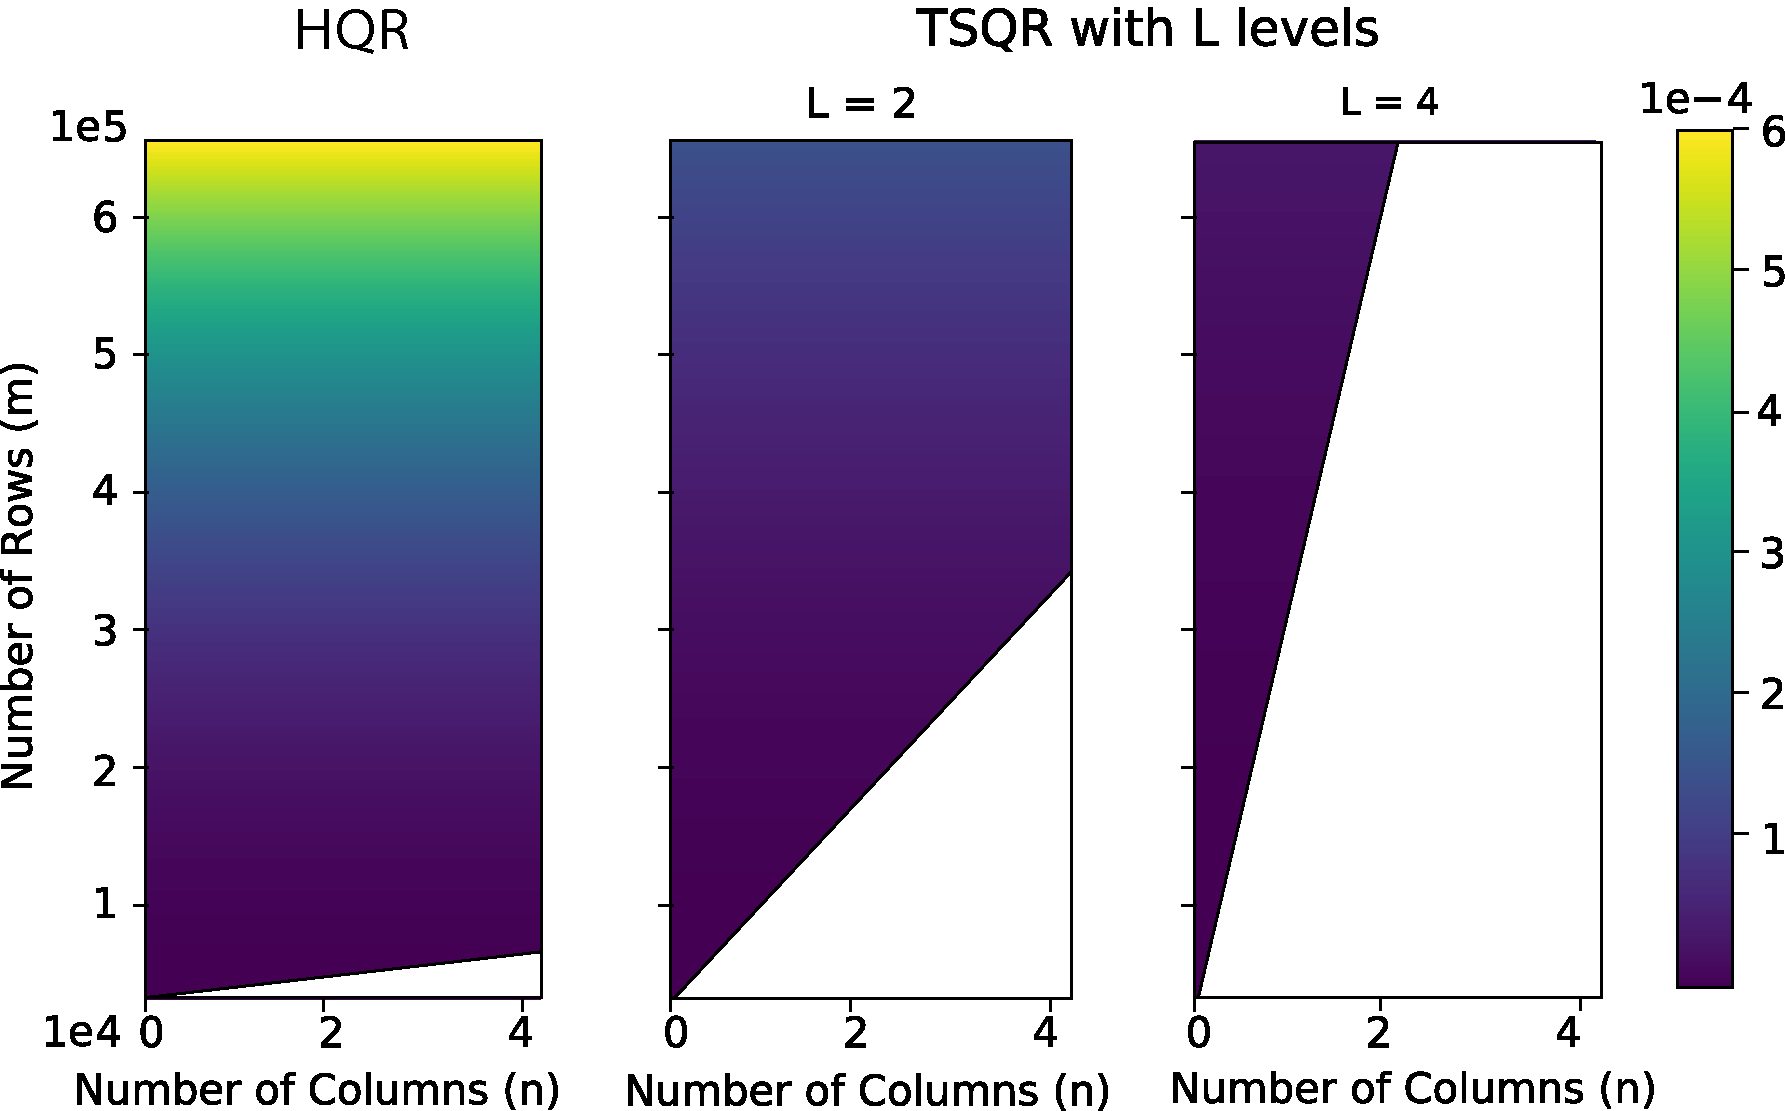
\includegraphics[width=.45\textwidth]{./figures/paramspace.png}
	\caption{\label{fig:paramspace} Non-white space indicates allowable matrix sizes for each scheme, and color map represents error bounds for $\|\bb{\Delta Q}\|_F$ for uniform precision error analysis when using double precision arithmetic.}
	\vspace{-10pt}	
\end{wrapfigure}
\section{Mixed precision error analysis}\label{sec:mpanalysis}
%Let us first consider rounding errors incurred from carrying out HQR in high precision, then cast down at the very end.
This could be useful in applications that require economical storage but have enough memory to carry out HQR in higher precision, or in block algorithms as will be shown in \cref{sec:mp-3,sec:mp-2}.
Consider two floating point types $\F_{l}$ and $\F_{h}$ where $\F_{l}\subseteq \F_{h}$, and for all $x,y\in\F_{l}$, the exact product $xy$ can be represented in $\F_{h}$.
Some example pairs of $\{\F_{l}, \F_{h}\}$ include $\{\text{fp16}, \text{fp32}\}$, $\{\text{fp32}, \text{fp64}\}$, and $\{\text{fp16}, \text{fp64}\}$.
Suppose that the matrix to be factorized is stored with low precision numbers, $\bb{A}\in\F_{l}^{m\times n}$.
Casting up adds no rounding errors, so we can directly apply the analysis that culminated in \cref{thm:feHQR}, and we only consider the columnwise forward error in the $\bb{Q}$ factor.
Then, the $j^{th}$ column of $\hat{\bb{Q}}_{HQR} = \bb{Q} + \Delta \bb{Q}_{HQR}$ is bounded normwise via $\|\Delta \bb{Q}_{HQR}[:,j]\|_2 \leq n\tilde{\gamma}_{m}^{h},$ and incurs an extra rounding error when $\bb{Q}\in\F_{h}^{m\times n}$ is cast down to $F_{l}^{m\times n}$.\par

First, consider casting down a higher precision number $x\in\F_h$ to $\F_l$ without overflow. 
We result in \[\text{\tt castdown}(x) = x(1+\dd^{(l)}),\;\; |\dd^{(l)}| < u^{(l)},\]
and accrues a single rounding error in the lower precision.
Extending this result, we represent the backward error of a casting down a vector in $\F_h^{(m)}$ with a linear transformation, $\bb{I}^{(l)}\in\R^{m\times m}$.
This transformation is a diagonal perturbation of the identity, $\bb{I}_m$.
For some vector $\bb{x}\in\F_h$, the cast down operation yields
\begin{equation}
	\bb{x}^{(l)} := \text{\tt castdown}(\bb{x}^{(h)}) = \bb{I}_{l}\bb{x}^{(h)} = (\bb{I}+\bb{E})\bb{x}^{(h)} = \bb{x}^{(h)}+\Delta \bb{x},
\end{equation}
where $|\Delta \bb{x}| \leq u^{(l)} |\bb{x}^{(h)}|$ and  $\|\Delta \bb{x}\|_2 \leq u^{(l)} \|\bb{x}^{(h)}\|_2$.
Then, $\bb{E} = \Delta \bb{x x}^{\top}/\|\bb{x}\|_2^2$ and we can use the same argument as in \cref{eqn:outer} to form a backward matrix norm bound, 
\begin{equation}
	\|\bb{E}\|_F\leq u^{(l)}. \label{eqn:castdown}
\end{equation}
Using this in \cref{lem:3.7} to analyze the forward norm error for the $j^{th}$ column of the $\bb{Q}$ factor computed with \cref{algo:hhQR} yields
\begin{equation}
	\|\text{\tt castdown}(\hat{\bb{Q}}_{HQR}[:,j]) - \bb{Q}[:,j]\|_2 = \|\bb{I}_l\hat{\bb{P}}_{1}\cdots\hat{\bb{P}}_{n}\hat{e}_j\|_2 \leq u^{(l)}+n\tilde{\gamma}_m^{(h)} + nu^{(l)}\tilde{\gamma}_m^{(h)}.\label{eqn:HQR-mp}
\end{equation}
%To convert this bound to the lower precision, we define function $d$,
%\begin{equation}
%d(m,u^{(h)}, q,u^{(l)}) := \lceil (qu^{(l)}+mu^{(h)})/u^{(l)}\rceil = \cO(q+mu^{(h)}/u^{(l)}),\label{eqn:d}
%\end{equation} 
%so that if $\|\hat{\bb{x}}-\bb{x}\|_2 \leq \gamma_m^{(h)}$, then $\|\text{\tt castdown}(\hat{\bb{x}})-\bb{x}\|_2 \leq \gamma_{d(m,u^{(h)}, q,u^{(l)})}^{(l)}$.
%This is a looser bound but it allows us to easily compare the errors to the uniform, low precision implementation of forming $\hat{\bb{x}}$.
%A looser upper bound is given by $\tilde{\gamma}_d^{(l)}$ where $d = \lceil u^{(l)}_+mu^{(h)}/u^{(l)}\rceil$ and we benefit from being able to represent it in terms of the low precision . 
%Additionally, we can use this to identify a function that allows us to formulate the new error bound after applying a castdown operation to vectors whose error bounds were known in high precision,
%Let $d = \lceil nmu^{(h)}/u^{(l)}\rceil$, so that $nmu^{(h)}\leq du^{(l)}$, and there exists some $r\leq \lfloor u^{(h)}/u^{(l)} \rfloor$ so that $nmu^{(h)} = (d-1)u^{(l)}+ru^{(h)}$.
%This $d$ value allows us to convert the error in terms of the higher precision to the lower precision while also adding in the extra rounding error that may be incurred in the casting down step. 
%Then, the componentwise error is bounded by
%\begin{equation}
%	|\text{{\tt castdown}}(\Delta \bb{Q}_{HQR}[i,j])| \leq \frac{cnmu^{(h)}}{1-cmu^{(h)}} \leq \frac{cdu^{(l)}}{1-cmu^{(h)}} \leq \tilde{\gamma}_{d}^{(l)},
%\end{equation}
%and the columnwise error is 
%\begin{equation}
%	\|\text{{\tt castdown}}(\Delta \bb{Q}_{HQR}[:,j])\|_2 \leq \left(\sum_{i=1}^m |\tilde{\tth}_d^{(l)}|^2 \right)^{1/2} \leq \sqrt{m}\gamma_d^{(l)}
%\end{equation}
%Since $\hat{\bb{Q}}_{HQR}$ should be almost orthogonal with respect to the higher precision, we can expect all components to be within the dynamic range of $\F_{l}$.
%In \ref{sec:mp-f}, we look at the rounding errors incurred from carrying out a QR factorization in a high precision, then cast down at the very end.
%Since this requires only one cast down operation, this is very similar to the results from the standard uniform precision analysis.
Similarly, we can apply the operator $\bb{I}^{(l)}$ to cast down any quantity stored in the higher precision. 
If BQR and TSQR were computed entirely in the higher precision then cast down at the end, then the corresponding forward matrix norm errors on the $\bb{Q}$ factor are
\begin{align*}
	\|\hat{\bb{Q}}_{BQR}\|_F&\leq u^{(l)}+n\tilde{\gamma}_m^{(h)} +u^{(l)}n\tilde{\gamma}_m^{(h)},\\
	%\leq \tilde{\gamma}_{d(nm,u^{(h)},u^{(l)})}^{(l)},\\
	\|\hat{\bb{Q}}_{TSQR}\|_F&\leq u^{(l)}+n(L\tilde{\gamma}_{2n}^{(h)}+\tilde{\gamma}_{m2^{-L}}^{(h)}) +u^{(l)}n(L\tilde{\gamma}_{2n}^{(h)}+\tilde{\gamma}_{m2^{-L}}^{(h)}).
	%\leq \tilde{\gamma}_{d(n(L2n+m2^{-L}),u^{(h)},1,u^{(l)})}^{(l)}.
\end{align*}

We will modify BQR and TSQR so that matrix-matrix multiply and accumulate operations can be performed on TensorCore block FMAs which work on $4$-by-$4$ matrices, $\bb{A},\bb{B},\bb{C},$, and $\bb{D}$ that compute \[
\bb{D} = \fl( \bb{C} +\bb{A}\bb{B}),\]
where $\bb{A},\bb{B}\in \F_{\text{fp16}}^{4\times 4}$ and  $\bb{C},\bb{D}\in \F_{\text{fp16}}^{4\times 4}$ or $\bb{C},\bb{D}\in \F_{\text{fp32}}^{4\times 4}$.
The inner product step in forming $\bb{A}\bb{B}$ is similar to \cref{assump:mp} in that full precision (exact) products are accumulated in the higher precision, fp32.
One difference is that the cast down operation at the end of the inner product is optional.
Matrices larger than $4$-by-$4$'s can be multiplied and added using this optional cast down feature and by using block matrix multiplication with $4$-by-$4$ blocks.
In \cref{sec:mp-3}, we consider performing BQR and TSQR with high precision FLOPs within a block/level, but cast down to low precision in between blocks and at the very end.
Finally, in \cref{sec:mp-2}, we consider all 3 algorithms with the ad hoc mixed precision setting described in \cref{assump:mp} where inner products are performed in high precision before being cast down, and all other operations are computed in low precision.
%\subsection{Round down at the end of the factorization}\label{sec:mp-f}
%Results in this section are quite straight forward, but 
%\subsubsection{HQR}
\subsection{Round down at block-level (BLAS-3)}\label{sec:mp-3}
We directly apply \cref{eqn:HQR-mp} to all instances of HQR to the error analyses for BQR and TSQR in \cref{sec:algo}.
Therefore, a cast down operation should occur at every block/level and the insertion of low precision errors $u^{(l)}$ should be somewhat correlated to the number of blocks and levels. 

\subsubsection{Round down at block level: BQR}\label{sec:mp-3b}
%Let us consider a setting in which only $M$ blocks of width $r$ can be loaded onto memory.
%Then, lines 2-6 of \cref{algo:blockHQR} can be modified via \cref{algo:mpBQR}.
%\begin{algorithm2e}
%	$q = N/M$\tcc*{Note that $n=Nr=qMr$.}
%	\For{$q'=1:q$}{
%		\If {$q'>2$} {
%				Update $[\bb{C}_{(q'-1)M+1}\cdots\bb{C}_{qM}]$ with WY updates from blocks $1:(q'-1)M$.
%		}
%		\For{$k=1:M$}{
%		Apply HQR to $\bb{C}_{(q'-1)M+k}$\;
%		Form WY update for $\bb{C}_{(q'-1)M+k}$\;
%		WY update blocks to the right, $[\bb{C}_{(q'-1)M+k+1}\cdots \bb{C}_{q'M}]$.
%	}
%}
%\caption{\label{algo:mpBQR} A portion of a mixed precision BQR: modifying first for-loop in \cref{algo:blockHQR}.}
%\end{algorithm2e}
%We now impose a mixed-precision setting where the inner for-loop in \cref{algo:mpBQR} is performed in high precision, but the WY updates for the outer loop is stored in low precision and only $M$ blocks is updated at a time due to the memory constraint.
%These low precision WY updates would be used to build the $\bb{Q}$ factor serially in groups of $M$.
Consider the input matrix, $\bb{A}\in\F_l^{m\times n}$, partitioned into $N$ blocks of $r$ columns, $\bb{A}=[\bb{C}_1 \cdots \bb{C}_N]$ as was in the analysis in \cref{sec:BQR}.
We assume that the returned factors should also be represented in the lower precision, $\F_l$, and modify \cref{algo:blockHQR} so that matrix-matrix multiply and accumulate operations are performed with TensorCore block FMAs.
Since approximately $\cO(1/N)$ (small) fraction of FLOPs are performed in level-1 and level-2 BLAS operations, we assume that we can afford to compute these in high precision.
Let us store the $\bb{R}$ factor from each call to HQR in low precision, and keep the Householder constants and vectors ($\bm{\beta}_k^{(j)}$,$\bb{v}_k^{(j)}$)in high precision to build the WY representation.
Since the WY representations ($\bb{W}_k$, $\bb{V}_k$) should be stored in low precision, we enforce a cast down at the end of \cref{algo:buildWY}.
Finally, all but the last WY update for each block are stored in the higher precision, and the last WY update returned in low precision. 
This mixed precision BQR variant is rich in level-3 BLAS operations can be implemented with TensorCore block FMAs easily, and is formally introduced in \cref{algo:mpBQR}.
\begin{algorithm2e}
	\DontPrintSemicolon % Some LaTeX compilers require you to use \dontprintsemicolon instead
	\KwIn{$\bb{A}\in\F_l^{m \times n}$, $r\in\R$ where $n=Nr$.}
	\KwOut{$\bb{Q}\in\F_l^{m \times n},\bb{R}\in\F_l^{n \times n}$}
	$N=\frac{n}{r}$\\
	\tcp{Let $\bb{A} = [\bb{C}_{1} \cdots  \bb{C}_{N}]$ where all blocks except $\bb{C}_{N}$ are $m$-by-$r$ sized.}
	%\tcp{Let $n_i=ri$ for $i=1:N-1$ and $n_N=n$.} 
	\For{$k=1:N-1$}{
		\If{$k == 1$}{
			$\bb{V}_{1},\bm{\beta}_1,\bb{C}_{1}\gets$ {\tt hhQR}({\tt castup}($\bb{C}_{k}$))\tcc*{\Cref{algo:hhQR} in high precision.}
		}
		\Else{
		$\bb{V}_{k},\bm{\beta}_k,\bb{C}_{k}\gets$ {\tt hhQR}($\bb{C}_{k}$)\tcc*{\Cref{algo:hhQR} in high precision.}	
	}
		$\bb{C}_{k}\gets ${\tt castdown }($\bb{C}_{k}$)\tcc*{Builds $\bb{R}$ factor in low precision.}
		%$\bb{V}_i,\bm{\beta}_i,\bb{A}_{n_{i-1}+1:m,n_{i-1}+1:n_i}\gets$ {\tt hhQR}$(\bb{A}_{n_{i-1}:m,n_{i-1}+1:n_i})$\tcc*{\Cref{algo:hhQR}}
		$\bb{W}_{k}\gets $ {\tt buildWY}$(\bb{V}_{k},\bm{\beta}_k)$ \tcc*{\Cref{algo:buildWY} in high precision}
		$[\bb{V}_{k},\bb{W}_{k}]\gets ${\tt castdown}($[\bb{V}_{k},\bb{W}_{k}]$)\;
		$[\bb{C}_{k+1}\cdots\bb{C}_{N}]$ -= $\bb{V}_{k} \left(\bb{W}_{k}^{\top}[\bb{C}_{k+1}\cdots\bb{C}_{N}]\right) $ \tcc*{returned in low precision}
	}
	\tcp{Now build $\bb{Q}$ using level-3 BLAS operations.} 
	$\bb{Q}\gets \bb{I}$\tcc*{$\bb{I}_m$ if full QR, and $\bb{I}_{m\times n}$ if thin QR.}
	\For{$k=N:-1:1$}{
		\tcp{All updates are returned in low precision.}
		$\bb{Q}[(k-1)r+1:m,(k-1)r+1:n]$-= $\bb{W}_k \left(\bb{V}_k^{\top}\bb{Q}[(k-1)r+1:m,(k-1)r+1:n]\right)$
	}
	%\tcp{The last update is returned in low precision.}
	%$\bb{Q}$-= $\bb{W}_1 \left(\bb{V}_1^{\top}\bb{Q}\right)$\;
	\Return $\bb{Q},\bb{A}$
	\caption{\label{algo:mpBQR} $\hat{\bb{Q}}_{mpBQR},\hat{\bb{R}}_{mpBQR}\gets {\tt mpBQR}(\bb{A}, r)$: Perform Householder QR factorization of matrix $\bb{A}$ with column partitions of size $r$. All inputs and outputs are stored in low precision. Matrix-matrix multiplication and accumulate operations in lines 10, 13, and 14 require low precision inputs but can return in either of the two precisions.}
\end{algorithm2e}


Since $\hat{\bb{W}}_{k},\hat{\bb{Y}}_k$'s are computed with \cref{algo:buildWY} then cast down, the low precision WY update is $\hat{\bb{X}}_{k}^{(l)} = \bb{I}-\bb{I}^{(l)}\hat{\bb{W}}_k\bb{I}^{(l)}\hat{\bb{V}}_k^{(\top)}$.
Consider applying $\hat{\bb{X}}_k^{(l)}$ to some matrix stored in low precision, $\bb{B}$ using the TensorCore block FMAs.
We analyze a single column $\bb{b}_j:=\bb{B}[:,j] \in \F_l^{m-(k-1)r}$ even though this operation is done on $\bb{B}$ as a whole.
Let $\bb{I}^{(l)}\hat{\bb{W}}_k = \hat{\bb{W}}_k + \bb{E}_W\hat{\bb{W}}_k$ and $\bb{I}^{(l)}\hat{\bb{W}}_k = \hat{\bb{Y}}_k + \bb{E}_Y\hat{\bb{Y}}_k$, where $|\bb{E}_W|,|\bb{E}_Y| \leq u^{(l)}$ componentwise.  
Since \[\hat{\bb{X}}_{k}^{(l)}- \bb{X}_k = \hat{\bb{X}}_{k}^{(l)} -\hat{\bb{X}}_{k}+ \hat{\bb{X}}_{k}- \bb{X}_k= \hat{\bb{X}}_{k}^{(l)} -\hat{\bb{X}}_{k}+ \Delta \bb{X}_{k},\]
we only need to add the errors introduced from casting down to the errors derived in \cref{eqn:deltX},
\begin{align*}
	\|(\hat{\bb{X}}_{k}^{(l)}- \hat{\bb{X}}_{k}+ \Delta \bb{X}_{k})\bb{b}_j \|_2 %&=\| (\bb{b}_j-(\hat{\bb{W}}_k + \bb{E}_W\hat{\bb{W}}_k)((\hat{\bb{Y}}_k + \bb{E}_Y\hat{\bb{Y}}_k)^{\top}\bb{b}_j)) - (\bb{b}_j-\hat{\bb{W}}_k(\hat{\bb{Y}}_k^{(\top)}\bb{b}_j) + \Delta \bb{X}_{k} \bb{b}_j\|_2\\
	&= \| \left(-\left(\bb{E}_W+\bb{E}_Y+ \bb{E}_W\bb{E}_Y\right)\hat{\bb{W}}_k\hat{\bb{Y}}_k^{\top} + \Delta \bb{X}_{k} \right)\bb{b}_j\|_2,\\
	&= (\gamma_2^{(l)}(1+r\tilde{\gamma}_{m-(k-1)r}^{(h)}) + r\tilde{\gamma}_{m-(k-1)r}^{(h)}) \|\bb{b}_j\|_2.
%	\text{\tt castdown}(\hat{\bb{P}}_{k'}^{(1)}\cdots\hat{\bb{P}}_{k'}^{(r)}) \\
%	\|\hat{\bb{X}}_{k'} - \bb{X}_{k'}\|_F &= \|\bb{I}^{(l)}\hat{\bb{P}}_{k'}^{(1)}\cdots\hat{\bb{P}}_{k'}^{(r)} -\bb{P}_{k'}^{(1)}\cdots\bb{P}_{k'}^{(r)} \|_F \leq (1+u^{(l)})(1+r\tilde{\gamma}_{m-(k'-1)r})-1,
\end{align*}
Therefore, we have $\|(\hat{\bb{X}}_k^{(l)}-\bb{X}_k)\bb{b}_j\|_2 \leq (\gamma_2^{(l)} +r\tilde{\gamma}_{m-(k-1)r}^{(h)} + r\gamma_2^{(l)}\tilde{\gamma}_{m-(k-1)r}^{(h)}) \|\bb{b}_j\|_2 $ and the error bound on the corresponding backward matrix norm is

\begin{equation}
	\|\Delta^{(l)}\bb{X}_k\|_F \leq \gamma_2^{(l)} +r\tilde{\gamma}_{m-(k-1)r}^{(h)} + r\gamma_2^{(l)}\tilde{\gamma}_{m-(k-1)r}^{(h)},\label{eqn:mpdeltX}
\end{equation}
where $\Delta^{(l)}\bb{X}_k = \hat{\bb{X}}_k^{(l)}-\bb{X}_k$.

We can finally compute the forward errors on the QR factorization computed via \cref{algo:mpBQR}.
Consider the $j^{th}$ column of the $\bb{Q}$ factor, which we denote with $\bb{q}_j:=\hat{\bb{Q}}_{mpBQR}[:,j]$, and let $k = \lfloor j/r\rfloor$.
for $k'=1:N$, and \cref{eqn:mpdeltX} was used to invoke \cref{lem:3.7}.
Then the columnwise error is 
\begin{align}
	\|\Delta \bb{q}_j \|_2 &\leq -1 + \prod_{k'=1}^k (1+\gamma_2^{(l)})(1+r\tilde{\gamma}_{m-(k'-1)r}^{(h)})\\ 
	&\leq k\gamma_{2}^{(l)} + kr\tilde{\gamma}_m^{(h)} + k^2r\gamma_{2}^{(l)}\tilde{\gamma}_m^{(h)}, \label{eqn:mpBQRcol}
\end{align} 
where $\Delta \bb{q}_j = (\hat{\bb{X}}_1^{(l)}\cdots\hat{\bb{X}}_k^{(l)} - \bb{X}_1\cdots\bb{X}_k )\hat{e}_j.$
Summing over the columns to find a matrix norm error bound yields
\begin{equation}
	\|\hat{\bb{Q}}_{mpBQR}-\bb{Q}\|_F \leq n^{1/2}\tilde{\gamma}_{N}^{(l)} + n^{(3/2)}\tilde{\gamma}_m^{(h)},
\end{equation}
where the summation of the third term in \cref{eqn:mpBQRcol} is swept under the tilde notation in $n^{1/2} \tilde{\gamma}_{N}^{(l)}$.
This bound shows that \cref{algo:mpBQR} only adds $n^{1/2}\tilde{\gamma}_{N}^{(l)}$ order errors to the bounds in \cref{eqn:BQRmat}.
Using that $u^{(l)}=M_{l,h}u^{(h)}$, this increase corresponds to a multiplicative factor shown below,
\begin{equation}
	n^{1/2}\tilde{\gamma}_{N}^{(l)} + n^{(3/2)}\tilde{\gamma}_m^{(h)} \approx \left(1+\frac{M_{l,h}}{rm}\right)n^{(3/2)}\tilde{\gamma}_m^{(h)}. \label{eqn:mpBQR3}
\end{equation}
Therefore, the loss in accuracy due to mixed precision computing is relatively small when the disparity in precision ($M_{l,h}$) is small in comparison to the block size, $mr$.
Whether this loss in accuracy in the worst-case scenario is worth the speed-ups from using mixed precision hardware is an open question that can be tackled in future research.
We expect that the block size $r$, the dimension of the input matrix $m,n$, and hardware specificities will be contributing factors. 

\subsubsection{Round down at block level: TSQR}\label{sec:mp-3t}
%Unlike BQR, which is rich in level-3 BLAS operations, TSQR d
%Since the majority of FLOPs in BQR use level-3 BLAS operations, it was simple to adapt TensorCore block FMAs within the algorithm.
%
%TSQR is best suited for tall-and-skinny matrices where $m\gg n$. 
%The majority of the computational gains are from parallelizing the QR factorizations of the initial level blocks, which are performed by different node/tasks ideally.
Let us now consider a variant of TSQR, where all instances of {\tt hh\_mult} are replaced by some level-3 BLAS operations.
Note that for all blocks in all levels, exactly $n$ Householder transformations of lengths either $m2^{-L}$ or $2n$ are applied via {\tt hh\_mult}.
Let $\tilde{m} := \max\{m2^{-L},2n\}$ be the larger of the two. 
We consider two ways of applying $n$ Householder transformations with level-3 BLAS operations.
\begin{enumerate}
	\item Consider building the WY representation using high precision arithmetic, casting them down and then applying the update with TensorCore block FMAs.
	The multiplication by the $\bb{Y}$ factor requires at most $\tilde{m}$-length inner products and a cast down operation and the multiplication by the $\bb{W}$ factor requires $n$-length inner products and another cast down operation.
	The errors accumulated from these actions are bounded by $\cO(3u^{(l)}+\tilde{\gamma}_{\tilde{m}n}^{(h)})$ componentwise.
	\item Now, consider applying the $n$ Householder transformations by forming the operator explicitly then computing a single matrix-matrix product.
	We form the operator using the same steps as forming the $\bb{Q}$ factor in HQR in high precision arithmetic, then cast the result down. 
	The construction of the operator and the cast down result in error bounded by $\cO(u^{(l)}+\tilde{\gamma}_{\tilde{m}n}^{(h)})$, and the matrix-matrix product requires $\tilde{m}$-length inner products and another cast down operation. 
	This option also accrues error bounded by $\cO(2u^{(l)}+\tilde{\gamma}_{\tilde{m}n}^{(h)})$.
\end{enumerate}

Both of these options require more FLOPs than in the standard algorithm implemented with level-2 BLAS operations, since the same number of level-2 BLAS operations are required to form the matrices required for the level-3 variants. 
The level-3 variants are built during the formation of the $\bb{R}$ factor and can be reused when forming the $\bb{Q}$ factor.
Notice that unlike BQR which is rich in level-3 BLAS operations by design, it is not clear whether implementing TSQR with level-3 BLAS operations has obvious benefits.
Regardless, we still perform a rounding error analysis of TSQR performed with mixed precision level-3 BLAS operations, i.e. TensorCore block FMAs.

The analysis in \cite{Mori2012} shows that each column of $\bb{Q}$ is transformed by $n$ Householder transformations of length $2n$ from levels $L:-1:1$, and another set of $n$ Householder transformations of length $m2^{-L}$ at level $0$.
We can easily modify the analysis in \cite{Mori2012} and applying \cref{lem:3.7} by adding $(1+2u^{(l)})$ to every set of $n$ Householder transformations in each level.
There are two low precision rounding errors in each block per level since casting down the matrix operator formed with high precision is cast down to the low precision, and the matrix-matrix product used in applying this operator with TensorCore block FMAs incurs another low precision rounding error. 
Therefore, all instances of $n\tilde{\gamma}_{m2^{-L}},n\tilde{\gamma}_{2n}$ are replaced with \[(1+2u^{(l)})(1+n\tilde{\gamma}_{m2^{-L}}^{(h)})-1,\quad\text{and}\quad (1+2u^{(l)})(1+n\tilde{\gamma}_{2n}^{(h)})-1.\]
Then, the $\bb{Q}$ factor formed with this mixed precision variant of TSQR is denoted with $\hat{\bb{Q}}_{mpTSQR}$ and its $j^{th}$ column has rounding errors bounded by,
\begin{equation}
\|\hat{\bb{Q}}_{mpTSQR}[:,j] - \bb{Q}[:,j]\|_2 \leq \tilde{\gamma}_{L+1}^{(l)}+n\left(L\tilde{\gamma}_{2n}^{(h)}+\tilde{\gamma}_{m2^{-L}}^{(h)}\right)\label{eqn:mpTSQR1}.
\end{equation}
Summing up the columns for a matrix norm error bound, we result in 
\begin{equation}
	\|\hat{\bb{Q}}_{mpTSQR} - \bb{Q}\|_F \leq n^{1/2}\tilde{\gamma}_{L+1}^{(l)}+n^{3/2}\left(L\tilde{\gamma}_{2n}^{(h)}+\tilde{\gamma}_{m2^{-L}}^{(h)}\right).\label{eqn:mpTSQR2}
\end{equation}
Therefore, we can convert the additional low precision rounding errors into a multiplicative factor of the original bound in \cref{eqn:tsqrQ},
\begin{equation}
	n^{1/2}\tilde{\gamma}_{L+1}^{(l)}+n^{3/2}\left(L\tilde{\gamma}_{2n}^{(h)}+\tilde{\gamma}_{m2^{-L}}^{(h)}\right) = (1+ \frac{M_{l,h}L}{n(2nL+m2^{-L})})n^{3/2}\left(L\tilde{\gamma}_{2n}^{(h)}+\tilde{\gamma}_{m2^{-L}}^{(h)}\right).
\end{equation}
Once again, the constant that represents the disparity in the two precisions, $M_{l,h}$ is compared against the original matrix size $m,n$ and the block size specifications defined by $2^{L}$ and the number of levels, $L$.
%TODO: conclusion maybe a parameter regime analysis for m, n, L, M?
%Let us now consider a WY variant of TSQR, where all instances of {\tt qr} (lines 6,7,9 of \cref{algo:par_tsqr}) are followed by {\tt buildWY} (see \cref{algo:buildWY}), and all instances of {\tt hh\_mult} is replaced by a WY update (line 6 of \cref{algo:blockHQR}).
%We additionally impose a mixed precision assumption similar to \cref{sec:mp-3b}, where we store all WY representations of HQR within the for-loop (lines 4-8) of \cref{algo:par_tsqr} in low precision, and consider the construction of the $\bb{Q}$ factor.
%We can assume that each $2n$-by-$n$ and $m2^{-L}$-by-$n$ size matrices can fit into memory and only introduce one cast down for each $\bb{Q}_j^{(i)}$ block, where $i=1:L-1$ and $j=1:2^{i-1}$.
%Let us compute lines 9-10 in the higher precision, which introduces an error of order $n\tilde{\gamma}_{2n}^{(h)}$.
%In levels $L-1$ to $1$, each WY update adds error $u^{(l)}+n\tilde{\gamma}_{2n}^{(h)}$, and the final construction at the $0^{th}$ level (line 16), the WY update adds error $u^{(l)} + n\tilde{\gamma}_{m2^{-L}}^{(h)}$.

\subsection{Round down at inner-product}\label{sec:mp-2}
While the previous section discussed blocked variants of HQR that can be easily adapted for the mixed precision setting specific to TensorCore's level-3 BLAS operations, we want to provide a more general mixed precision environment in this section.
Recall that HQR, BQR, and TSQR all rely on Householder transformations in one way or another, and Householder transformations are essentially performed via \cref{eqn:effH}.
This implementation capitalizes on the rank-1 update structure of Householder transformations where the predominant share of FLOPs is spent on an inner product, and computing the Householder vector and constant also rely heavily on inner products.
Therefore, we can attribute nearly all of the computational tasks for \cref{algo:hhQR,algo:blockHQR,algo:par_tsqr} to the inner product.
In addition, the inner product is just as important in non-HQR linear algebra tools, where some examples include projections and matrix-vector, matrix-matrix multiply.
Consequently, we return to the mixed precision setting described in \cref{sec:background}, where every inner product is cast down to the lower precision as shown in \cref{eqn:aftercd}.
\subsubsection{Round down at inner product: HQR}
Consider forming a Householder transformation that zeros out $\bb{x}\in\R^m$ below the the $i^{th}$ element. 
We need to compute $\sigma$, $\beta$, $\tilde{\bb{v}}_1$, and $\bb{v}$ as defined in \cref{sec:HQR}:
\begin{align}
\fl(\sigma) &= \rm{fl}(-\rm{sign}(\bb{x}[1])\|\bb{x}\|_2) = \sigma + \Delta \sigma,\;\;|\Delta\sigma| \leq (\gamma_{2}^{(l)}+\gamma_{m}^{(h)}+\gamma_{2}^{(l)}\gamma_{m}^{(h)})|\sigma|,\label{eqn:mpsigma}\\
\fl(\bb{\tilde{v}}[1])& =\bb{\tilde{v}}[1] + \Delta \bb{\tilde{v}}[1] = (1+\dd^{(l)}) (\bb{x}[1]-\sigma-\Delta\sigma), \;\;|\Delta\bb{\tilde{v}}[1]| \leq (\gamma_{3}^{(l)}+\tilde{\gamma}_{m}^{(h)})|\bb{\tilde{v}}[1]| \label{eqn:mpv1}\\
\fl(\beta) &= \beta +\Delta \beta= (1+\dd^{(l)})\left(-\tilde{\bb{v}}[1]/\hat{\sigma}\right), \;\; |\Delta\beta| \leq (\gamma_{8}^{(l)}+\tilde{\gamma}_{m}^{(h)})|\beta|, \label{eqn:mpbeta}
\end{align}
\begin{equation}
	\fl(\bb{v}[j])	= \bb{v}[j] + \Delta \bb{v}[j]\text{ where }|\Delta \bb{v}_j|\leq 
	\begin{cases}
	0,& j=1\\
	(\gamma_{7}^{(l)} + \tilde{\gamma}_{m}^{(h)})|\bb{v}_j|,&j=2:m-i+1.
	\end{cases}  \label{eqn:mpv}
\end{equation}
These bounds on $\Delta\sigma$, $\Delta \bb{\tilde{v}}[1]$, $\Delta \beta$, and $\Delta \bb{v}[j]$ are computed by using the rules from \cref{lem:mp} on the analysis shown in \cref{sec:HQR}.
Using these, we can formulate the mixed precision version of \cref{eqn:applyP} where $\hat{\bb{y}}=\fl(\bb{P_vx})\in\R^m$ is implemented via \cref{eqn:effH}.
Note that the inner product $\hat{\bb{v}}^{\top}\bb{x}$ is computed with the mixed precision inner product scheme outlined in \cref{assump:mp}, and all other operations are done in the lower precision.
Then, the transformed vector is bounded by
\begin{equation}
	\hat{\bb{y}} = \bb{y}+\Delta \bb{y},\;\; \|\Delta \bb{y}\|_2 \leq (\gamma_{25}^{(l)} + \tilde{\gamma}_{m}^{(h)})\|\bb{y}\|_2.\label{eqn:mpdelty}
\end{equation}
Thus, a backward error can be formed using $\Delta \bb{P_v} = \Delta \bb{y}\bb{x}^{
\top}/\|\bb{x}\|_2^2$,
\begin{equation}
	\hat{\bb{y}} = (\bb{P_v} + \Delta \bb{P_v})\bb{x},\;\; \|\Delta \bb{P_v}\|_F\leq (\gamma_{25}^{(l)} + \tilde{\gamma}_{m}^{(h)}). \label{eqn:mpapplyP}
\end{equation}
Now, we form the error bounds for applying $n$ Householder transformations to $\bb{x}$ using \cref{lem:3.7},
\begin{align}
\hat{\bb{y}} &= \bb{Q} (\bb{x} +\Delta \bb{x}) = (\bb{Q} + \Delta \bb{Q})\bb{x},\\
\|\Delta \bb{y}\|_2 &\leq (\tilde{\gamma}_n^{(l)}+n\tilde{\gamma}_m^{(h)})\|\bb{x}\|_2,\;\; \|\Delta \bb{Q}\|_F\leq (\tilde{\gamma}_n^{(l)}+n\tilde{\gamma}_m^{(h)}).\label{eqn:mp19.3}
\end{align} 
Note that we have additionally assumed that $25 \ll n$ and used the $\tilde{\gamma}^{(l)}$ notation.
The analogous mixed precision QR factorization error bounds are shown in \cref{thm:mpHQR}.
\begin{theorem}
	\label{thm:mpHQR}
	Let $\bb{A}\in\R^{m\times n}$ with $m\geq n$ have full rank, $n$. 
	Let $\hat{\bb{Q}}_{mpHQR}\in\R^{m\times n}$ and $\hat{\bb{R}}\in\R^{n\times n}_{mpHQR}$ be the thin QR factors of $\bb{A}$ obtained via \cref{algo:hhQR} with mixed precision FLOPs where inner products are computed in precision $h$ then cast down.
	All other operations are carried out in precision $l$.
	Then,
	\begin{align*}
%	\hat{\bb{R}} &= \bb{R} + \Delta \bb{R}__{mpHQR} = \fl(\hat{\bb{P}}_n\cdots\hat{\bb{P}}_1 \bb{A}),\\
%	\hat{\bb{Q}} &= \bb{Q} + \Delta \bb{Q} = \fl(\hat{\bb{P}}_1\cdots\hat{\bb{P}}_n \bb{I}),\\
	\|\Delta \bb{R}_{mpHQR}[:,j]\|_2&\leq (\tilde{\gamma}_n^{(l)}+n\tilde{\gamma}_m^{(h)}) \|\bb{A}[:,j]\|_2,\;\; \|\Delta \bb{R}_{mpHQR}\|_F\leq (\tilde{\gamma}_n^{(l)}+n\tilde{\gamma}_m^{(h)}) \|\bb{A}\|_F\\
	\|\Delta \bb{Q}[:,j]_{mpHQR}\|_2&\leq (\tilde{\gamma}_n^{(l)}+n\tilde{\gamma}_m^{(h)}),\;\; \|\Delta \bb{Q}_{mpHQR}\|_F \leq n^{1/2} (\tilde{\gamma}_n^{(l)}+n\tilde{\gamma}_m^{(h)}).
	\end{align*}
%	Let $\bb{A}+\Delta \bb{A} = \hat{\bb{Q}}\hat{\bb{R}}$, where $\hat{\bb{Q}}$ and $\hat{\bb{R}}$ are obtained via Algorithm~\ref{algo:hhQR}.
%	Then the backward e|rror is
%	\begin{equation}
%	\|\Delta \bb{A}\|_F \leq n^{3/2}\tilde{\gamma}_{m}\|\bb{A}\|_F.
%	\end{equation}
\end{theorem}

%TODO: what do these bounds mean?

\subsubsection{Round down at inner product: BQR}
Now, we analyze \cref{algo:blockHQR} with the mixed precision inner product scheme of \cref{assump:mp}. 
At the $k^{th}$ block, we first apply the mixed precision HQR summarized in \cref{thm:mpHQR}.
Next, we construct the WY representation, where we can now use \cref{eqn:mpdelty,eqn:mpapplyP,lem:3.7} to form
\begin{equation}
	\|\hat{\bb{X}}_{k}^{(l)}- \bb{X}_k\|_F = \|(\hat{\bb{P}}_k^{(1)}\cdots \hat{\bb{P}}_k^{(r)})-(\bb{P}_k^{(1)}\cdots \bb{P}_k^{(r)}))\|_F \leq \tilde{\gamma}_{r}^{(l)} + r\tilde{\gamma}_{m}^{(h)}.
\end{equation}
Then, the $j^{th}$ column of the $\bb{Q}$ factor resulting from this mixed precision variant of BQR incurs rounding errors bounded by
\begin{equation}
	\|\hat{\bb{Q}}_{mpBQR2}[:,j]\|_F = \|\hat{\bb{X}}_1\cdots\hat{\bb{X}}_N\hat{e}_j\|_2\leq N\tilde{\gamma}_{r}^{(l)} + n\tilde{\gamma}_{m}^{(h)},
\end{equation}
and the matrix norm error bound is, 
\begin{equation}
	\|\hat{\bb{Q}}_{mpBQR2}\|_F \leq n^{1/2}N\tilde{\gamma}_{r}^{(l)} + n^{3/2}\tilde{\gamma}_{m}^{(h)} \approx (1+\frac{M_{l,h}}{m})n^{3/2}\tilde{\gamma}_{m}^{(h)}. \label{eqn:mpBQR2}
\end{equation}
Recall that the block mixed precision variant of \cref{sec:mp-3b} yielded a multiplicative factor of $(1+\frac{M_{l,h}}{rm})$ (see \cref{eqn:mpBQR3}).
This implies that the mixed precision inner product introduces low precision error $r\times $ larger than the low precision errors incurred from casting down at the block level.
However, if $m$ is sufficiently larger than $M_{l,h}$, the mixed precision inner product can still had non-leading order error terms to the worst-case scenario.
\subsubsection{Round down at inner product: TSQR}
Finally, we consider using the mixed precision inner product of \cref{assump:mp} in \cref{algo:par_tsqr}.
This corresponds to replacing every instance of $n\tilde{\gamma}_{m'}$ for $m'\in\{2n, m2^{-L}\}$ in \cref{thm:moriTSQR} with $\tilde{\gamma}_n^{(l)} + n\tilde{\gamma}_{m'}^{(h)}$.
We first consider the norm errors for the $j^{th}$ column of the $\bb{Q}$ factor computed by this mixed precision variant of \cref{algo:par_tsqr},
\begin{equation}
	\|\hat{\bb{Q}}_{mpTSQR2}[:,j] -\bb{Q}[:,j]\|_2 \leq (L+1)\tilde{\gamma}_n^{(l)} +n(\tilde{\gamma}_{m2^{-L}}^{(h)} + L\tilde{\gamma}_{ 2n}^{(h)}).\label{eqn:mptsqr2Qcol}
\end{equation} 
Then, the matrix norm error bound is 
\begin{align}
\|\hat{\bb{Q}}_{mpTSQR2}-\bb{Q}\|_F \leq n^{1/2}(L+1)\tilde{\gamma}_n^{(l)} +n^{3/2}(\tilde{\gamma}_{m2^{-L}}^{(h)} + L\tilde{\gamma}_{ 2n}^{(h)})\\
\approx \left(1+ \frac{M_{l,h}L}{m2^{-L}+ 2Ln}\right)n^{3/2}(\tilde{\gamma}_{m2^{-L}}^{(h)} + L\tilde{\gamma}_{ 2n}^{(h)}).\label{eqn:mptsqr2Q}
\end{align} 
%TODO: conclude
In this section, we consider three different mixed precision settings for the QR factorization, all of which take in a matrix $\bb{A}$ stored in low precision and return $\bb{Q},\bb{R}$ both represented in low precision. 
First, we consider a trivial mixed precision setting where HQR, BQR, and TSQR are computed in high precision after casting up the input matrix at the beginning, and casting down the resulting high precision factors to low precision. 
Then in \cref{sec:mp-3}, we modify BQR and TSQR to utilize level-3 BLAS operations and TensorCore bFMAs for the matrix product subroutines. 
Finally, we impose \cref{assump:mp} in \cref{sec:mp-2} to see how a mixed precision inner product impacts HQR, BQR, and TSQR when applied in level-2 BLAS operations.

\paragraph{Backward error of casting down vectors} First, consider
casting down a vector  $\bb{x}\in\F_h^{(m)}$.
The componentwise forward error is, \[\text{\tt castdown}_{l}(\bb{x}) = \bb{x} + \Delta {\bb{x}},\;\; |\Delta\bb{x}| < u^{(l)}|\bb{x}|.\]
We use this to represent the backward error of a casting down a vector with a linear transformation, $\bb{I}^{(l)}:=\bb{I} +\bb{E}\in\R^{m\times m}$, a diagonal perturbation of the identity.
We write,
\begin{equation}
\bb{x}^{(l)} := \text{\tt castdown}(\bb{x}^{(h)}) = \bb{I}^{(l)}\bb{x}^{(h)} = (\bb{I}+\bb{E})\bb{x}^{(h)} = \bb{x}^{(h)}+\Delta \bb{x},
\end{equation}
where $|\Delta \bb{x}| \leq u^{(l)} |\bb{x}^{(h)}|$ and  $\|\Delta \bb{x}\|_2 \leq u^{(l)} \|\bb{x}^{(h)}\|_2$.
Thus, $\bb{E} = \Delta \bb{x x}^{\top}/\|\bb{x}\|_2^2$ and we can use the same argument as in \cref{eqn:outer} to form a backward matrix norm bound, 
\begin{equation}
\|\bb{E}\|_F\leq u^{(l)}. \label{eqn:castdown}
\end{equation}

\paragraph{Casting down after HQR in high precision} Let us consider the trivial case of carrying out HQR in high precision and casting down at the very end.
This is useful for the analysis of mixed precision
block algorithms as will be shown in \cref{sec:mp-3}.
If the two floating point types $\F_{l}$ and $\F_{h}$ satisfy $\F_{l}\subseteq \F_{h}$
and the matrix to be factorized is stored with low precision numbers, $\bb{A}\in\F_{l}^{m\times n}$, then casting up adds no rounding errors.
Therefore, we can directly apply the analysis that culminated in \cref{thm:feHQR}, and we only consider the columnwise forward error in the $\bb{Q}$ factor.
Then, the $j^{th}$ column of $\hat{\bb{Q}}_{HQR} = \bb{Q} + \Delta \bb{Q}_{HQR}$ is bounded normwise via $\|\Delta \bb{Q}_{HQR}[:,j]\|_2 \leq n\tilde{\gamma}_{m}^{h},$ and incurs an extra rounding error when $\hat{\bb{Q}}_{HQR}\in\F_{h}^{m\times n}$ is cast down to $\F_{l}^{m\times n}$.
Using this in \cref{lem:3.7} to analyze the forward norm error for the $j^{th}$ column of the $\bb{Q}$ factor computed with \cref{algo:hhQR} yields
\begin{equation}
	\|(\text{\tt castdown}(\hat{\bb{Q}}_{HQR})- \bb{Q})[:,j]\|_2 = \|(\bb{I}^{(l)}\hat{\bb{P}}_{1}\cdots\hat{\bb{P}}_{n}-\bb{P}_{1}\cdots\bb{P}_{n})\hat{\bb{e}}_j\|_2 \leq u^{(l)}+n\tilde{\gamma}_m^{(h)} + nu^{(l)}\tilde{\gamma}_m^{(h)}.\label{eqn:HQR-mp}
\end{equation}
The final castdown operation increases the upper bound by $u^{(l)}$ and the size of $\bb{A}$ has no impact on this extra rounding error.
Applying this trivial mixed precision setting to BQR and TSQR would simply increases the error bound by approximately $u^{(l)}$ all the while taking an even longer time than the high precision implementation due the extra cast down and cast up operations.
Therefore, we do not analyze the rounding error analysis of this mixed precision variant of BQR and TSQR.
However, we will use this mixed precision HQR as a subroutine of the mixed precision BQR and TSQR in the following section.
%\subsection{Round down at block-level: level-3 BLAS mixed precision setting}\label{sec:mp-3}
The mixed precision setting in this section is designed to meet the below requirements.
\begin{enumerate}
	\item Modify \Cref{algo:blockHQR,algo:par_tsqr} to maximize level-3 BLAS operations and use TensorCore bFMAs. 
	\item Apply \cref{eqn:HQR-mp} to all instances of HQR to the error analyses for BQR and TSQR in \cref{sec:algo}.
	\item Cast down quantities at every block/level and the insertion of low precision errors $u^{(l)}$ should be somewhat correlated to the number of blocks and levels. 
	\item Both input and output of the various QR factorization algorithms are given in the low precision. 
\end{enumerate}
TensorCore's bFMA computes 
\begin{equation}
\hat{\bb{D}} =\fl_{TC}(\bb{C} + \bb{A}\bb{B}),\qquad \bb{C},\bb{D}\in\F_{\text{fp16}}^{4\times 4}\text{ or }\F_{\text{fp32}}^{4\times 4},\text{ and } \bb{A},\bb{B}\in\F_{\text{fp16}}^{4\times 4},\label{eqn:bFMA}
\end{equation}
and employs \emph{full} precision products and fp32 summation accumulate.
Here, the \emph{full} precision multiplication is exact as explained in \cref{sec:background}.
In \cite{Blanchard2019}, the authors investigate all four possible matrix-matrix multiplication routines in TensorCore, which depend on whether $\bb{C}$ and $\bb{D}$ are computed in fp16 or fp32. 
They also note that matrices larger than $4$-by-$4$ can still be computed using this block FMA by accumulating matrix sums with $\bb{C}\in\F_{\text{fp32}}^{4\times 4}$.
Suppose that we aim to compute a fp16 matrix product of two fp16 matrices, $\bb{X}\in\F_{(fp16)}^{m\times p}$, $\bb{Y}\in\F_{(fp16)}^{p\times n}$, and $\bb{Z}=\bb{XY}\in\F_{\text{fp16}}^{m\times n}$.
We pad $\bb{X},\bb{Y}$ with zeros so that all matrix dimensions are multiples of $4$ and the matrix product can be computed with the TensorCore block FMA.
Let $\bb{Q}_{[i,j]}:= \bb{Q}[4(i-1)+1:4i,4(j-1)+1:4j]$ refer to the $(i,j)^{th}$ $4$-by-$4$ block for any $\bb{Q}\in\{\bb{X},\bb{Y},\bb{Z}\}$.
Then, we compute $\bb{Z}_{[i,j]}$ via \[
\bb{Z}_{[i,j]} = \sum_{k=1}^{\lceil p/4\rceil} \bb{X}_{[i,k]} \bb{Y}_{[k,j]},
\]
where we use \cref{eqn:bFMA} by initializing with $\bb{A}^{(1)}:= \bb{X}_{[i,1]}$, $\bb{B}^{(1)}:= \bb{Y}_{[1,j]}$, and $\bb{C}^{(1)}:= \bb{0}_{4\times 4}$ and setting $\bb{A}^{(k)}:= \bb{X}_{[i,k]}$, $\bb{B}^{(k)}:= \bb{Y}_{[k,j]}$, and $\bb{C}^{(k)}:= \bb{D}^{(k-1)}$ for $k=2:\lceil p/4\rceil$.
By setting $\bb{C}^{(k)}, \bb{D}^{(k)}\in\F_{\text{fp32}}^{4\times 4}$ for $k>1$ and only casting down at the end via $\bb{Z}_{[i,j]} =$ fp16$(\bb{D}^{(\lceil p/4\rceil)})$, we mostly employ fp32 arithmetic for a mixed precision matrix product routine whose inputs and output are in fp16.
For example, take $p=8$.
Then,
\begin{align*}
\bb{D}^{(1)} &= \fl_{TC}(\bb{X}_{[i,1]} \bb{Y}_{[1,j]}),\quad\bb{D}^{(2)} = \fl_{TC}(\bb{X}_{[i,2]} \bb{Y}_{[2,j]} + \bb{D}^{(1)})\in\F_{\text{fp32}}^{4\times 4}\\
\bb{Z}_{[i,j]} &= \text{\tt castdown}(\bb{D}^{(2)})\in\F_{\text{fp16}}^{4\times 4}.
\end{align*}
Adapting the rounding error analysis in \cite{Blanchard2019} into this specific mixed precision matrix product setting yields the componentwise forward bound 
\begin{equation}
|\bb{Z}-\fl(\bb{Z})| \leq \left(u^{(\text{fp16})}+ \gamma_{p/4}^{(\text{fp32})}+u^{(\text{fp16})} \gamma_{p/4}^{(\text{fp32})}\right)|\bb{X}||\bb{Y}|.\label{eqn:bFMAerr}
\end{equation}

We denote BQR and TSQR computed via TensorCore bFMA's with {\tt mpBQR3} and {\tt mpTSQR3}, where the {\tt 3} represents the BLAS level-3 nature of this mixed precision setting.
\subsubsection{BQR round down at block level: {\tt mpBQR3}}\label{sec:mp-3b}
%Let us consider a setting in which only $M$ blocks of width $r$ can be loaded onto memory.
%Then, lines 2-6 of \cref{algo:blockHQR} can be modified via \cref{algo:mpBQR}.
%\begin{algorithm2e}
%	$q = N/M$\tcc*{Note that $n=Nr=qMr$.}
%	\For{$q'=1:q$}{
%		\If {$q'>2$} {
%				Update $[\bb{C}_{(q'-1)M+1}\cdots\bb{C}_{qM}]$ with WY updates from blocks $1:(q'-1)M$.
%		}
%		\For{$k=1:M$}{
%		Apply HQR to $\bb{C}_{(q'-1)M+k}$\;
%		Form WY update for $\bb{C}_{(q'-1)M+k}$\;
%		WY update blocks to the right, $[\bb{C}_{(q'-1)M+k+1}\cdots \bb{C}_{q'M}]$.
%	}
%}
%\caption{\label{algo:mpBQR} A portion of a mixed precision BQR: modifying first for-loop in \cref{algo:blockHQR}.}
%\end{algorithm2e}
%We now impose a mixed-precision setting where the inner for-loop in \cref{algo:mpBQR} is performed in high precision, but the WY updates for the outer loop is stored in low precision and only $M$ blocks is updated at a time due to the memory constraint.
%These low precision WY updates would be used to build the $\bb{Q}$ factor serially in groups of $M$.
Consider the input matrix, $\bb{A}\in\F_l^{m\times n}$, partitioned into $N$ blocks of $r$ columns, $\bb{A}=[\bb{C}_1 \cdots \bb{C}_N]$ as in \cref{sec:BQR}.
%Since \cref{algo:blockHQR} uses level-3 BLAS operations on $1-\cO(1/N)$ fraction of all the FLOPs, we modify it so that those operations are performed with TensorCore bFMAs. 
%%We assume that the returned factors should also be represented in the lower precision, $\F_l$, and modify \cref{algo:blockHQR} so that matrix-matrix multiply and accumulate operations are performed with TensorCore block FMAs.
%The remaining FLOPs are a relatively small($\cO(1/N)$) fraction in comparison, and we assume that we can afford to compute these level-1 and 2 BLAS operations using high precision.
\Cref{algo:mpBQR} shows a mixed precision variant of BQR that maximizes the use of bFMAs but uses high precision arithmetic for level-1 and 2 BLAS operations which are only a $\cO(1/N)$ fraction of the total number of FLOPs. 
Each block is casted up to compute a high precision HQR and to form the WY representation. 
The WY representation is then casted down to low precision since the bFMAs require low precision inputs for matrix products, and the $\bb{R}$ factor from the high precision HQR can be casted down to return a low precision $\bb{R}$ factor at the very end. 
Since the cast down operations for the $\bb{R}$ factor and the WY representations occur at every block, we can expect columnwise error bound for \cref{algo:mpBQR} to increase by approximately $Nu^{(l)}$ from the error bound for \cref{algo:blockHQR}.
%The $\bb{R}$ factor from each call to HQR is stored in low precision, but the HH constants and vectors ($\bm{\beta}_k^{(j)}$,$\bb{v}_k^{(j)}$) are kept in high precision to build the WY representation.
%We enforce a cast down at the end of \cref{algo:buildWY} since the bFMAs require low precision inputs.
%Since the WY representations ($\bb{W}_k$, $\bb{V}_k$) should be stored in low precision, we enforce a cast down at the end of \cref{algo:buildWY}.
%Finally, all but the last WY update for each block are stored in the higher precision, and the last WY update returned in low precision. 
%This mixed precision BQR variant is rich in level-3 BLAS operations can be implemented with TensorCore block FMAs easily, and is formally introduced in \cref{algo:mpBQR}.
\begin{algorithm2e}
	\DontPrintSemicolon % Some LaTeX compilers require you to use \dontprintsemicolon instead
	\KwIn{$\bb{A}$, $r$. \hfill\textbf{Output: }$\hat{\bb{Q}}_{mpBQR3}$,$\hat{\bb{R}}_{mpBQR3}$}
	$N=\frac{n}{r}$\tcc*{Let $\bb{A} = [\bb{C}_{1} \cdots  \bb{C}_{N}]$.}
	%\tcp{Let $n_i=ri$ for $i=1:N-1$ and $n_N=n$.} 
	\For{$k=1:N-1$}{
%		\If{$k == 1$}{
			$\bb{V}_{k},\bm{\beta}_k,\bb{C}_{k}\gets$ {\tt hhQR}({\tt castup}($\bb{C}_{k}$))\tcc*{\Cref{algo:hhQR} in high precision.}
%		}
%		\Else{
%		$\bb{V}_{k},\bm{\beta}_k,\bb{C}_{k}\gets$ {\tt hhQR}($\bb{C}_{k}$)\tcc*{\Cref{algo:hhQR} in high precision.}	
%	}
		$\bb{C}_{k}\gets ${\tt castdown }($\bb{C}_{k}$)\tcc*{Builds $\bb{R}$ factor in low precision.}
		%$\bb{V}_i,\bm{\beta}_i,\bb{A}_{n_{i-1}+1:m,n_{i-1}+1:n_i}\gets$ {\tt hhQR}$(\bb{A}_{n_{i-1}:m,n_{i-1}+1:n_i})$\tcc*{\Cref{algo:hhQR}}
		$\bb{W}_{k}\gets $ {\tt buildWY}$(\bb{V}_{k},\bm{\beta}_k)$ \tcc*{\Cref{algo:buildWY} in high precision}
		$[\bb{V}_{k},\bb{W}_{k}]\gets ${\tt castdown}($[\bb{V}_{k},\bb{W}_{k}]$)\;
		$[\bb{C}_{k+1}\cdots\bb{C}_{N}]$ -= $\bb{V}_{k} \left(\bb{W}_{k}^{\top}[\bb{C}_{k+1}\cdots\bb{C}_{N}]\right) $ \tcc*{returned in low precision}
	}
	%\tcp{Now build $\bb{Q}$ using level-3 BLAS operations.} 
	$\bb{Q}\gets \bb{I}$\tcc*{Build $\bb{Q}$: $\bb{I}_m$ if full QR, and $\bb{I}_{m\times n}$ if thin QR.}
	\For{$k=N:-1:1$}{
		\tcp{All updates are returned in low precision.}
		$\bb{Q}[(k-1)r+1:m,(k-1)r+1:n]$-= $\bb{W}_k \left(\bb{V}_k^{\top}\bb{Q}[(k-1)r+1:m,(k-1)r+1:n]\right)$
	}
	%\tcp{The last update is returned in low precision.}
	%$\bb{Q}$-= $\bb{W}_1 \left(\bb{V}_1^{\top}\bb{Q}\right)$\;
	\Return $\bb{Q},\bb{A}$
	\caption{\label{algo:mpBQR} $\hat{\bb{Q}}_{mpBQR3},\hat{\bb{R}}_{mpBQR3}\gets {\tt mpBQR3}(\bb{A}, r)$: Perform a mixed precision variant of BQR of low precision $\bb{A}$ with column partitions of size $r$. $\hat{\bb{Q}}_{mpBQR3}$,$\hat{\bb{R}}_{mpBQR3}$, are returned in low precision. Operations in lines 7 and 10 require low precision inputs.}
\end{algorithm2e}

Since $\hat{\bb{W}}_{k},\hat{\bb{Y}}_k$'s are computed with \cref{algo:buildWY} in high precision then cast down, the new low precision WY update is $\hat{\bb{X}}_{k}^{(l)} = \bb{I}-\bb{I}^{(l)}\hat{\bb{W}}_k\bb{I}^{(l)}\hat{\bb{V}}_k^{(\top)}$.
Consider applying $\hat{\bb{X}}_k^{(l)}$ to some matrix stored in low precision, $\bb{B}$ using the TensorCore bFMAs.
We analyze a single column $\bb{b}_j:=\bb{B}[:,j] \in \F_l^{m-(k-1)r}$ even though this operation is done on $\bb{B}$ as a whole.
Let $\bb{I}^{(l)}\hat{\bb{W}}_k = (\bb{I}+\bb{E}_W)\hat{\bb{W}}_k$ and $\bb{I}^{(l)}\hat{\bb{Y}}_k = (\bb{I}+\bb{E}_Y)\hat{\bb{Y}}_k$, where $\bb{E}_W,\bb{E}_Y$ are diagonal and bounded componentwise by $u^{(l)}$.  
%Since \[\hat{\bb{X}}_{k}^{(l)}- \bb{X}_k = \hat{\bb{X}}_{k}^{(l)} -\hat{\bb{X}}_{k}+ \hat{\bb{X}}_{k}- \bb{X}_k= \hat{\bb{X}}_{k}^{(l)} -\hat{\bb{X}}_{k}+ \Delta \bb{X}_{k},\]
%the errors derived in \cref{eqn:deltX} since the bFMAs perform block $4$-by-$4$ matrix products using \cref{eqn:bFMAerr}, then.
%The rounding errors for forming $\bb{W}_k$ and $\bb{Y}_k$ remain the same since these are computed in high precision. 
Then, 
%we include errors introduced from casting down $\hat{\bb{W}}$ and $\hat{\bb{Y}}$ and compute 
the Frobenius norm error of forming $\hat{\bb{X}}_{k}^{(l)}$ is,
%to $\bb{b}_j$ with exact arithmetic.
\begin{align*}
	\|\hat{\bb{X}}_{k}^{(l)}- \bb{X}_{k}\|_F  &= \|-\left(\bb{I}+\bb{E}_W+\bb{E}_Y+ \bb{E}_W\bb{E}_Y\right)\hat{\bb{W}}_k\hat{\bb{Y}}_k^{\top} + \bb{W}_k\bb{Y}_k^{\top}\|_F,\\
	&\leq \left((1+\gamma_2^{(l)}+(u^{(l)})^2)r\tilde{\gamma}_{m-(k-1)r}^{(h)}+\gamma_2^{(l)}+(u^{(l)})^2\right)\|\bb{X}_k\|_F\\
	&\leq \tilde{\gamma}_2^{(l)} +r\tilde{\gamma}_{m-(k-1)r}^{(h)} + r\tilde{\gamma}_2^{(l)}\tilde{\gamma}_{m-(k-1)r}^{(h)}.
\end{align*}
Now, we consider the backward error of applying $\hat{\bb{X}}_{k}^{(l)}$ to $\bb{b}_j$ with the bFMA matrix product error bound from \cref{eqn:bFMAerr}.
The multiplication by $(\bb{I}^{(l)}\hat{\bb{Y}}_k)^{\top}$ yields backward error bounded by
\begin{equation*}
	\fl_{TC}((\bb{I}^{(l)}\hat{\bb{Y}}_k)^{\top}\bb{b}_j) = (\hat{\bb{Y}}_k+\Delta_{TC}\hat{\bb{Y}}_k)\bb{b}_j,\;\;|\Delta_{TC}\hat{\bb{Y}}_k| \leq u^{(l)}+\gamma_{\frac{m-(k-1)}{4}}^{(h)}+u^{(l)}\gamma_{\frac{m-(k-1)}{4}}^{(h)}|\hat{\bb{Y}}_k||\bb{b}_j|,
%	\fl_{TC}(\bb{b}_j-\bb{W}_k\fl_{TC}((\bb{I}^{(l)}\hat{\bb{Y}}_k)^{\top}\bb{b}_j)) &= (\hat{\bb{X}}_k+\Delta_{TC}\hat{\bb{X}}_k)\bb{b}_j,
\end{equation*}
and the subsequent multiplication by $(\bb{I}^{(l)}\hat{\bb{W}}_k)$ and subtraction from $\bb{b}_j$ result in,
% $\cO(u^{(l)}+\gamma_{1+r/4}^{(h)}+u^{(l)}\gamma_{1+r/4}^{(h)})$ to the error bound.
%Finally, this is summarized by
\begin{align*}
	\fl_{TC}(\hat{\bb{X}}_{k}^{(l)}\bb{b}_j) &= (\hat{\bb{X}}_{k}^{(l)}+\Delta^{(l)}\bb{X}_k)\bb{b}_j,\\
	|\Delta^{(l)}\bb{X}_k| &\leq \left(\gamma_2^{(l)}+\gamma_{1+\frac{m-(k-2)r}{4}}^{(h)}+\gamma_2^{(l)}\gamma_{1+\frac{m-(k-2)r}{4}}^{(h)}\right)\left(|\bb{b}_j|+|\bb{I}^{(l)}\hat{\bb{W}}_k||\bb{I}^{(l)}\hat{\bb{Y}}_k|^{\top}|\bb{b}_j|\right).
\end{align*}
Converting to a normwise error bound using the same logic from \cref{eqn:applyP,eqn:19.2c}, we result in  
%Recall that applying $\bb{X}_k$ in high precision  
%\begin{align*}
%	\|(\hat{\bb{X}}_{k}^{(l)}- \hat{\bb{X}}_{k}+ \Delta \bb{X}_{k})\bb{b}_j \|_2 %&=\| (\bb{b}_j-(\hat{\bb{W}}_k + \bb{E}_W\hat{\bb{W}}_k)((\hat{\bb{Y}}_k + \bb{E}_Y\hat{\bb{Y}}_k)^{\top}\bb{b}_j)) - (\bb{b}_j-\hat{\bb{W}}_k(\hat{\bb{Y}}_k^{(\top)}\bb{b}_j) + \Delta \bb{X}_{k} \bb{b}_j\|_2\\
%	&= \| \left(-\left(\bb{E}_W+\bb{E}_Y+ \bb{E}_W\bb{E}_Y\right)\hat{\bb{W}}_k\hat{\bb{Y}}_k^{\top} + \Delta \bb{X}_{k} \right)\bb{b}_j\|_2,\\
%	&= (\gamma_2^{(l)}(1+r\tilde{\gamma}_{m-(k-1)r}^{(h)}) + r\tilde{\gamma}_{m-(k-1)r}^{(h)}) \|\bb{b}_j\|_2.
%%	\text{\tt castdown}(\hat{\bb{P}}_{k'}^{(1)}\cdots\hat{\bb{P}}_{k'}^{(r)}) \\
%%	\|\hat{\bb{X}}_{k'} - \bb{X}_{k'}\|_F &= \|\bb{I}^{(l)}\hat{\bb{P}}_{k'}^{(1)}\cdots\hat{\bb{P}}_{k'}^{(r)} -\bb{P}_{k'}^{(1)}\cdots\bb{P}_{k'}^{(r)} \|_F \leq (1+u^{(l)})(1+r\tilde{\gamma}_{m-(k'-1)r})-1,
%\end{align*}
\begin{equation}
\|\fl_{TC}(\hat{\bb{X}}_{k}^{(l)}\bb{b}_j)-\bb{X}_k\bb{b}_j\|_2 \leq (\tilde{\gamma}_2^{(l)} +r\tilde{\gamma}_{m-(k-1)r}^{(h)} + r\gamma_2^{(l)}\tilde{\gamma}_{m-(k-1)r}^{(h)}) \|\bb{b}_j\|_2, 
\end{equation}
since the rounding errors from the bFMAs are small in comparison to the errors from casting down the WY representation built in high precision.
The corresponding matrix error bound is
\begin{equation}
	\|\fl_{TC}(\hat{\bb{X}}_{k}^{(l)})-\bb{X}_k\|_F \leq \tilde{\gamma}_2^{(l)} +r\tilde{\gamma}_{m-(k-1)r}^{(h)} + r\tilde{\gamma}_2^{(l)}\tilde{\gamma}_{m-(k-1)r}^{(h)}.\label{eqn:mpdeltX}
\end{equation}
%where $\Delta^{(l)}\bb{X}_k = \fl_{TC}(\hat{\bb{X}}_{k}^{(l)})-\bb{X}_k$.

We can finally compute the forward errors from implementing \cref{algo:mpBQR}.
Consider the $j^{th}$ column of the $\bb{Q}$ factor, which we denote with $\bb{q}_j:=\hat{\bb{Q}}_{mpBQR3}[:,j]$, and let $k = \lfloor j/r\rfloor$.
Invoking \cref{lem:3.7} with error bounds for $\fl_{TC}(\hat{\bb{X}}_k^{(l)})$'s in \cref{eqn:mpdeltX} results in columnwise error,
\begin{align}
	\|\Delta \bb{q}_j \|_2 &\leq -1 + \prod_{k'=1}^k (1+\tilde{\gamma}_2^{(l)})(1+r\tilde{\gamma}_{m-(k'-1)r}^{(h)})\\ 
	&\leq k\tilde{\gamma}_{2}^{(l)} + kr\tilde{\gamma}_m^{(h)} + k^2r\tilde{\gamma}_{2}^{(l)}\tilde{\gamma}_m^{(h)}, \label{eqn:mpBQRcol}
\end{align} 
where $\Delta \bb{q}_j = (\fl_{TC}(\hat{\bb{X}}_1^{(l)})\cdots\fl_{TC}(\hat{\bb{X}}_k^{(l)}) - \bb{X}_1\cdots\bb{X}_k )\hat{\bb{e}}_j.$
Summing over the columns to find a matrix norm error bound yields
\begin{equation}
	\|\hat{\bb{Q}}_{mpBQR}-\bb{Q}\|_F \leq n^{1/2}\left(\tilde{\gamma}_{N}^{(l)} + n\tilde{\gamma}_m^{(h)}\right),
\end{equation}
where the summation of the third term in \cref{eqn:mpBQRcol} is swept under the tilde notation in $n^{1/2} \tilde{\gamma}_{N}^{(l)}$.
This bound shows that \cref{algo:mpBQR} only adds $n^{1/2}\tilde{\gamma}_{N}^{(l)}$ order errors to the bounds in \cref{eqn:BQRmat}.
Using that $u^{(l)}=M_{l,h}u^{(h)}$, this increase corresponds to a multiplicative factor shown below,
\begin{equation}
	n^{1/2}\tilde{\gamma}_{N}^{(l)} + n^{(3/2)}\tilde{\gamma}_m^{(h)} \approx \left(1+\frac{M_{l,h}}{rm}\right)n^{(3/2)}\tilde{\gamma}_m^{(h)}. \label{eqn:mpBQR3}
\end{equation}
Therefore, the loss in accuracy due to mixed precision computing is relatively small when the disparity in precision ($M_{l,h}$) is small in comparison to the block size, $mr$.
However, as $r$ grows large, $N=n/r$ decreases which then reduces the portion of {\tt mpBQR3} performed using level-3 BLAS operations and increases the size of high precision HQR being performed at each block.
Whether this loss in accuracy in the worst-case scenario is worth the speed-ups from using mixed precision hardware is an open question that can be tackled in future research.
Our analysis shows that the block size $r$, the dimension of the input matrix $m,n$, and hardware specificities will be contributing factors. 

\subsubsection{TSQR round down at block level: {\tt mpTSQR3}}\label{sec:mp-3t}
%Unlike BQR, which is rich in level-3 BLAS operations, TSQR d
%Since the majority of FLOPs in BQR use level-3 BLAS operations, it was simple to adapt TensorCore block FMAs within the algorithm.
%
%TSQR is best suited for tall-and-skinny matrices where $m\gg n$. 
%The majority of the computational gains are from parallelizing the QR factorizations of the initial level blocks, which are performed by different node/tasks ideally.
Unlike BQR which is rich in level-3 BLAS operations, the variant of TSQR in \cref{algo:par_tsqr} uses none.
Therefore, we modify \cref{algo:par_tsqr} by replacing all instances of {\tt hh\_mult} with level-3 BLAS operations.
We omit presenting the exact algorithm for mixed precision variant of TSQR in this paper, but consider computing the HQR of each block in high precision and build and store the WY representation of the HH transformations in low precision as we did in lines (3-6) of \cref{algo:mpBQR}.
The low precision WY representation is then applied with TensorCore bFMAs when building the $\bb{Q}$ factor (lines 11-16 of \cref{algo:par_tsqr}). 

%We consider applying $n$ HH transformations with level-3 BLAS operations by building the WY representation using high precision arithmetic, casting them down and then applying the update with TensorCore block FMAs as in lines 3-6 of \cref{algo:mpBQR}.
%but for our mixed precision bFMA TSQR variant, the WY transformations are only used when building the $\bb{Q}$ factor.
%Note that for all blocks in all levels, exactly $n$ HH transformations of lengths either $m2^{-L}$ or $2n$ are applied via {\tt hh\_mult}, and let $m' := \max\{m2^{-L},2n\}$ be the larger of the two. 
%The multiplication by the $\bb{Y}$ factor requires at most $m'$-length inner products and a cast down operation and the multiplication by the $\bb{W}$ factor requires $n$-length inner products and another cast down operation.
%The errors accumulated from these actions are bounded by $\cO(3u^{(l)}+\tilde{\gamma}_{m'n}^{(h)})$ componentwise.
%	%\item Now, consider applying the $n$ HH transformations by forming the operator explicitly then computing a single matrix-matrix product.
%	We form the operator using the same steps as forming the $\bb{Q}$ factor in HQR in high precision arithmetic, then cast the result down. 
%	The construction of the operator and the cast down result in error bounded by $\cO(u^{(l)}+\tilde{\gamma}_{m'n}^{(h)})$, and the matrix-matrix product requires $m'$-length inner products and another cast down operation. 
%	This option also accrues error bounded by $\cO(2u^{(l)}+\tilde{\gamma}_{m'n}^{(h)})$.
%\end{enumerate}
%This requires more FLOPs than in the standard algorithm implemented with level-2 BLAS operations, since the same number of level-2 BLAS operations are required to form the matrices required for the level-3 variants. 
%The level-3 variants are built during the formation of the $\bb{R}$ factor and can be reused when forming the $\bb{Q}$ factor.
%Notice that unlike BQR which is rich in level-3 BLAS operations by design, it is not clear whether implementing TSQR with level-3 BLAS operations has obvious benefits.
%Regardless, we still perform a rounding error analysis of TSQR performed with mixed precision level-3 BLAS operations, i.e. TensorCore block FMAs.
\paragraph{Rounding Error analysis} The analysis in \cite{Mori2012} shows that each column of $\bb{Q}$ is transformed by $n$ HH transformations of length $2n$ from levels $L:-1:1$, and another set of $n$ HH transformations of length $m2^{-L}$ at level $0$.
Let us represent the WY representation at the $j^{th}$ block of level $i$ and its bFMA counterpart as $\bb{X}_j^{(i)}$ and $\fl_{TC}(\hat{\bb{X}}_j^{(i)})$.
Then, we can use \cref{eqn:mpdeltX} to form backward error  
\begin{equation}
	\|\fl_{TC}(\hat{\bb{X}}_j^{(i)})-\bb{X}_j^{(i)})\|_F \leq \tilde{\gamma}_2^{(l)} +n\tilde{\gamma}_{m'}^{(h)} + n\tilde{\gamma}_2^{(l)}\tilde{\gamma}_{m'}^{(h)}, \;\; m' = \begin{cases}
	m2^{-L}, &i=0\\
	2n, & i = 1 : L
	\end{cases}.
\end{equation}
% and apply \cref{lem:3.7}$(1+2u^{(l)})$ to every set of $n$ HH transformations in each level.
%There are two low precision rounding errors in each block per level since casting down the matrix operator formed with high precision is cast down to the low precision, and the matrix-matrix product used in applying this operator with TensorCore block FMAs incurs another low precision rounding error. 
We can now modify the analysis in \cite{Mori2012} by replacing $n\tilde{\gamma}_{m2^{-L}}$ and $n\tilde{\gamma}_{2n}$ with \[(1+\tilde{\gamma}_2^{(l)})(1+n\tilde{\gamma}_{m2^{-L}}^{(h)})-1,\quad\text{and}\quad (1+\tilde{\gamma}_2^{(l)})(1+n\tilde{\gamma}_{2n}^{(h)})-1,\]
and apply \cref{lem:3.7}.
Then, the factors formed by {\tt mpTSQR3} are denoted by $\hat{\bb{R}}_{mpTSQR3},\hat{\bb{Q}}_{mpTSQR3}$ and the error bounds for the $j^{th}$ column of the triangular factor and the orthogonal factor are
\begin{align*}
\|(\hat{\bb{R}}_{mpTSQR3}- \bb{R})[:,j]\|_2 &\leq \tilde{\gamma}_{L+1}^{(l)}+n\left(L\tilde{\gamma}_{2n}^{(h)}+\tilde{\gamma}_{m2^{-L}}^{(h)}\right)\|\bb{A}[:,j]\|_2\label{eqn:mpTSQR1},\\
%\end{align*}
%Summing up the columns for a matrix norm error bound, we result in 
%\begin{align*}
	\|\hat{\bb{Q}}_{mpTSQR3} - \bb{Q}\|_F &\leq n^{1/2}\tilde{\gamma}_{L+1}^{(l)}+n^{3/2}\left(L\tilde{\gamma}_{2n}^{(h)}+\tilde{\gamma}_{m2^{-L}}^{(h)}\right).
\end{align*}
Converting the low precision rounding errors as a fraction of the TSQR error bound in \cref{eqn:tsqrQ} to quantify the impact of modifying \cref{algo:par_tsqr} to utilize bFMAs yields
\begin{equation}
	n^{1/2}\tilde{\gamma}_{L+1}^{(l)}+n^{3/2}\left(L\tilde{\gamma}_{2n}^{(h)}+\tilde{\gamma}_{m2^{-L}}^{(h)}\right) = \left(1+ \frac{M_{l,h}(L+1)}{n(2nL+m2^{-L})}\right)n^{3/2}\left(L\tilde{\gamma}_{2n}^{(h)}+\tilde{\gamma}_{m2^{-L}}^{(h)}\right).\label{eqn:mpTSQR3}
\end{equation}
Like in \cref{eqn:mpBQR3}, the disparity in the two precisions, $M_{l,h}$ is compared against the original matrix size $m,n$ and the block size specifications derived from $L$.
%TODO: conclusion maybe a parameter regime analysis for m, n, L, M?
Let us consider the shallowest, middle, and the deepest levels of TSQR that are possible given some matrix in $\R^{m\times n}$.
All three cases in \cref{table:mpTSQR3} show that {\tt mpTSQR3} on sufficiently large matrices may yield errors closer to the high precision implementation, and the optimal choice for $L$ depends on $m,n$. 
\begin{table}[H]
	\center
	\begin{tabular}{||c|c|c|c||} 
		\hline
		 Number of levels, $L$& $1$ & $\frac{1}{2}\log_2(m/n)$ & $-1+\log_2(m/n)$ \\ \hline
		$\frac{(L+1)}{n(2nL+m2^{-L})}$&  $1/(n^2+m/4)$ &$1/\left(2n^2+\frac{m^{1/2}n^{3/2}}{\log_2(m/n)}\right)$ & $1/(2n^2)$\\ \hline
	\end{tabular}
	\caption{Error bounds for $\|\Delta \bb{Q}_{mpTSQR3}\|_F$ for varying $L$'s.} 
	\label{table:mpTSQR3}
\end{table} 
\vspace{-1cm}
%Let us consider the example where $m2^{-L}=2n$ as we did in \cref{sec:TSQR}. 
%Now, we compare {\tt mpTSQR3} against {\tt mpBQR3} with respect to their worst-case error bounds. 
%TSQR has a lower worst-case error bound than HQR when integers $m, n > 0$, and $L\geq0$ satisfy
%\begin{equation*}
%1\gg n^{3/2}\gamma^{(m)} \gg n^{3/2}(\gamma^{(\frac{m}{2^L})}+L\gamma^{(2n)}).
%\end{equation*}
%%for TSQR to have a better worst-case error bound than HQR.
%Let us consider as an example the case when $\frac{m}{2^L}=2n$.
%Then, the HQR bound is $2^L/(L+1)$ larger than the bound for TSQR with $L$ levels. 
%Let us now consider a WY variant of TSQR, where all instances of {\tt qr} (lines 6,7,9 of \cref{algo:par_tsqr}) are followed by {\tt buildWY} (see \cref{algo:buildWY}), and all instances of {\tt hh\_mult} is replaced by a WY update (line 6 of \cref{algo:blockHQR}).
%We additionally impose a mixed precision assumption similar to \cref{sec:mp-3b}, where we store all WY representations of HQR within the for-loop (lines 4-8) of \cref{algo:par_tsqr} in low precision, and consider the construction of the $\bb{Q}$ factor.
%We can assume that each $2n$-by-$n$ and $m2^{-L}$-by-$n$ size matrices can fit into memory and only introduce one cast down for each $\bb{Q}_j^{(i)}$ block, where $i=1:L-1$ and $j=1:2^{i-1}$.
%Let us compute lines 9-10 in the higher precision, which introduces an error of order $n\tilde{\gamma}_{2n}^{(h)}$.
%In levels $L-1$ to $1$, each WY update adds error $u^{(l)}+n\tilde{\gamma}_{2n}^{(h)}$, and the final construction at the $0^{th}$ level (line 16), the WY update adds error $u^{(l)} + n\tilde{\gamma}_{m2^{-L}}^{(h)}$.
\subsection{Round down at block-level: level-3 BLAS mixed precision setting}\label{sec:mp-3}
The mixed precision setting in this section is designed to meet the below requirements.
\begin{enumerate}
	\item Modify \Cref{algo:blockHQR,algo:par_tsqr} to maximize level-3 BLAS operations and use TensorCore bFMAs. 
	\item Apply \cref{eqn:HQR-mp} to all instances of HQR to the error analyses for BQR and TSQR in \cref{sec:algo}.
	\item Cast down quantities at every block/level and the insertion of low precision errors $u^{(l)}$ should be somewhat correlated to the number of blocks and levels. 
	\item Both input and output of the various QR factorization algorithms are given in the low precision. 
\end{enumerate}
TensorCore's bFMA computes 
\begin{equation}
\hat{\bb{D}} =\fl_{TC}(\bb{C} + \bb{A}\bb{B}),\qquad \bb{C},\bb{D}\in\F_{\text{fp16}}^{4\times 4}\text{ or }\F_{\text{fp32}}^{4\times 4},\text{ and } \bb{A},\bb{B}\in\F_{\text{fp16}}^{4\times 4},\label{eqn:bFMA}
\end{equation}
and employs \emph{full} precision products and fp32 summation accumulate.
Here, the \emph{full} precision multiplication is exact as explained in \cref{sec:background}.
In \cite{Blanchard2020}, the authors investigate all four possible matrix-matrix multiplication routines in TensorCore, which depend on whether $\bb{C}$ and $\bb{D}$ are computed in fp16 or fp32. 
They also note that matrices larger than $4$-by-$4$ can still be computed using this block FMA by accumulating matrix sums with $\bb{C}\in\F_{\text{fp32}}^{4\times 4}$.
Suppose that we aim to compute a fp16 matrix product of two fp16 matrices, $\bb{X}\in\F_{(fp16)}^{m\times p}$, $\bb{Y}\in\F_{(fp16)}^{p\times n}$, and $\bb{Z}=\bb{XY}\in\F_{\text{fp16}}^{m\times n}$.
We pad $\bb{X},\bb{Y}$ with zeros so that all matrix dimensions are multiples of $4$ and the matrix product can be computed with the TensorCore block FMA.
Let $\bb{Q}_{[i,j]}:= \bb{Q}[4(i-1)+1:4i,4(j-1)+1:4j]$ refer to the $(i,j)^{th}$ $4$-by-$4$ block for any $\bb{Q}\in\{\bb{X},\bb{Y},\bb{Z}\}$.
Then, we compute $\bb{Z}_{[i,j]}$ via \[
\bb{Z}_{[i,j]} = \sum_{k=1}^{\lceil p/4\rceil} \bb{X}_{[i,k]} \bb{Y}_{[k,j]},
\]
where we use \cref{eqn:bFMA} by initializing with $\bb{A}^{(1)}:= \bb{X}_{[i,1]}$, $\bb{B}^{(1)}:= \bb{Y}_{[1,j]}$, and $\bb{C}^{(1)}:= \bb{0}_{4\times 4}$ and setting $\bb{A}^{(k)}:= \bb{X}_{[i,k]}$, $\bb{B}^{(k)}:= \bb{Y}_{[k,j]}$, and $\bb{C}^{(k)}:= \bb{D}^{(k-1)}$ for $k=2:\lceil p/4\rceil$.
By setting $\bb{C}^{(k)}, \bb{D}^{(k)}\in\F_{\text{fp32}}^{4\times 4}$ for $k>1$ and only casting down at the end via $\bb{Z}_{[i,j]} =$ fp16$(\bb{D}^{(\lceil p/4\rceil)})$, we maximize our use of fp32 arithmetic.
This computes the most accurate mixed precision matrix product routine possible using TensorCore bFMAs whose inputs and output are required to be stored in fp16.
%TODO: H
For example, take $p=8$.
Then the $[i,j]^{th}$ $4$-by-$4$ block of the product is computed via,
\begin{align*}
\bb{D}^{(1)} &= \fl_{TC}(\bb{X}_{[i,1]} \bb{Y}_{[1,j]}),\quad\bb{D}^{(2)} = \fl_{TC}(\bb{X}_{[i,2]} \bb{Y}_{[2,j]} + \bb{D}^{(1)})\in\F_{\text{fp32}}^{4\times 4}\\
\bb{Z}_{[i,j]} &= \text{\tt castdown}(\bb{D}^{(2)})\in\F_{\text{fp16}}^{4\times 4}.
\end{align*}
Adapting the rounding error analysis in \cite{Blanchard2020} into this specific mixed precision matrix product setting yields the componentwise forward bound 
\begin{equation}
|\bb{Z}-\fl(\bb{Z})| \leq \left(u^{(\text{fp16})}+ \gamma_{p/4}^{(\text{fp32})}+u^{(\text{fp16})} \gamma_{p/4}^{(\text{fp32})}\right)|\bb{X}||\bb{Y}|.\label{eqn:bFMAerr}
\end{equation}

We denote BQR and TSQR computed via TensorCore bFMA's with {\tt mpBQR3} and {\tt mpTSQR3}, where the {\tt 3} represents the BLAS level-3 nature of this mixed precision setting.
\subsubsection{BQR round down at block level: {\tt mpBQR3}}\label{sec:mp-3b}
Consider the input matrix, $\bb{A}\in\F_l^{m\times n}$, partitioned into $N$ blocks of $r$ columns, $\bb{A}=[\bb{C}_1 \cdots \bb{C}_N]$ as in \cref{sec:BQR}.
\Cref{algo:mpBQR} shows a mixed precision variant of BQR that maximizes the use of bFMAs but uses high precision arithmetic for level-1 and 2 BLAS operations which are only a $\cO(1/N)$ fraction of the total number of FLOPs. 
Each block is casted up to compute a high precision HQR and to form the WY representation. 
The WY representation is then casted down to low precision since the bFMAs require low precision inputs for matrix products, and the $\bb{R}$ factor from the high precision HQR can be casted down to return a low precision $\bb{R}$ factor at the very end. 
Since the cast down operations for the $\bb{R}$ factor and the WY representations occur at every block, we can expect columnwise error bound for \cref{algo:mpBQR} to increase by approximately $Nu^{(l)}$ from the error bound for \cref{algo:blockHQR}.
\begin{algorithm2e}
	\DontPrintSemicolon % Some LaTeX compilers require you to use \dontprintsemicolon instead
	\KwIn{$\bb{A}$, $r$. \hfill\textbf{Output: }$\hat{\bb{Q}}_{mpBQR3}$,$\hat{\bb{R}}_{mpBQR3}$}
	$N=\frac{n}{r}$\tcc*{Let $\bb{A} = [\bb{C}_{1} \cdots  \bb{C}_{N}]$.}
	%\tcp{Let $n_i=ri$ for $i=1:N-1$ and $n_N=n$.} 
	\For{$k=1:N-1$}{
			$\bb{V}_{k},\bm{\beta}_k,\bb{C}_{k}\gets$ {\tt hhQR}({\tt castup}($\bb{C}_{k}$))\tcc*{\Cref{algo:hhQR} in high precision.}
		$\bb{C}_{k}\gets ${\tt castdown }($\bb{C}_{k}$)\tcc*{Builds $\bb{R}$ factor in low precision.}
		$\bb{W}_{k}\gets $ {\tt buildWY}$(\bb{V}_{k},\bm{\beta}_k)$ \tcc*{\Cref{algo:buildWY} in high precision}
		$[\bb{V}_{k},\bb{W}_{k}]\gets ${\tt castdown}($[\bb{V}_{k},\bb{W}_{k}]$)\;
		$[\bb{C}_{k+1}\cdots\bb{C}_{N}]$ -= $\bb{V}_{k} \left(\bb{W}_{k}^{\top}[\bb{C}_{k+1}\cdots\bb{C}_{N}]\right) $ \tcc*{returned in low precision}
	}
	$\bb{Q}\gets \bb{I}$\tcc*{Build $\bb{Q}$: $\bb{I}_m$ if full QR, and $\bb{I}_{m\times n}$ if thin QR.}
	\For{$k=N:-1:1$}{
		\tcp{All updates are returned in low precision.}
		$\bb{Q}[(k-1)r+1:m,(k-1)r+1:n]$-= $\bb{W}_k \left(\bb{V}_k^{\top}\bb{Q}[(k-1)r+1:m,(k-1)r+1:n]\right)$
	}
	\Return $\bb{Q},\bb{A}$
	\caption{\label{algo:mpBQR} $\hat{\bb{Q}}_{mpBQR3},\hat{\bb{R}}_{mpBQR3}\gets {\tt mpBQR3}(\bb{A}, r)$: Perform a mixed precision variant of BQR of low precision $\bb{A}$ with column partitions of size $r$. $\hat{\bb{Q}}_{mpBQR3}$,$\hat{\bb{R}}_{mpBQR3}$, are returned in low precision. Operations in lines 7 and 10 require low precision inputs.}
\end{algorithm2e}

Since $\hat{\bb{W}}_{k},\hat{\bb{Y}}_k$'s are computed with \cref{algo:buildWY} in high precision then cast down, the new low precision WY update is $\hat{\bb{X}}_{k}^{(l)} = \bb{I}-\bb{I}^{(l)}\hat{\bb{W}}_k\bb{I}^{(l)}\hat{\bb{V}}_k^{(\top)}$.
Consider applying $\hat{\bb{X}}_k^{(l)}$ to some matrix stored in low precision, $\bb{B}$ using the TensorCore bFMAs.
We analyze a single column $\bb{b}_j:=\bb{B}[:,j] \in \F_l^{m-(k-1)r}$ even though this operation is done on $\bb{B}$ as a whole.
Let $\bb{I}^{(l)}\hat{\bb{W}}_k = (\bb{I}+\bb{E}_W)\hat{\bb{W}}_k$ and $\bb{I}^{(l)}\hat{\bb{Y}}_k = (\bb{I}+\bb{E}_Y)\hat{\bb{Y}}_k$, where $\bb{E}_W,\bb{E}_Y$ are diagonal and bounded componentwise by $u^{(l)}$.
Then,the Frobenius norm error of forming $\hat{\bb{X}}_{k}^{(l)}$ is,
\begin{align*}
	\|\hat{\bb{X}}_{k}^{(l)}- \bb{X}_{k}\|_F  &= \|-\left(\bb{I}+\bb{E}_W+\bb{E}_Y+ \bb{E}_W\bb{E}_Y\right)\hat{\bb{W}}_k\hat{\bb{Y}}_k^{\top} + \bb{W}_k\bb{Y}_k^{\top}\|_F,\\
	&\leq \left((1+\gamma_2^{(l)}+(u^{(l)})^2)r\tilde{\gamma}_{m-(k-1)r}^{(h)}+\gamma_2^{(l)}+(u^{(l)})^2\right)\|\bb{X}_k\|_F\\
	&\leq \tilde{\gamma}_2^{(l)} +r\tilde{\gamma}_{m-(k-1)r}^{(h)} + r\tilde{\gamma}_2^{(l)}\tilde{\gamma}_{m-(k-1)r}^{(h)}.
\end{align*}
Now, we consider the backward error of applying $\hat{\bb{X}}_{k}^{(l)}$ to $\bb{b}_j$ with the bFMA matrix product error bound from \cref{eqn:bFMAerr}.
The multiplication by $(\bb{I}^{(l)}\hat{\bb{Y}}_k)^{\top}$ yields backward error bounded by
\begin{equation*}
	\fl_{TC}((\bb{I}^{(l)}\hat{\bb{Y}}_k)^{\top}\bb{b}_j) = (\hat{\bb{Y}}_k+\Delta_{TC}\hat{\bb{Y}}_k)\bb{b}_j,\;\;|\Delta_{TC}\hat{\bb{Y}}_k| \leq u^{(l)}+\gamma_{\frac{m-(k-1)}{4}}^{(h)}+u^{(l)}\gamma_{\frac{m-(k-1)}{4}}^{(h)}|\hat{\bb{Y}}_k||\bb{b}_j|,
\end{equation*}
and the subsequent multiplication by $(\bb{I}^{(l)}\hat{\bb{W}}_k)$ and subtraction from $\bb{b}_j$ result in,
\begin{align*}
	\fl_{TC}(\hat{\bb{X}}_{k}^{(l)}\bb{b}_j) &= (\hat{\bb{X}}_{k}^{(l)}+\Delta^{(l)}\bb{X}_k)\bb{b}_j,\\
	|\Delta^{(l)}\bb{X}_k| &\leq \left(\gamma_2^{(l)}+\gamma_{1+\frac{m-(k-2)r}{4}}^{(h)}+\gamma_2^{(l)}\gamma_{1+\frac{m-(k-2)r}{4}}^{(h)}\right)\left(|\bb{b}_j|+|\bb{I}^{(l)}\hat{\bb{W}}_k||\bb{I}^{(l)}\hat{\bb{Y}}_k|^{\top}|\bb{b}_j|\right).
\end{align*}
Converting to a normwise error bound using the same logic from \cref{eqn:applyP,eqn:19.2c}, we result in
\begin{equation}
\|\fl_{TC}(\hat{\bb{X}}_{k}^{(l)}\bb{b}_j)-\bb{X}_k\bb{b}_j\|_2 \leq (\tilde{\gamma}_2^{(l)} +r\tilde{\gamma}_{m-(k-1)r}^{(h)} + r\gamma_2^{(l)}\tilde{\gamma}_{m-(k-1)r}^{(h)}) \|\bb{b}_j\|_2, 
\end{equation}
since the rounding errors from the bFMAs are small in comparison to the errors from casting down the WY representation built in high precision.
The corresponding matrix error bound is
\begin{equation}
	\|\fl_{TC}(\hat{\bb{X}}_{k}^{(l)})-\bb{X}_k\|_F \leq \tilde{\gamma}_2^{(l)} +r\tilde{\gamma}_{m-(k-1)r}^{(h)} + r\tilde{\gamma}_2^{(l)}\tilde{\gamma}_{m-(k-1)r}^{(h)}.\label{eqn:mpdeltX}
\end{equation}
We can finally compute the forward errors from implementing \cref{algo:mpBQR}.
Consider the $j^{th}$ column of the $\bb{Q}$ factor, which we denote with $\bb{q}_j:=\hat{\bb{Q}}_{mpBQR3}[:,j]$, and let $k = \lfloor j/r\rfloor$.
Invoking \cref{lem:3.7} with error bounds for $\fl_{TC}(\hat{\bb{X}}_k^{(l)})$'s in \cref{eqn:mpdeltX} results in columnwise error,
\begin{align}
	\|\Delta \bb{q}_j \|_2 &\leq -1 + \prod_{k'=1}^k (1+\tilde{\gamma}_2^{(l)})(1+r\tilde{\gamma}_{m-(k'-1)r}^{(h)})\\ 
	&\leq k\tilde{\gamma}_{2}^{(l)} + kr\tilde{\gamma}_m^{(h)} + k^2r\tilde{\gamma}_{2}^{(l)}\tilde{\gamma}_m^{(h)}, \label{eqn:mpBQRcol}
\end{align} 
where $\Delta \bb{q}_j = (\fl_{TC}(\hat{\bb{X}}_1^{(l)})\cdots\fl_{TC}(\hat{\bb{X}}_k^{(l)}) - \bb{X}_1\cdots\bb{X}_k )\hat{\bb{e}}_j.$
Summing over the columns to find a matrix norm error bound yields
\begin{equation}
	\|\hat{\bb{Q}}_{mpBQR}-\bb{Q}\|_F \leq n^{1/2}\left(\tilde{\gamma}_{N}^{(l)} + n\tilde{\gamma}_m^{(h)}\right),
\end{equation}
where the summation of the third term in \cref{eqn:mpBQRcol} is swept under the tilde notation in $n^{1/2} \tilde{\gamma}_{N}^{(l)}$.
This bound shows that \cref{algo:mpBQR} only adds $n^{1/2}\tilde{\gamma}_{N}^{(l)}$ order errors to the bounds in \cref{eqn:BQRmat}.
Using that $u^{(l)}=M_{l,h}u^{(h)}$, this increase corresponds to a multiplicative factor shown below,
\begin{equation}
	n^{1/2}\tilde{\gamma}_{N}^{(l)} + n^{(3/2)}\tilde{\gamma}_m^{(h)} \approx \left(1+\frac{M_{l,h}}{rm}\right)n^{(3/2)}\tilde{\gamma}_m^{(h)}. \label{eqn:mpBQR3}
\end{equation}
Therefore, the loss in accuracy due to mixed precision computing is relatively small when the disparity in precision ($M_{l,h}$) is small in comparison to the block size, $mr$.
However, as $r$ grows large, $N=n/r$ decreases which then reduces the portion of {\tt mpBQR3} performed using level-3 BLAS operations and increases the size of high precision HQR being performed at each block.
%TODO: line T
Whether this loss in accuracy in the worst-case scenario is worth the speed-ups from using mixed precision hardware is an open question that can be tackled in future research.
Our analysis shows that the block size $r$, the dimension of the input matrix $m,n$, and hardware specificities will be contributing factors. 

\subsubsection{TSQR round down at block level: {\tt mpTSQR3}}\label{sec:mp-3t}
Unlike BQR which is rich in level-3 BLAS operations, the variant of TSQR in \cref{algo:par_tsqr} uses none.
Therefore, we modify \cref{algo:par_tsqr} by replacing all instances of {\tt hh\_mult} with level-3 BLAS operations.
We omit presenting the exact algorithm for mixed precision variant of TSQR in this paper, but consider computing the HQR of each block in high precision and build and store the WY representation of the HH transformations in low precision as we did in lines (3-6) of \cref{algo:mpBQR}.
The low precision WY representation is then applied with TensorCore bFMAs when building the $\bb{Q}$ factor (lines 11-16 of \cref{algo:par_tsqr}).
\paragraph{Rounding Error analysis} The analysis in \cite{Mori2012} shows that each column of $\bb{Q}$ is transformed by $n$ HH transformations of length $2n$ from levels $L:-1:1$, and another set of $n$ HH transformations of length $m2^{-L}$ at level $0$.
Let us represent the WY representation at the $j^{th}$ block of level $i$ and its bFMA counterpart as $\bb{X}_j^{(i)}$ and $\fl_{TC}(\hat{\bb{X}}_j^{(i)})$.
Then, we can use \cref{eqn:mpdeltX} to form backward error  
\begin{equation}
	\|\fl_{TC}(\hat{\bb{X}}_j^{(i)})-\bb{X}_j^{(i)})\|_F \leq \tilde{\gamma}_2^{(l)} +n\tilde{\gamma}_{m'}^{(h)} + n\tilde{\gamma}_2^{(l)}\tilde{\gamma}_{m'}^{(h)}, \;\; m' = \begin{cases}
	m2^{-L}, &i=0\\
	2n, & i = 1 : L
	\end{cases}.
\end{equation}
We can now modify the analysis in \cite{Mori2012} by replacing $n\tilde{\gamma}_{m2^{-L}}$ and $n\tilde{\gamma}_{2n}$ with \[(1+\tilde{\gamma}_2^{(l)})(1+n\tilde{\gamma}_{m2^{-L}}^{(h)})-1,\quad\text{and}\quad (1+\tilde{\gamma}_2^{(l)})(1+n\tilde{\gamma}_{2n}^{(h)})-1,\]
and apply \cref{lem:3.7}.
Then, the factors formed by {\tt mpTSQR3} are denoted by $\hat{\bb{R}}_{mpTSQR3},\hat{\bb{Q}}_{mpTSQR3}$ and the error bounds for the $j^{th}$ column of the triangular factor and the orthogonal factor are
\begin{align*}
\|(\hat{\bb{R}}_{mpTSQR3}- \bb{R})[:,j]\|_2 &\leq \tilde{\gamma}_{L+1}^{(l)}+n\left(L\tilde{\gamma}_{2n}^{(h)}+\tilde{\gamma}_{m2^{-L}}^{(h)}\right)\|\bb{A}[:,j]\|_2\label{eqn:mpTSQR1},\\
	\|\hat{\bb{Q}}_{mpTSQR3} - \bb{Q}\|_F &\leq n^{1/2}\tilde{\gamma}_{L+1}^{(l)}+n^{3/2}\left(L\tilde{\gamma}_{2n}^{(h)}+\tilde{\gamma}_{m2^{-L}}^{(h)}\right).
\end{align*}
Converting the low precision rounding errors as a fraction of the TSQR error bound in \cref{eqn:tsqrQ} to quantify the impact of modifying \cref{algo:par_tsqr} to utilize bFMAs yields
\begin{equation}
	n^{1/2}\tilde{\gamma}_{L+1}^{(l)}+n^{3/2}\left(L\tilde{\gamma}_{2n}^{(h)}+\tilde{\gamma}_{m2^{-L}}^{(h)}\right) = \left(1+ \frac{M_{l,h}(L+1)}{n(2nL+m2^{-L})}\right)n^{3/2}\left(L\tilde{\gamma}_{2n}^{(h)}+\tilde{\gamma}_{m2^{-L}}^{(h)}\right).\label{eqn:mpTSQR3}
\end{equation}
Like in \cref{eqn:mpBQR3}, the disparity in the two precisions, $M_{l,h}$ is compared against the original matrix size $m,n$ and the block size specifications derived from $L$.
%TODO: line U
Let us consider the shallowest, middle, and the deepest levels of TSQR that are possible given some matrix in $\R^{m\times n}$.
All three cases in \cref{table:mpTSQR3} show that {\tt mpTSQR3} on sufficiently large matrices may yield errors closer to the high precision implementation, and the optimal choice for $L$ depends on $m,n$. 
\begin{table}[H]
	\center
	\begin{tabular}{||c|c|c|c||} 
		\hline
		 Number of levels, $L$& $1$ & $\frac{1}{2}\log_2(m/n)$ & $-1+\log_2(m/n)$ \\ \hline
		$\frac{(L+1)}{n(2nL+m2^{-L})}$&  $1/(n^2+m/4)$ &$1/\left(2n^2+\frac{m^{1/2}n^{3/2}}{\log_2(m/n)}\right)$ & $1/(2n^2)$\\ \hline
	\end{tabular}
	\caption{Error bounds for $\|\Delta \bb{Q}_{mpTSQR3}\|_F$ for varying $L$'s.} 
	\label{table:mpTSQR3}
\end{table} 
\vspace{-1cm}
%\subsection{Round down at inner-product}\label{sec:mp-2}
While the previous section discussed blocked variants of HQR that can be easily adapted for the mixed precision setting specific to TensorCore bFMA's, we want to provide a more general mixed precision environment in this section.
Recall that HQR, BQR, and TSQR all rely on HH transformations in one way or another, and implementations of HH transformations are expressed by \cref{eqn:effH}.
This implementation capitalizes on the rank-1 update structure of HH transformations where the predominant share of FLOPs is spent on an inner product, and computing the HH vector and constant also rely heavily on inner products.
Therefore, nearly all of the computational tasks for \cref{algo:hhQR,algo:blockHQR,algo:par_tsqr} are attributed to the inner product, which is important in other linear algebra tools such as projections, matrix-vector, and matrix-matrix multiply.
Consequently, we return to the mixed precision setting described in \cref{assump:mp}, where every inner product is cast down to the lower precision as shown in \cref{eqn:aftercd}. 
We denote HQR, BQR, and TSQR computed with the \cref{assump:mp} with {\tt mpHQR2}, {\tt mpBQR2}, and {\tt mpTSQR2}, where the {\tt 2} represents the mixed precision procedure computed at a level-2 BLAS operation.
%\cref{sec:background}, where every inner product is cast down to the lower precision as shown in \cref{eqn:aftercd}.
\subsubsection{Round down at inner product: HQR}
Consider forming a HH transformation that zeros out $\bb{x}\in\R^m$ below the the $i^{th}$ element. 
We need to compute $\sigma$, $\beta$, $\tilde{\bb{v}}_1$, and $\bb{v}$ as defined in \cref{sec:HQR},
\begin{align}
\fl(\sigma) &= \fl(-\rm{sign}(\bb{x}[1])\|\bb{x}\|_2) = \sigma + \Delta \sigma,\;\;|\Delta\sigma| \leq \left(\gamma_{2}^{(l)}+\gamma_{m}^{(h)}+\gamma_{2}^{(l)}\gamma_{m}^{(h)}\right)|\sigma|,\label{eqn:mpsigma}\\
\fl(\bb{v}'[1])& =\bb{v}'[1] + \Delta \bb{v}'[1] = (1+\dd^{(l)}) (\bb{x}[1]-\sigma-\Delta\sigma), \;\;|\Delta\bb{v}'[1]| \leq (\gamma_{3}^{(l)}+\tilde{\gamma}_{m}^{(h)})|\bb{v}'[1]| \label{eqn:mpv1}\\
\fl(\beta) &= \beta +\Delta \beta= (1+\dd^{(l)})\left(-\bb{v}'[1]/\hat{\sigma}\right), \;\; |\Delta\beta| \leq (\gamma_{8}^{(l)}+\tilde{\gamma}_{m}^{(h)})|\beta|, \label{eqn:mpbeta}
\end{align}
\begin{equation}
	\fl(\bb{v}[j])	= \bb{v}[j] + \Delta \bb{v}[j]\text{ where }|\Delta \bb{v}[j]|\leq 
	\begin{cases}
	0,& j=1\\
	(\gamma_{7}^{(l)} + \tilde{\gamma}_{m}^{(h)})|\bb{v}_j|,&j=2:m-i+1.
	\end{cases}  \label{eqn:mpv}
\end{equation}
These bounds on $\Delta\sigma$, $\Delta \bb{v}'[1]$, $\Delta \beta$, and $\Delta \bb{v}[j]$ are computed by using the rules from \cref{lem:mp} on the analysis shown in \cref{sec:HQR}.
Using these, we can formulate the mixed precision version of \cref{eqn:applyP} where $\hat{\bb{y}}=\fl(\bb{P_vx})\in\R^m$ is implemented via \cref{eqn:effH}.
Note that the inner product $\hat{\bb{v}}^{\top}\bb{x}$ is computed with the mixed precision inner product scheme outlined in \cref{assump:mp}, and all other operations are done in the lower precision.
Then, the transformed vector is bounded by
\begin{equation}
	\hat{\bb{y}} = \bb{y}+\Delta \bb{y},\;\; \|\Delta \bb{y}\|_2 \leq (\gamma_{25}^{(l)} + \tilde{\gamma}_{m}^{(h)})\|\bb{y}\|_2.\label{eqn:mpdelty}
\end{equation}
Thus, a backward error can be formed using $\Delta \bb{P_v} = \Delta \bb{y}\bb{x}^{
\top}/\|\bb{x}\|_2^2$,
\begin{equation}
	\hat{\bb{y}} = (\bb{P_v} + \Delta \bb{P_v})\bb{x},\;\; \|\Delta \bb{P_v}\|_F\leq (\gamma_{25}^{(l)} + \tilde{\gamma}_{m}^{(h)}). \label{eqn:mpapplyP}
\end{equation}
Now, we form the error bounds for applying $n$ HH transformations to $\bb{x}$ using \cref{lem:3.7},
\begin{align}
\hat{\bb{z}} &= \fl(\bb{P}_1\cdots\bb{P}_n\bb{x})=\bb{Q} (\bb{x} +\Delta \bb{x}) = (\bb{Q} + \Delta \bb{Q})\bb{x},\\
\|\Delta \bb{y}\|_2 &\leq (\tilde{\gamma}_n^{(l)}+n\tilde{\gamma}_m^{(h)})\|\bb{x}\|_2,\;\; \|\Delta \bb{Q}\|_F\leq (\tilde{\gamma}_n^{(l)}+n\tilde{\gamma}_m^{(h)}).\label{eqn:mp19.3}
\end{align} 
Note that we use the $\tilde{\gamma}^{(l)}$ notation, where the small integer $c$ is now required to be $\cO(25)$.
The analogous mixed precision QR factorization error bounds are shown in \cref{thm:mpHQR}.
\begin{theorem}
	\label{thm:mpHQR}
	Let $\bb{A}\in\R^{m\times n}$ with $m\geq n$ have full rank, $n$. 
	Let $\hat{\bb{Q}}_{mpHQR2}\in\R^{m\times n}$ and $\hat{\bb{R}}\in\R^{n\times n}_{mpHQR2}$ be the thin QR factors of $\bb{A}$ obtained via \cref{algo:hhQR} with mixed precision FLOPs where inner products are computed in precision $h$ then cast down.
	All other operations are carried out in precision $l$.
	Then,
	\begin{align}
%	\hat{\bb{R}} &= \bb{R} + \Delta \bb{R}__{mpHQR} = \fl(\hat{\bb{P}}_n\cdots\hat{\bb{P}}_1 \bb{A}),\\
%	\hat{\bb{Q}} &= \bb{Q} + \Delta \bb{Q} = \fl(\hat{\bb{P}}_1\cdots\hat{\bb{P}}_n \bb{I}),\\
	\|\Delta \bb{R}_{mpHQR2}[:,j]\|_2&\leq (\tilde{\gamma}_n^{(l)}+n\tilde{\gamma}_m^{(h)}) \|\bb{A}[:,j]\|_2,\;\; \|\Delta \bb{R}_{mpHQR2}\|_F\leq (\tilde{\gamma}_n^{(l)}+n\tilde{\gamma}_m^{(h)}) \|\bb{A}\|_F \label{eqn:mpHQR2R}\\
	\|\Delta \bb{Q}[:,j]_{mpHQR2}\|_2&\leq (\tilde{\gamma}_n^{(l)}+n\tilde{\gamma}_m^{(h)}),\;\; \|\Delta \bb{Q}_{mpHQR2}\|_F \leq n^{1/2} (\tilde{\gamma}_n^{(l)}+n\tilde{\gamma}_m^{(h)})\label{eqn:mpHQR2Q}.
	\end{align}
%	Let $\bb{A}+\Delta \bb{A} = \hat{\bb{Q}}\hat{\bb{R}}$, where $\hat{\bb{Q}}$ and $\hat{\bb{R}}$ are obtained via Algorithm~\ref{algo:hhQR}.
%	Then the backward e|rror is
%	\begin{equation}
%	\|\Delta \bb{A}\|_F \leq n^{3/2}\tilde{\gamma}_{m}\|\bb{A}\|_F.
%	\end{equation}
\end{theorem}
Unsurprisingly, the inner product mixed precision setting yields higher error bounds as it uses more low precision arithmetic than the settings described in \cref{sec:mp-3}. 
In the next sections we analyze using {\tt mpHQR2} instead of {\tt HQR} within \cref{algo:blockHQR,algo:par_tsqr}.
%TODO: what do these bounds mean?

\subsubsection{Round down at inner product: BQR}
Now, we analyze \cref{algo:blockHQR} with the mixed precision inner product scheme of \cref{assump:mp}. 
At the $k^{th}$ block, we first apply the mixed precision HQR summarized in \cref{thm:mpHQR}.
Next, we construct the WY representation, where we can now use \cref{eqn:mpdelty,eqn:mpapplyP,lem:3.7} to form
\begin{equation}
	\|\hat{\bb{X}}_{k}^{(l)}- \bb{X}_k\|_F = \|(\hat{\bb{P}}_k^{(1)}\cdots \hat{\bb{P}}_k^{(r)})-(\bb{P}_k^{(1)}\cdots \bb{P}_k^{(r)}))\|_F \leq \tilde{\gamma}_{r}^{(l)} + r\tilde{\gamma}_{m}^{(h)}.
\end{equation}
Then, the $j^{th}$ column of the $\bb{Q}$ factor resulting from this mixed precision variant of BQR incurs rounding errors bounded by
\begin{equation}
	\|\hat{\bb{Q}}_{mpBQR2}[:,j]\|_F = \|\hat{\bb{X}}_1\cdots\hat{\bb{X}}_N\hat{\bb{e}}_j\|_2\leq N\tilde{\gamma}_{r}^{(l)} + n\tilde{\gamma}_{m}^{(h)},
\end{equation}
and the matrix norm error bound is, 
\begin{equation}
	\|\hat{\bb{Q}}_{mpBQR2}\|_F \leq n^{1/2}N\tilde{\gamma}_{r}^{(l)} + n^{3/2}\tilde{\gamma}_{m}^{(h)} \approx \left(1+\frac{M_{l,h}}{m}\right)n^{3/2}\tilde{\gamma}_{m}^{(h)}. \label{eqn:mpBQR2}
\end{equation}
Recall that the block mixed precision variant of \cref{sec:mp-3b} yielded a multiplicative factor of $(1+\frac{M_{l,h}}{rm})$ (see \cref{eqn:mpBQR3}).
This implies that the mixed precision inner product introduces low precision error $r\times $ larger than the low precision errors incurred from casting down at the block level.
However, if $m$ is sufficiently larger than $M_{l,h}$, the mixed precision inner product can still had non-leading order error terms to the worst-case scenario.
\subsubsection{Round down at inner product: TSQR}
Finally, we consider using the mixed precision inner product of \cref{assump:mp} in \cref{algo:par_tsqr}.
This corresponds to replacing every instance of $n\tilde{\gamma}_{m'}$ for $m'\in\{2n, m2^{-L}\}$ in \cref{thm:moriTSQR} with $\tilde{\gamma}_n^{(l)} + n\tilde{\gamma}_{m'}^{(h)}$.
We first consider the norm errors for the $j^{th}$ column of the $\bb{Q}$ factor computed by this mixed precision variant of \cref{algo:par_tsqr},
\begin{equation}
	\|\hat{\bb{Q}}_{mpTSQR2}[:,j] -\bb{Q}[:,j]\|_2 \leq (L+1)\tilde{\gamma}_n^{(l)} +n(\tilde{\gamma}_{m2^{-L}}^{(h)} + L\tilde{\gamma}_{ 2n}^{(h)}).\label{eqn:mptsqr2Qcol}
\end{equation} 
Then, the matrix norm error bound is 
\begin{align}
\|\hat{\bb{Q}}_{mpTSQR2}-\bb{Q}\|_F \leq n^{1/2}(L+1)\tilde{\gamma}_n^{(l)} +n^{3/2}(\tilde{\gamma}_{m2^{-L}}^{(h)} + L\tilde{\gamma}_{ 2n}^{(h)})\\
\approx \left(1+ \frac{M_{l,h}L}{m2^{-L}+ 2Ln}\right)n^{3/2}(\tilde{\gamma}_{m2^{-L}}^{(h)} + L\tilde{\gamma}_{ 2n}^{(h)}),\label{eqn:mptsqr2Q}
\end{align}
and contributes larger low precision rounding errors than in \cref{eqn:mpTSQR3}.
\subsection{Round down at inner product: level-2 BLAS mixed precision setting}\label{sec:mp-2}
While the previous section discussed blocked variants of HQR that can be easily adapted for the mixed precision setting specific to TensorCore bFMA's, we want to provide a more general mixed precision environment in this section.
Recall that HQR, BQR, and TSQR all rely on HH transformations in one way or another, and implementations of HH transformations are expressed by \cref{eqn:effH}.
This implementation capitalizes on the rank-1 update structure of HH transformations where the predominant share of FLOPs is spent on an inner product, and computing the HH vector and constant also rely heavily on inner products.
Therefore, nearly all of the computational tasks for \cref{algo:hhQR,algo:blockHQR,algo:par_tsqr} are attributed to the inner product, which is important in other linear algebra tools such as projections, matrix-vector, and matrix-matrix multiply.
Consequently, we return to \cref{assump:mp}, where every inner product is cast down to the lower precision as shown in \cref{eqn:aftercd}. 
We denote HQR, BQR, and TSQR computed with \cref{assump:mp} with {\tt mpHQR2}, {\tt mpBQR2}, and {\tt mpTSQR2}, where the {\tt 2} represents the mixed precision procedure computed at a level-2 BLAS operation.
\subsubsection{HQR round down at inner product: {\tt mpHQR2}}
Consider forming a HH transformation that zeros out $\bb{x}\in\R^m$ below the the $i^{th}$ element. 
We need to compute $\sigma$, $\beta$, $\tilde{\bb{v}}_1$, and $\bb{v}$ as defined in \cref{sec:HQR},
\begin{align}
\fl(\sigma) &= \fl(-\rm{sign}(\bb{x}[1])\|\bb{x}\|_2) = \sigma + \Delta \sigma,\;\;|\Delta\sigma| \leq \left(\gamma_{2}^{(l)}+\gamma_{m}^{(h)}+\gamma_{2}^{(l)}\gamma_{m}^{(h)}\right)|\sigma|,\label{eqn:mpsigma}\\
\fl(\bb{v}'[1])& =\bb{v}'[1] + \Delta \bb{v}'[1] = (1+\dd^{(l)}) (\bb{x}[1]-\sigma-\Delta\sigma), \;\;|\Delta\bb{v}'[1]| \leq (\gamma_{3}^{(l)}+\tilde{\gamma}_{m}^{(h)})|\bb{v}'[1]| \label{eqn:mpv1}\\
\fl(\beta) &= \beta +\Delta \beta= (1+\dd^{(l)})\left(-\bb{v}'[1]/\hat{\sigma}\right), \;\; |\Delta\beta| \leq (\gamma_{8}^{(l)}+\tilde{\gamma}_{m}^{(h)})|\beta|, \label{eqn:mpbeta}\\
	\fl(\bb{v}[j])	&= \bb{v}[j] + \Delta \bb{v}[j]\text{ where }|\Delta \bb{v}[j]|\leq 
	(\gamma_{7}^{(l)} + \tilde{\gamma}_{m}^{(h)})|\bb{v}_j|,j=2:m-i+1 \label{eqn:mpv}. 
\end{align}
These bounds on $\Delta\sigma$, $\Delta \bb{v}'[1]$, $\Delta \beta$, and $\Delta \bb{v}[j]$ are computed by using the rules from \cref{lem:mp} on the analysis shown in \cref{sec:HQR}.
Using these, we can formulate the mixed precision version of \cref{eqn:applyP} where $\hat{\bb{y}}=\fl(\bb{P_vx})\in\R^m$ is implemented via \cref{eqn:effH}.
Note that the inner product $\hat{\bb{v}}^{\top}\bb{x}$ via \cref{assump:mp}, and all other operations are done in the lower precision.
Then, the transformed vector is bounded by
\begin{equation}
	\hat{\bb{y}} = \bb{y}+\Delta \bb{y},\;\; \|\Delta \bb{y}\|_2 \leq (\gamma_{25}^{(l)} + \tilde{\gamma}_{m}^{(h)})\|\bb{y}\|_2.\label{eqn:mpdelty}
\end{equation}
Thus, a backward error can be formed using $\Delta \bb{P_v} = \Delta \bb{y}\bb{x}^{
\top}/\|\bb{x}\|_2^2$,
\begin{equation}
	\hat{\bb{y}} = (\bb{P_v} + \Delta \bb{P_v})\bb{x},\;\; \|\Delta \bb{P_v}\|_F\leq (\gamma_{25}^{(l)} + \tilde{\gamma}_{m}^{(h)}). \label{eqn:mpapplyP}
\end{equation}
Now, we form the error bounds for applying $n$ HH transformations to $\bb{x}$ using \cref{lem:3.7},
\begin{align}
\hat{\bb{z}} &= \fl(\bb{P}_1\cdots\bb{P}_n\bb{x})=\bb{Q} (\bb{x} +\Delta \bb{x}) = (\bb{Q} + \Delta \bb{Q})\bb{x},\\
\|\Delta \bb{y}\|_2 &\leq (\tilde{\gamma}_n^{(l)}+n\tilde{\gamma}_m^{(h)})\|\bb{x}\|_2,\;\; \|\Delta \bb{Q}\|_F\leq (\tilde{\gamma}_n^{(l)}+n\tilde{\gamma}_m^{(h)}).\label{eqn:mp19.3}
\end{align} 
Note that we use the $\tilde{\gamma}^{(l)}$ notation, where the small integer $c$ is now required to be $\cO(25)$.
The analogous mixed precision QR factorization error bounds are shown in \cref{thm:mpHQR}.
\begin{theorem}
	\label{thm:mpHQR}
	Let $\bb{A}\in\R^{m\times n}$ with $m\geq n$ have full rank, $n$. 
	Let $\hat{\bb{Q}}_{mpHQR2}\in\R^{m\times n}$ and $\hat{\bb{R}}\in\R^{n\times n}_{mpHQR2}$ be the thin QR factors of $\bb{A}$ obtained via \cref{algo:hhQR} with mixed precision FLOPs where inner products are computed in precision $h$ then cast down.
	All other operations are carried out in precision $l$.
	Then,
	\begin{align}
	\|\Delta \bb{R}_{mpHQR2}[:,j]\|_2&\leq (\tilde{\gamma}_n^{(l)}+n\tilde{\gamma}_m^{(h)}) \|\bb{A}[:,j]\|_2,\;\; \|\Delta \bb{R}_{mpHQR2}\|_F\leq (\tilde{\gamma}_n^{(l)}+n\tilde{\gamma}_m^{(h)}) \|\bb{A}\|_F \label{eqn:mpHQR2R}\\
	\|\Delta \bb{Q}[:,j]_{mpHQR2}\|_2&\leq (\tilde{\gamma}_n^{(l)}+n\tilde{\gamma}_m^{(h)}),\;\; \|\Delta \bb{Q}_{mpHQR2}\|_F \leq n^{1/2} (\tilde{\gamma}_n^{(l)}+n\tilde{\gamma}_m^{(h)})\label{eqn:mpHQR2Q}.
	\end{align}
\end{theorem}
Unsurprisingly, the inner product mixed precision setting yields higher error bounds as it uses more low precision arithmetic than the settings described in \cref{sec:mp-3}. 
In the next sections we analyze using {\tt mpHQR2} instead of {\tt HQR} within \cref{algo:blockHQR,algo:par_tsqr}.

\subsubsection{BQR round down at inner product: {\tt mpBQR2}}
Now, we analyze \cref{algo:blockHQR} implemented with \cref{assump:mp}. 
At the $k^{th}$ block, we first apply the mixed precision HQR summarized in \cref{thm:mpHQR}.
Next, we construct the WY representation, where we can now use \cref{eqn:mpdelty,eqn:mpapplyP,lem:3.7} to form
\begin{equation}
	\|\hat{\bb{X}}_{k}^{(l)}- \bb{X}_k\|_F = \|(\hat{\bb{P}}_k^{(1)}\cdots \hat{\bb{P}}_k^{(r)})-(\bb{P}_k^{(1)}\cdots \bb{P}_k^{(r)}))\|_F \leq \tilde{\gamma}_{r}^{(l)} + r\tilde{\gamma}_{m}^{(h)}.
\end{equation}
Then, the 2-norm bound for the $j^{th}$ column of the $\bb{R}$ factor and the Frobenius norm bound for the orthogonal factor resulting from {\tt mpBQR2} are
\begin{align}
	\|\hat{\bb{R}}_{mpBQR2}[:,j]\|_2 &= \|\hat{\bb{X}}_1\cdots\hat{\bb{X}}_N\bb{A}[:,j]\|_2\leq\left( N\tilde{\gamma}_{r}^{(l)} + n\tilde{\gamma}_{m}^{(h)}\right)\|\bb{A}[:,j]\|_2,\\
	\|\hat{\bb{Q}}_{mpBQR2}\|_F &\leq n^{1/2}\left(N\tilde{\gamma}_{r}^{(l)} + n\tilde{\gamma}_{m}^{(h)}\right) \approx \left(1+\frac{M_{l,h}}{m}\right)n^{3/2}\tilde{\gamma}_{m}^{(h)}. \label{eqn:mpBQR2}
\end{align}
Note that this error bound is of the same order as the error bound for {\tt mpHQR2}, shown in \cref{eqn:mpHQR2Q}.
The corresponding error bound for {\tt mpBQR3} of \cref{sec:mp-3b} yielded low precision errors $r$ times smaller than that from 
using \cref{assump:mp} inner products, an unsurprising result as intermediate results are cast down more often in {\tt mpBQR2}.
Furthermore, the $\tilde{\gamma}^{(l)}$ in this section requires $c=\cO(25)$, whereas the same notation in \cref{sec:mp-3b} assumes $c$ to be a \emph{small} positive integer.
Therefore, the numerical stability of {\tt mpBQR2} is guaranteed at smaller matrix sizes than the numerical stability of {\tt mpBQR3} and BQR in high precision.
While it is technically possible that the low precision errors introduced from utilizing \cref{assump:mp} do not dominate the errors incurred in {\tt mpBQR2} and {\tt mpHQR2} when $m\gg M_{l,h}$ and can result in accuracy comparable to that of {\tt mpBQR3} and high precision BQR, our numerical results in \cref{sec:NE} show that {\tt mpHQR2} is already unstable at $m\approx M_{l,h}$.
\subsubsection{TSQR round down at inner product: {\tt mpTSQR2}}
Finally, we consider using \cref{assump:mp} in \cref{algo:par_tsqr}.
This corresponds to replacing every instance of $n\tilde{\gamma}_{m'}$ for $m'\in\{2n, m2^{-L}\}$ in \cref{thm:moriTSQR} with $\tilde{\gamma}_n^{(l)} + n\tilde{\gamma}_{m'}^{(h)}$.
We first consider the norm errors for the $j^{th}$ column of the $\bb{Q}$ factor computed by this mixed precision variant of \cref{algo:par_tsqr},
\begin{equation}
	\|\hat{\bb{Q}}_{mpTSQR2}[:,j] -\bb{Q}[:,j]\|_2 \leq (L+1)\tilde{\gamma}_n^{(l)} +n(\tilde{\gamma}_{m2^{-L}}^{(h)} + L\tilde{\gamma}_{ 2n}^{(h)}).\label{eqn:mptsqr2Qcol}
\end{equation} 
Then, the matrix norm error bound is 
\begin{align}
\|\hat{\bb{Q}}_{mpTSQR2}-\bb{Q}\|_F \leq n^{1/2}(L+1)\tilde{\gamma}_n^{(l)} +n^{3/2}(\tilde{\gamma}_{m2^{-L}}^{(h)} + L\tilde{\gamma}_{ 2n}^{(h)})\\
\approx \left(1+ \frac{M_{l,h}L}{m2^{-L}+ 2Ln}\right)n^{3/2}(\tilde{\gamma}_{m2^{-L}}^{(h)} + L\tilde{\gamma}_{ 2n}^{(h)}),\label{eqn:mptsqr2Q}
\end{align}
and contributes larger low precision rounding errors than in \cref{eqn:mpTSQR3}.
If the {\tt mpTSQR2} error bound were to outperform that of {\tt mpHQR2}, we now need integers $m, n > 0$, and $L\geq 0$ that satisfy
\begin{equation*}
1\gg n^{1/2}\left(\tilde{\gamma}_{n}^{(l)} + n\tilde{\gamma}_{m}^{(h)}\right) \gg n^{1/2}\left((L+1)\tilde{\gamma}_n^{(l)} +n(\tilde{\gamma}_{m2^{-L}}^{(h)} + L\tilde{\gamma}_{ 2n}^{(h)})\right).%,
\end{equation*}
In contrast to the analysis for uniform precision settings, large $L$ values do not necessarily reduce the error bounds of TSQR. 
While large $L$ can imply $m\gg m2^{-L}+2Ln$, it does not always lead to $d \gg d_1+Ld_2$.
Although the theoretical error bounds do not give a clear indication of the worst-case performances of HQR and TSQR in mixed precision settings, TSQR outperformed HQR on ill-conditioned matrices within our numerical simulations.
These experiments are discussed in detail in the next section.
\section{Numerical Experiments}\label{sec:NE}
%We conducted several numerical experiments to confirm the validity of the error bounds formed in \cref{sec:mpanalysis} by varying size for all algorithms, block sizes in {\tt mpBQR3}, and comparing {\tt mpHQR2} against {\tt mpTSQR2} with varying condition numbers.
We used Julia, a programming language which allows fp16 storage and {\tt castup} and {\tt castdown} operations between types in {fp16, fp32, fp64}, but no built-in fp16 arithmetic.
Therefore, we relied on using \cref{algo:simulate} for $f\in \text{OP} \cup\{{\tt dot\_product}\}$ to simulate \cref{assump:mp} and TensorCore bFMAs.\par

In \cref{sec:algo,sec:mpanalysis}, we gave the forward error bounds for $\bb{R}$ and $\bb{Q}$ separately. 
Since our numerical experiments instead measure a backward error, $\|\hat{\bb{Q}}\hat{\bb{R}}-\bb{A}\|_F$, and an orthogonal error, $\|\hat{\bb{Q}}^{\top}\hat{\bb{Q}}-\bb{I}\|_2$, we show how to convert general forward errors into those computed quantities.
Given $\|(\hat{\bb{R}}-\bb{R})[:,j]\|_2\leq \epsilon_R \|\bb{A}[:,j]\|_2$ and $\|\hat{\bb{Q}}-\bb{Q}\|_F\leq \epsilon_Q$,
\begin{align}
	\|(\hat{\bb{Q}}\hat{\bb{R}}-\bb{A})[:,j]\|_2 &\leq (\epsilon_R+\epsilon_Q + \epsilon_R\epsilon_Q)\|\bb{A}[:,j]\|_2,\;\; j=1:n,\quad \text{see \cite{Higham2002}},\\
	\|\hat{\bb{Q}}\hat{\bb{R}}-\bb{A}\|_F &\leq n^{1/2}(\epsilon_R+\epsilon_Q + \epsilon_R\epsilon_Q)\|\bb{A}\|_F, \label{eqn:QRA} \\
	\|\hat{\bb{Q}}^{\top}\hat{\bb{Q}}-\bb{I}\|_2 &\leq \|\hat{\bb{Q}}^{\top}\hat{\bb{Q}}-\bb{I}\|_F \simeq 2\epsilon_Q,\quad\text{see \cite{Mori2012}} \label{eqn:QQI}.
\end{align}
First, we tested \cref{algo:hhQR,algo:blockHQR,algo:par_tsqr,algo:mpBQR}, {\tt mpHQR2}, {\tt mpBQR2}, and {\tt mpTSQR2} for varying matrix sizes.
%Then, we compared the performance of {\tt mpHQR2} and {\tt mpTSQR2}, and lastly, tested varying block sizes in \cref{algo:mpBQR} for a fixed matrix size. 
%The left plot of \cref{fig:sizemp3} shows the backward error for HQR, BQR, TSQR, and their mixed precision variants.
We increased the number of rows $m$ from $1000$ to $13949$, 
% $18694$
while keeping $n=m/4$, $r=n/4$, and $L=2$ and the test matrices were sampled from the standard normal distribution. 
On the left plot of \cref{fig:sizemp3}, we see three clusters which each correspond to: top, \cref{assump:mp}; middle, TensorCore bFMAs; and bottom, uniform precision implementations in fp32.
The high precision and bFMA implementations scale similarly to each other when increasing the matrix size, whereas the \cref{assump:mp} variants grow unstable more quickly.
In addition, while HQR, BQR, and TSQR perform similarly in high precision and when using bFMAs, {\tt mpTSQR2} is less accurate by a quarter to a half order of magnitude in comparison to {\tt mpBQR2} and {\tt mpHQR2}.
The specifications for $m,n,L,M_{l,h}$ for this experiment derive the upper bound for $\|\Delta \bb{Q}_{mpTSQR2}\|_F$, \cref{eqn:mptsqr2Q}, to be larger than that of $\|\Delta \bb{Q}_{mpHQR2}\|_F$, \cref{eqn:mpHQR2Q}.
However, a more careful comparison of {\tt mpHQR2} and {\tt mpTSQR2} show that there exists a regime where {\tt mpTSQR2} can outperform {\tt mpHQR2}.
\begin{figure}[h!]%{r}{.53\textwidth}
	\centering
	\vspace{-10pt}
	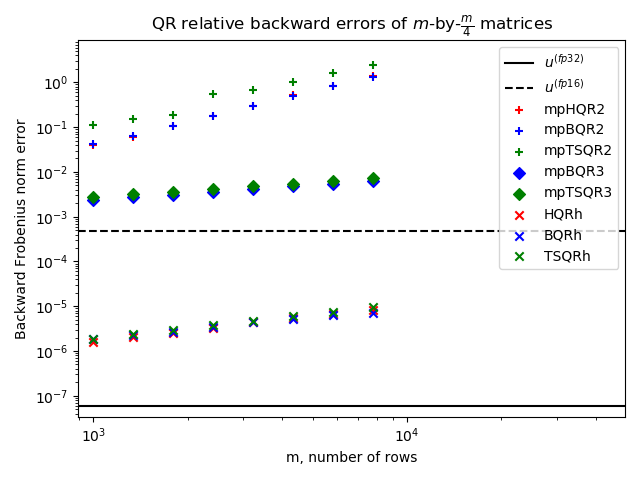
\includegraphics[width=0.45\textwidth]{./figures/sizefig.png}
	%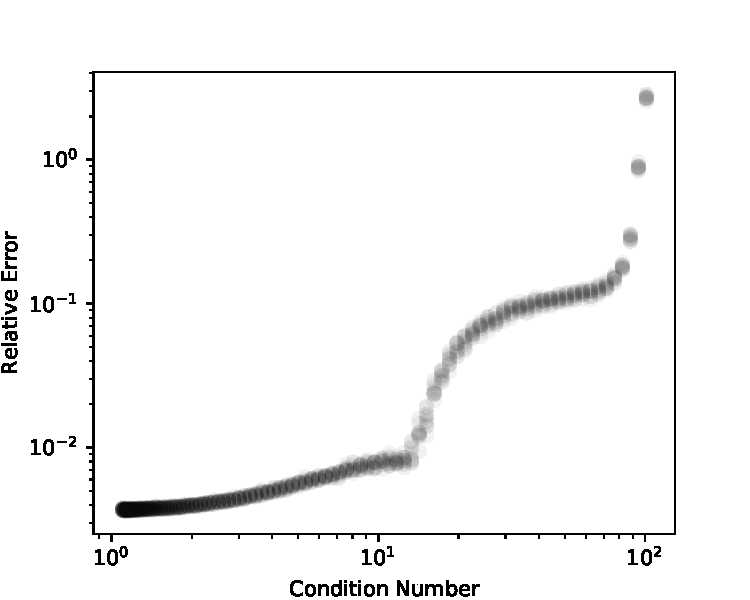
\includegraphics[width=0.45\textwidth]{./figures/unblocked.pdf}
	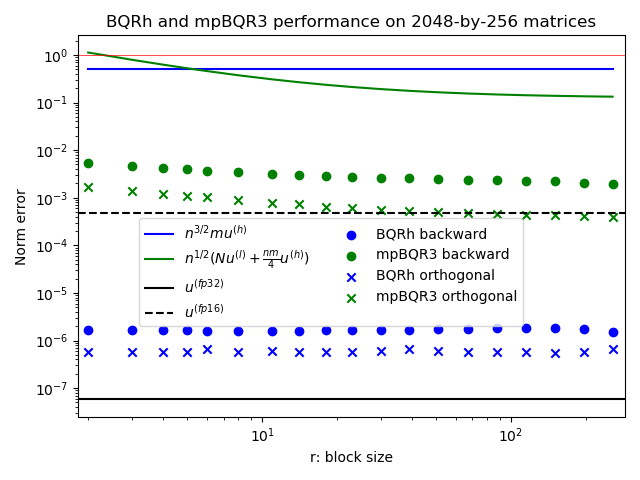
\includegraphics[width=0.45\textwidth]{./figures/mpBQR3-blocksize-1108.png}
	\caption{\label{fig:sizemp3}Left plot: Backward errors of HH QR factorization algorithms in \cref{sec:algo,sec:mpanalysis} with varying matrix sizes. 
		%Right plot: {\tt mpHQR2} errors for $4000$-by-$100$ matrices with varying condition numbers.}
		Right plot: Norm errors of fp32 BQR and {\tt mpBQR3} for $2048$-by-$256$ matrices for varying block sizes.}
	\vspace{-10pt}
\end{figure} 

Next, we varied the block sizes for performing fp32 BQR and {\tt mpBQR3} on $2048$-by-$256$ sized matrices, which were chosen to yield error bounds below 1 for both algorithms.
The right plot of \cref{fig:sizemp3} shows the error bounds and the computed value for the backward error for the two algorithms where the block size $r$ varies from $2$ to $256$. 
The test matrices were generated following example from \cite{Blanchard2019} by setting $\bb{A}={\tt castdown}(\bb{Q}_1\bb{D}\bb{Q}_2)$ where $\bb{Q}_1\in\F_h^{m\times n}$, $\bb{Q}_2\in\F_h^{n\times n}$ are orthogonal and $\bb{D}=\mathrm{Diagonal}(\{\log_{10}(0),\cdots, \log_{10}(-3)\})\in\F_h^{n\times n}$.  
The high precision implementation yields backward error close to $u^{(fp32)}$ and {\tt mpBQR3} yields errors near $u^{(fp16)}$ that follows the downward trend suggested by \cref{eqn:mpBQR3}.
As block sizes increase, {\tt mpBQR3} grows more accurate. 
This trend correlates to $1/N$, the approximate fraction of FLOPs in {\tt mpBQR3} performed in high precision, marked in orange.
%TODO: line Q.
However, the rightmost data for {\tt mpBQR3} (corresponds to $r=n$), is still between 3 and 4 orders of magnitude less accurate than its high precision variant. 
Further studies that directly test speed-ups from bFMAs against the accuracy of {\tt mpBQR3} are needed to fully understand the potential uses for mixed precision QR algorithms.
%There exist applications that are robust to QR factorization errors and could benefit from speed-ups of using bFMAs.

Lastly, we compared {\tt mpTSQR2} against {\tt mpHQR2}.
Note that an empirical comparison of the two algorithms implemented in fp64 arithmetic were reported in \cite{Mori2012}, and we omit the comparison against {\tt mpBQR2} since it performs very similarly to {\tt mpHQR2}.
Following example from \cite{Mori2012}, we used $m$-by-$n$ random matrices, $\bb{A}_{\alpha} = \bb{Q'}(\alpha \bb{E} + \bb{I})/\|\bb{Q'}(\alpha \bb{E} + \bb{I})\|_F$, where $\bb{Q'}\in\mathbb{R}^{m\times n}$ is orthogonal and $\bb{E}\in\R^{n\times n}$ is the matrix of $1$'s. 
We constructed $\bb{Q'}$ by computing the default QR factorization of matrix $\bb{\Omega}\in\F_{fp64}^{4000\times100}$ in Julia, which performs BQR with $r=36$ entirely in fp64 arithmetic, and elements of the random matrix $\bb{\Omega}$ were sampled from the uniform distribution over $[0,1]$.
By construction, $\bb{A}_{\alpha}$ has 2-norm condition number $n\alpha+1$. 
By varying $\alpha$ from {\tt 1e-4} to {\tt 1}, we varied the condition number from $1.1$ to $101$, and we generated $10$ samples for each value of $\alpha$.
The relative backward error, $\|\hat{\bb{Q}}\hat{\bb{R}}-\bb{A}\|_F/\|\bb{A}\|_F$, was computed by casting up $\hat{\bb{Q}}$, $\hat{\bb{R}}$, and $\bb{A}$ to fp64 to compute the Frobenius norms.
Plugging in $m=4000$, $n=100$, $u^{(l)}=u^{(fp16)}$, $u^{(h)}=u^{(fp32)}$, and $c=1$ (for $\tilde{\gamma}$) into the error bounds for {\tt mpHQR2} combined with \cref{eqn:QRA,eqn:QQI} are approximately {\tt 1.179} and {\tt 1.146}.
These error bounds are \emph{relative} and these worst-case bounds do not guarantee errors below 100\%.
The TSQR bounds for the same parameters for $L=1:5$ are even larger, which indicates that stability is not guaranteed. 
The leftmost plot of \cref{fig:allTSQR} shows the backward errors of {\tt mpHQR2} increasing as the theoretical condition numbers of the generated random matrices increase, and these errors correspond to the error data on the vertical axis, $L=0$, of the middle plot.
In addition to the errors from {\tt mpHQR2}, Figure~\ref{fig:allTSQR} shows the errors from {\tt mpTSQR2s} of levels varying from $L=1$ to $L=5$, where each line represents the errors of HQR and variants of TSQR calculated from the same random test matrix.
Figure~\ref{fig:allTSQR} reveals two different trends for the errors as we deepen the complexity of the QR algorithm from {\tt mpHQR2} to {\tt mpTSQR2} with $L=5$. 
One trend occurs for matrices with smaller condition numbers, where {\tt mpHQR2} is stable, but {\tt mpTSQR2} with higher levels yield larger errors. 
Another trend occurs for matrices with higher condition numbers, where single-level and 2-level {\tt mpTSQR2} yield smaller errors than {\tt mpHQR2}. 
In these cases, errors from {\tt mpTSQR2} with 3 or more levels are similar to or worse than their 2-level variants, but generally do not exceed those of {\tt mpHQR2} most of the times.
These results suggests that TSQR can outperform HQR even in mixed precision settings, and particularly when HQR is unstable due to larger condition numbers.
%Although this experiment focused on condition numbers, identifying other properties that point to better performance of TSQR than HQR can further broaden the potential use of mixed precision TSQR in applications.
\begin{figure}[h!]%{r}{.53\textwidth}
	\centering
	%\vspace{-10pt}
	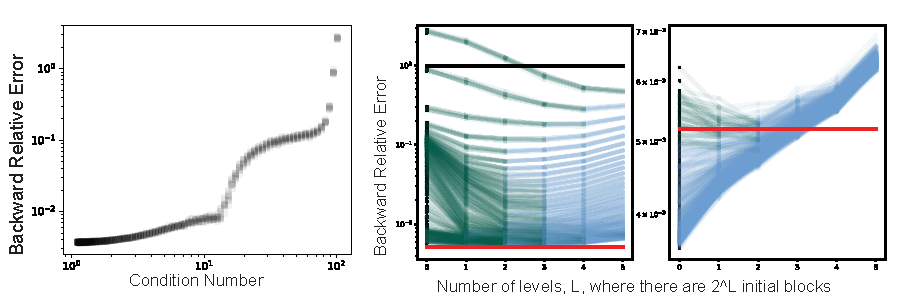
\includegraphics[width=\textwidth]{./figures/allTSQR3.pdf}
	%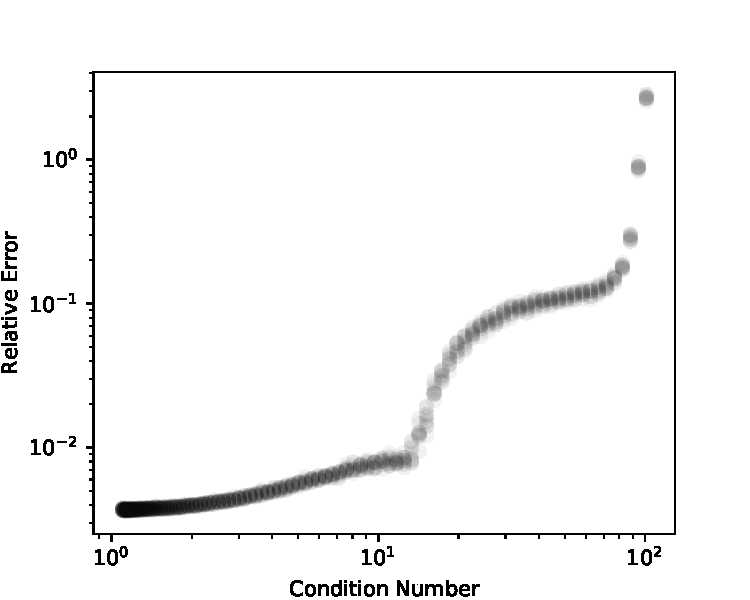
\includegraphics[width=0.35\textwidth]{./figures/unblocked.pdf}
	%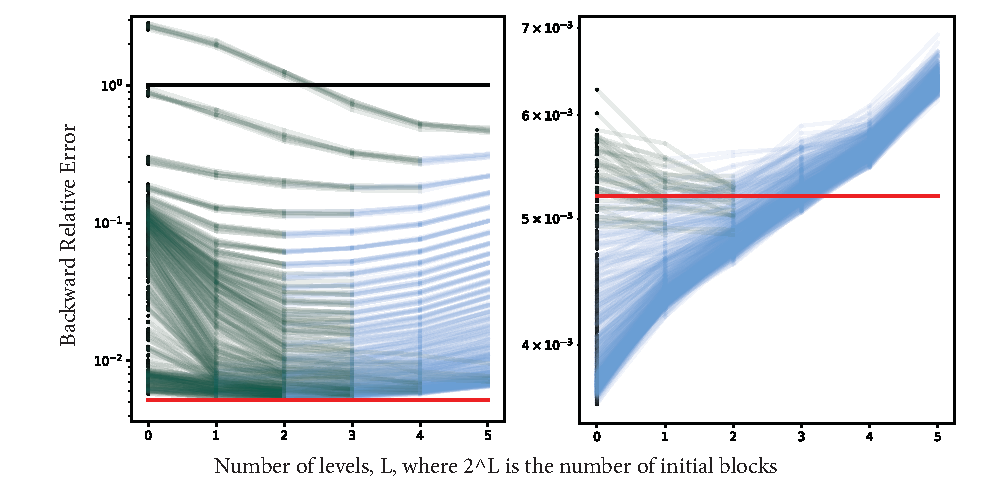
\includegraphics[width=0.64\textwidth]{./figures/allTSQR2.pdf}
	\vspace{-15pt}
	\caption{\label{fig:allTSQR} All plots show the backward relative error for 4000-by-100 sized test matrices. Left: {\tt mpHQR2} on condition numbers ranging from 1.1 to 101;  Middle: {\tt mpTSQR2} on condition numbers ranging from 5.3 to 101; Right:  {\tt mpTSQR2} on condition numbers ranging from 1.1 to 5.3. }
	\vspace{-15pt}
\end{figure}

In conclusion, most of the experiments display the trends that error bounds in \cref{sec:algo,sec:mpanalysis} suggest, and bFMA variants perform in between the high precision and \cref{assump:mp} variants as expected.
Also, a special case is shown that demonstrate {\tt mpTSQR2} can outperform {\tt mpHQR2} despite having higher error bounds.
All of the experiments showed that the actual errors were many orders of magnitude lower than the error bounds even when ill-conditioned, but this discrepancy varied for different mixed precision settings.
For example, backward and forward errors of {\tt mpBQR3} were \emph{only} 2-3 orders of magnitude below the error bounds, whereas the fp32 implementation of BQR yielded errors up to 6 orders of magnitude below the error bounds.
Although further studies with larger problem sizes and timings would be beneficial in developing an {\tt mpBQR3} with the optimal block size, $r$, our experiments confirm the intuition built from the error analysis in \cref{sec:mpanalysis}.
We conducted several numerical experiments to confirm the validity of the error bounds formed in \cref{sec:mpanalysis} by varying size for all algorithms, block sizes in {\tt mpBQR3}, and comparing {\tt mpHQR2} against {\tt mpTSQR2} with varying condition numbers.
We used Julia, a programming language which allows fp16 storage and {\tt castup} and {\tt castdown} operations between types in {fp16, fp32, fp64}, but no built-in fp16 arithmetic.
Therefore, we relied on using \cref{algo:simulate} for $f\in \text{OP} \cup\{{\tt dot\_product}\}$ to simulate \cref{assump:mp} and TensorCore bFMAs.\par

In \cref{sec:algo,sec:mpanalysis}, we gave the forward error bounds for $\bb{R}$ and $\bb{Q}$ separately. 
Since our numerical experiments instead measure a backward error, $\|\hat{\bb{Q}}\hat{\bb{R}}-\bb{A}\|_F$, and an orthogonal error, $\|\hat{\bb{Q}}^{\top}\hat{\bb{Q}}-\bb{I}\|_2$, we show how to convert general forward errors into those computed quantities.
Given $\|(\hat{\bb{R}}-\bb{R})[:,j]\|_2\leq \epsilon_R \|\bb{A}[:,j]\|_2$ and $\|\hat{\bb{Q}}-\bb{Q}\|_F\leq \epsilon_Q$,
\begin{align}
	\|(\hat{\bb{Q}}\hat{\bb{R}}-\bb{A})[:,j]\|_2 &\leq (\epsilon_R+\epsilon_Q + \epsilon_R\epsilon_Q)\|\bb{A}[:,j]\|_2,\;\; j=1:n,\quad \text{see \cite{Higham2002}},\\
	\|\hat{\bb{Q}}\hat{\bb{R}}-\bb{A}\|_F &\leq n^{1/2}(\epsilon_R+\epsilon_Q + \epsilon_R\epsilon_Q)\|\bb{A}\|_F, \label{eqn:QRA} \\
	\|\hat{\bb{Q}}^{\top}\hat{\bb{Q}}-\bb{I}\|_2 &\leq \|\hat{\bb{Q}}^{\top}\hat{\bb{Q}}-\bb{I}\|_F \simeq 2\epsilon_Q,\quad\text{see \cite{Mori2012}} \label{eqn:QQI}.
\end{align}
First, we tested \cref{algo:hhQR,algo:blockHQR,algo:par_tsqr,algo:mpBQR}, {\tt mpHQR2}, {\tt mpBQR2}, and {\tt mpTSQR2} for varying matrix sizes.
We increased the number of rows $m$ from $1000$ to $13949$, while keeping $n=m/4$, $r=n/4$, and $L=2$ and the test matrices were sampled from the standard normal distribution. 
On the left plot of \cref{fig:sizemp3}, we see three clusters which each correspond to: top, \cref{assump:mp}; middle, TensorCore bFMAs; and bottom, uniform precision implementations in fp32.
The high precision and bFMA implementations scale similarly to each other when increasing the matrix size, whereas the \cref{assump:mp} variants grow unstable more quickly.
In addition, while HQR, BQR, and TSQR perform similarly in high precision and when using bFMAs, {\tt mpTSQR2} is less accurate by a quarter to a half order of magnitude in comparison to {\tt mpBQR2} and {\tt mpHQR2}.
The specifications for $m,n,L,M_{l,h}$ for this experiment derive the upper bound for $\|\Delta \bb{Q}_{mpTSQR2}\|_F$, \cref{eqn:mptsqr2Q}, to be larger than that of $\|\Delta \bb{Q}_{mpHQR2}\|_F$, \cref{eqn:mpHQR2Q}.
However, a more careful comparison of {\tt mpHQR2} and {\tt mpTSQR2} show that there exists a regime where {\tt mpTSQR2} can outperform {\tt mpHQR2}.
\begin{figure}[h!]
	\centering
	\vspace{-10pt}
	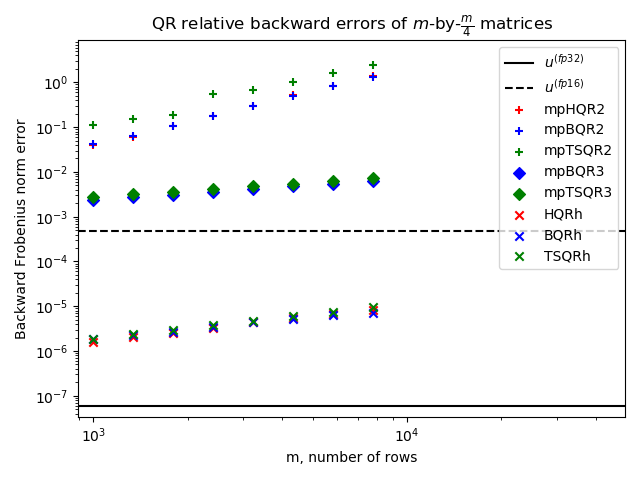
\includegraphics[width=0.45\textwidth]{./figures/sizefig.png}
	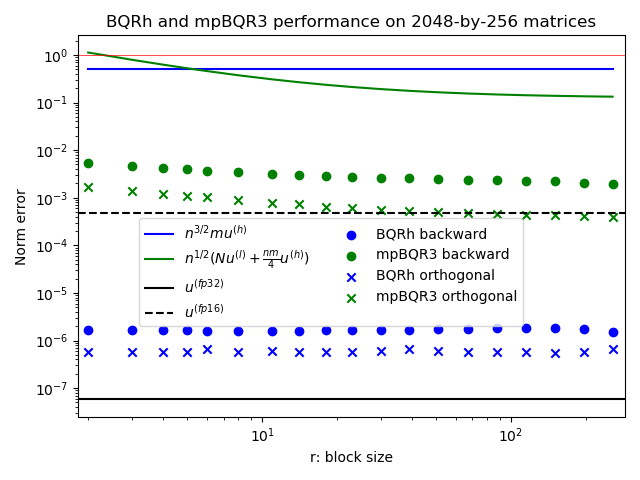
\includegraphics[width=0.45\textwidth]{./figures/mpBQR3-blocksize-1108.png}
	\caption{\label{fig:sizemp3}Left plot: Backward errors of HH QR factorization algorithms in \cref{sec:algo,sec:mpanalysis} with varying matrix sizes.
		Right plot: Norm errors of fp32 BQR and {\tt mpBQR3} for $2048$-by-$256$ matrices for varying block sizes.}
	\vspace{-10pt}
\end{figure} 

Next, we varied the block sizes for performing fp32 BQR and {\tt mpBQR3} on $2048$-by-$256$ sized matrices, which were chosen to yield error bounds below 1 for both algorithms.
The right plot of \cref{fig:sizemp3} shows the error bounds and the computed value for the backward error for the two algorithms where the block size $r$ varies from $2$ to $256$. 
The test matrices were generated following example from \cite{Blanchard2020} by setting $\bb{A}={\tt castdown}(\bb{Q}_1\bb{D}\bb{Q}_2)$ where $\bb{Q}_1\in\F_h^{m\times n}$, $\bb{Q}_2\in\F_h^{n\times n}$ are orthogonal and $\bb{D}=\mathrm{Diagonal}(\{\log_{10}(0),\cdots, \log_{10}(-3)\})\in\F_h^{n\times n}$.  
The high precision implementation yields backward error close to $u^{(fp32)}$ and {\tt mpBQR3} yields errors near $u^{(fp16)}$ that follows the downward trend suggested by \cref{eqn:mpBQR3}.
As block sizes increase, {\tt mpBQR3} grows more accurate. 
This trend correlates to $1/N$, the approximate fraction of FLOPs in {\tt mpBQR3} performed in high precision, marked in orange.
However, the rightmost data for {\tt mpBQR3} (corresponds to $r=n$), is still between 3 and 4 orders of magnitude less accurate than its high precision variant. 
Further studies that directly test speed-ups from bFMAs against the accuracy of {\tt mpBQR3} are needed to fully understand the potential uses for mixed precision QR algorithms.

Lastly, we compared a mixed precision variant of a communication-avoiding QR algorithm ({\tt mpTSQR2}) against a mixed precision variant of the HH QR algorithm ({\tt mpHQR2}).
Note that an empirical comparison of the two algorithms implemented in fp64 arithmetic were reported in \cite{Mori2012}, and we omit the comparison against {\tt mpBQR2} since it performs very similarly to {\tt mpHQR2}.
Following example from \cite{Mori2012}, we used $m$-by-$n$ random matrices, $\bb{A}_{\alpha} = \bb{Q'}(\alpha \bb{E} + \bb{I})/\|\bb{Q'}(\alpha \bb{E} + \bb{I})\|_F$, where $\bb{Q'}\in\mathbb{R}^{m\times n}$ is orthogonal and $\bb{E}\in\R^{n\times n}$ is the matrix of $1$'s. 
We constructed $\bb{Q'}$ by computing the default QR factorization of matrix $\bb{\Omega}\in\F_{fp64}^{4000\times100}$ in Julia, which performs BQR with $r=36$ entirely in fp64 arithmetic, and elements of the random matrix $\bb{\Omega}$ were sampled from the uniform distribution over $[0,1]$.
By construction, $\bb{A}_{\alpha}$ has 2-norm condition number $n\alpha+1$. 
By varying $\alpha$ from {\tt 1e-4} to {\tt 1}, we varied the condition number from $1.1$ to $101$, and we generated $10$ samples for each value of $\alpha$.
The relative backward error, $\|\hat{\bb{Q}}\hat{\bb{R}}-\bb{A}\|_F/\|\bb{A}\|_F$, was computed by casting up $\hat{\bb{Q}}$, $\hat{\bb{R}}$, and $\bb{A}$ to fp64 to compute the Frobenius norms.
Plugging in $m=4000$, $n=100$, $u^{(l)}=u^{(fp16)}$, $u^{(h)}=u^{(fp32)}$, and $c=1$ (for $\tilde{\gamma}$) into the error bounds for {\tt mpHQR2} combined with \cref{eqn:QRA,eqn:QQI} are approximately {\tt 1.179} and {\tt 1.146}.
These error bounds are \emph{relative} and these worst-case bounds do not guarantee errors below 100\%.
The TSQR bounds for the same parameters for $L=1:5$ are even larger, which indicates that stability is not guaranteed. 
The leftmost plot of \cref{fig:allTSQR} shows the backward errors of {\tt mpHQR2} increasing as the theoretical condition numbers of the generated random matrices increase, and these errors correspond to the error data on the vertical axis, $L=0$, of the middle plot.
In addition to the errors from {\tt mpHQR2}, Figure~\ref{fig:allTSQR} shows the errors from {\tt mpTSQR2s} of levels varying from $L=1$ to $L=5$, where each line represents the errors of HQR and variants of TSQR calculated from the same random test matrix.
Figure~\ref{fig:allTSQR} reveals two different trends for the errors as we deepen the complexity of the QR algorithm from {\tt mpHQR2} to {\tt mpTSQR2} with $L=5$. 
One trend occurs for matrices with smaller condition numbers, where {\tt mpHQR2} is stable, but {\tt mpTSQR2} with higher levels yield larger errors. 
Another trend occurs for matrices with higher condition numbers, where single-level and 2-level {\tt mpTSQR2} yield smaller errors than {\tt mpHQR2}. 
In these cases, errors from {\tt mpTSQR2} with 3 or more levels are similar to or worse than their 2-level variants, but generally do not exceed those of {\tt mpHQR2} most of the times.
These results suggests that TSQR can outperform HQR even in mixed precision settings, and particularly when HQR is unstable due to larger condition numbers.
\begin{figure}[h!]%{r}{.53\textwidth}
	\centering
	%\vspace{-10pt}
	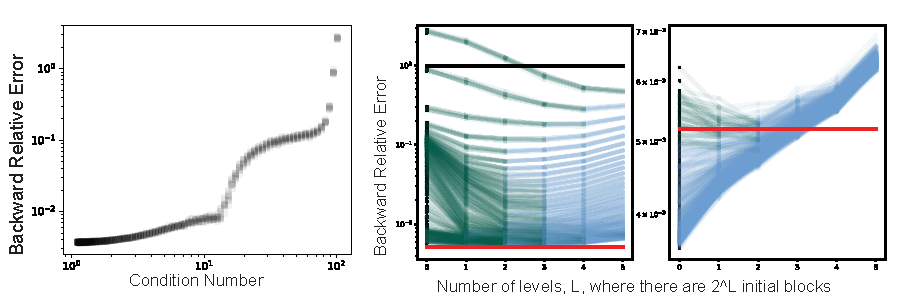
\includegraphics[width=\textwidth]{./figures/allTSQR3.pdf}
	\vspace{-15pt}
	\caption{\label{fig:allTSQR} All plots show the backward relative error for 4000-by-100 sized test matrices. Left: {\tt mpHQR2} on condition numbers ranging from 1.1 to 101;  Middle: {\tt mpTSQR2} on condition numbers ranging from 5.3 to 101; Right:  {\tt mpTSQR2} on condition numbers ranging from 1.1 to 5.3. }
	\vspace{-15pt}
\end{figure}

In conclusion, most of the experiments display the trends that error bounds in \cref{sec:algo,sec:mpanalysis} suggest, and bFMA variants perform in between the high precision and \cref{assump:mp} variants as expected.
Also, a special case is shown that demonstrate {\tt mpTSQR2} can outperform {\tt mpHQR2} despite having higher error bounds.
All of the experiments showed that the actual errors were many orders of magnitude lower than the error bounds even when ill-conditioned, but this discrepancy varied for different mixed precision settings.
For example, backward and forward errors of {\tt mpBQR3} were \emph{only} 2-3 orders of magnitude below the error bounds, whereas the fp32 implementation of BQR yielded errors up to 6 orders of magnitude below the error bounds.
Although further studies with larger problem sizes and timings would be beneficial in developing an {\tt mpBQR3} with the optimal block size, $r$, our experiments confirm the intuition built from the error analysis in \cref{sec:mpanalysis}.
\section{Conclusion}
The development of GPUs that optimize low precision floating point arithmetic have accelerated the interest in half and mixed precision algorithms that naturally reduces the bandwidth and storage needs. 
Loss in precision, stability, and representable range offset for those advantages, but these shortcomings may have little to no impact in some applications.
It may even be possible to navigate around those drawbacks with algorithmic design. \par
We present the algorithm and standard error analysis of HQR and its blocked variants (BQR and TSQR), modify the algorithms to support two mixed precision settings, and performed error analysis that accurately bound the mixed precision versions.
One mixed precision setting is that of NVIDIA's TensorCore bFMAs, and the other is an ad hoc setting that mimics the bFMAs at the level of inner products.
These two are presented to offer mixed precision arithmetic at both level-2 and 3 BLAS operations and can be applied to other linear algebra tools as well.
The new error bounds more accurately describe how rounding errors are accumulated in mixed precision settings.
For a given problem, available hardware, and some error tolerance, these bounds can be used to first narrow down which QR factorization algorithms are feasible. 
Then, the speed-ups from the hardware specifications can be considered next to choose the most appropriate settings within the algorithms (i.e. block size $r$ in BQR or number of levels, $L$, in TSQR).
We found that TSQR can outperform HQR under \cref{assump:mp} for ill-conditioned, extremely overdetermined cases even when the error bounds imply the opposite.
While an optimistic interpretation of this result would be that algorithms like TSQR are more robust against lower precision arithmetic, further research is needed to explore other divide-and-conquer methods that can harness parallel capabilities.
Meanwhile, we should rely on the error bounds formed in \cref{sec:mpanalysis}.
\bibliographystyle{siamplain}%ieeetr
\bibliography{../../../../../library.bib,../../../../../sans_library.bib,./report.bib}

\end{document}
